\cotefile{148}

\scanpage{21}

\figure{\begin{tikzpicture}[x=0.009cm,y=-0.009cm,line cap=round,line join=round]
% The short isolated strokes and the six long strokes around the sketches.
\draw[line width=.65pt] (222,143)..controls(245,131)and(261,132)..(289,149);
\begin{scope}[shift={(376,449)}]
\draw[gray!65,line width=.35pt] (9,48) -- (14,46);
\draw[line width=.6pt] (15,45) .. controls (18,42) and (18,40) .. (20,38);
\draw[line width=.8pt] (21,36) .. controls (22,34) and (23,32) .. (25,30);
\draw[gray!75,line width=.45pt] (27,29) -- (31,24) -- (35,21);
\draw[gray!65,line width=.4pt] (38,19) -- (39,16);
\draw[gray!65,line width=.35pt] (40,15) -- (46,12);
\draw[gray!65,line width=.35pt] (48,10) -- (53,7);
\end{scope}
\draw[gray!65,line width=.4pt] (800,94)..controls(789,88)and(788,179)..(792,260)..controls(790,319)and(789,367)..(799,382)..controls(808,373)and(808,362)..(805,337)..controls(802,251)and(810,137)..(800,94);
\draw[gray!65,line width=.4pt] (395,230)..controls(475,303)and(552,387)..(653,501);
\draw[gray!65,line width=.4pt] (1047,387)..controls(1106,337)and(1169,259)..(1192,242)--(1210,231);
\draw[gray!65,line width=.4pt] (348,773)..controls(431,717)and(525,651)..(597,595);
\draw[gray!65,line width=.4pt] (759,688)..controls(764,781)and(750,905)..(756,1000);
\draw[gray!65,line width=.4pt] (866,624)..controls(940,675)and(1011,757)..(1086,805);

% The larger sketch, with visible partial retracings and six separated transverse strokes.
\begin{scope}[shift={(645,415)}]
\draw[line width=.75pt] (20,159) .. controls (51,116) and (93,58) .. (123,17);
\draw[line width=.45pt] (24,158) .. controls (57,113) and (96,52) .. (124,19);
\draw[line width=.45pt] (22,151) -- (40,126) -- (49,115);
\draw[line width=.45pt] (88,67) -- (101,45) -- (121,17);
\draw[line width=.65pt] (124,19) .. controls (146,46) and (155,70) .. (178,91) .. controls (188,102) and (201,107) .. (208,115);
\draw[line width=.9pt] (211,120) .. controls (196,144) and (172,174) .. (156,196);
\draw[line width=.85pt] (125,24) .. controls (128,54) and (136,91) .. (140,126) .. controls (145,149) and (150,183) .. (156,202);
\draw[line width=.6pt] (26,159) .. controls (66,178) and (116,199) .. (151,207);
\draw[line width=.55pt] (36,152) .. controls (41,148) and (47,148) .. (51,149);
\draw[line width=.5pt] (60,144) .. controls (64,141) and (71,141) .. (77,140);
\draw[line width=.5pt] (88,137) .. controls (92,133) and (97,134) .. (101,134);
\draw[line width=.45pt] (112,132) -- (122,126);
\draw[line width=.4pt] (143,126) .. controls (149,123) and (155,121) .. (162,121);
\draw[line width=.4pt] (173,120) .. controls (180,117) and (190,115) .. (194,117) -- (202,115);
\end{scope}

% Smaller sketch: literal tapered dark patches, without assigned arrow directions.
\begin{scope}[shift={(900,330)}]
\draw[gray!80,line width=.45pt] (21,143) .. controls (32,108) and (70,55) .. (90,21);
\draw[gray!80,line width=.35pt] (23,136) .. controls (43,105) and (70,62) .. (87,28);
\draw[gray!80,line width=.55pt] (94,18) .. controls (107,22) and (109,31) .. (123,39) .. controls (142,53) and (151,56) .. (158,63) -- (176,75);
\draw[gray!80,line width=.6pt] (186,90) .. controls (165,113) and (150,141) .. (135,163);
\draw[gray!80,line width=.35pt] (181,91) .. controls (164,112) and (148,133) .. (135,151);
\draw[gray!80,line width=.45pt] (92,23) .. controls (98,42) and (104,62) .. (112,82) .. controls (122,113) and (130,141) .. (135,167);
\draw[gray!80,line width=.45pt] (117,94) .. controls (124,112) and (130,127) .. (135,143);
\draw[gray!80,line width=.5pt] (24,139) .. controls (49,147) and (92,165) .. (128,170);
\draw[gray!80,line width=.55pt] (18,135) .. controls (48,127) and (74,121) .. (98,114);
\draw[gray!80,line width=.45pt] (131,102) .. controls (149,96) and (163,92) .. (176,87);
\draw[gray!80,line width=.35pt] (16,179) -- (21,178) .. controls (51,152) and (79,126) .. (101,109);
\draw[gray!80,line width=.35pt] (102,109) .. controls (121,88) and (138,70) .. (148,56);
\draw[line width=.55pt] (68,151) .. controls (79,138) and (89,126) .. (98,117);
\fill (66,154) -- (70,143) -- (80,136) -- (76,145) -- cycle;
\draw[line width=.65pt] (91,123) -- (98,120);
\draw[line width=.55pt] (111,110) -- (116,103);
\draw[line width=.75pt] (122,98) -- (126,91);
\draw[line width=.7pt] (132,86) .. controls (139,76) and (144,69) .. (149,59);
\fill (149,56) -- (147,67) -- (141,72) -- (143,63) -- cycle;
\draw[line width=.75pt] (101,111) -- (110,101) -- (115,91) -- (128,77);
\fill (113,93) -- (119,82) -- (132,74) -- (125,84) -- cycle;
\draw[line width=.6pt] (97,108) -- (105,97);
\draw[line width=.6pt] (116,77) -- (125,72);
\draw[line width=.6pt] (134,69) -- (140,65);
\end{scope}
\end{tikzpicture}}

\margin{20}

\scanpage{22}

\texttt{//* GUTS 0055 I}

\figure{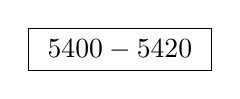
\begin{tikzpicture}
\node[draw,inner xsep=7pt,inner ysep=4pt] {$5400-5420$};
\end{tikzpicture}}

\margin{\handwritten{(93) 51, 91, 00 \quad 411.}}

\figure{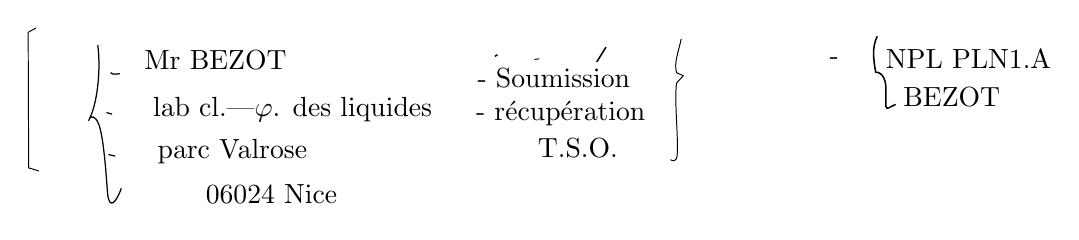
\begin{tikzpicture}[x=0.0065cm,y=-0.0065cm,
  every node/.style={anchor=west,inner sep=0pt,font=\normalsize}]
% The outer brackets finish above the postcode; the inner brace continues down to it.
\draw[line width=0.35pt] (38,9) -- (23,17) -- (24,282) -- (44,288);
\draw[line width=0.35pt] (1299,30) .. controls (1294,54) and (1284,78) .. (1290,96)
  -- (1303,102) -- (1290,116) .. controls (1285,151) and (1294,222) .. (1291,259)
  .. controls (1289,270) and (1283,269) .. (1278,266);
\draw[line width=0.45pt] (159,42) .. controls (165,87) and (159,147) .. (146,179)
  -- (141,190) .. controls (145,177) and (155,181) .. (161,197)
  .. controls (171,223) and (176,304) .. (178,330)
  .. controls (181,366) and (195,350) .. (205,322);
% Three short strokes at the left of the address lines, kept as drawn marks.
\draw[line width=0.45pt] (184,96) .. controls (190,101) and (196,98) .. (202,98);
\draw[line width=0.45pt] (176,174) -- (187,177);
\draw[line width=0.45pt] (180,256) -- (193,259);
\node at (249,72) {\handwritten{Mr BEZOT}};
\node at (266,168) {\handwritten{lab \unsure{cl.|\(\varphi\).} des liquides}};
\node at (275,251) {\handwritten{parc Valrose}};
\node at (369,333) {\handwritten{06024 Nice}};
% Detached dark strokelets above the annotation; no word is inferred.
\draw[line width=.55pt] (935,64)--(940,61);
\draw[line width=.35pt] (1012,70)--(1022,69);
\draw[line width=.55pt] (1134,75)--(1152,46);
\node at (900,107) {\handwritten{- Soumission}};
\node at (897,176) {\handwritten{- récupération}};
\node at (1018,244) {\handwritten{T.S.O.}};
\node at (1588,69) {\handwritten{-}};
\draw[line width=0.55pt] (1682,25) .. controls (1671,47) and (1675,72) .. (1679,95)
  .. controls (1693,95) and (1700,111) .. (1699,133)
  -- (1699,162) .. controls (1700,170) and (1708,162) .. (1718,158);
\node at (1698,69) {\handwritten{NPL PLN1.A}};
\node at (1732,143) {\handwritten{BEZOT}};
\end{tikzpicture}}

\figure{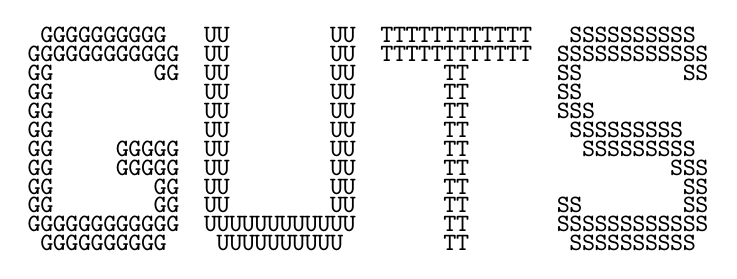
\begin{tikzpicture}[x=0.16cm,y=-0.24cm,
 every node/.style={inner sep=0pt,font=\ttfamily\small}]
\foreach \x/\y in {1/0,2/0,3/0,4/0,5/0,6/0,7/0,8/0,9/0,10/0,0/1,1/1,2/1,3/1,4/1,5/1,6/1,7/1,8/1,9/1,10/1,11/1,0/2,1/2,10/2,11/2,0/3,1/3,0/4,1/4,0/5,1/5,0/6,1/6,7/6,8/6,9/6,10/6,11/6,0/7,1/7,7/7,8/7,9/7,10/7,11/7,0/8,1/8,10/8,11/8,0/9,1/9,10/9,11/9,0/10,1/10,2/10,3/10,4/10,5/10,6/10,7/10,8/10,9/10,10/10,11/10,1/11,2/11,3/11,4/11,5/11,6/11,7/11,8/11,9/11,10/11}
  {\node at (\x,\y) {G};}
\foreach \x/\y in {14/0,15/0,24/0,25/0,14/1,15/1,24/1,25/1,14/2,15/2,24/2,25/2,14/3,15/3,24/3,25/3,14/4,15/4,24/4,25/4,14/5,15/5,24/5,25/5,14/6,15/6,24/6,25/6,14/7,15/7,24/7,25/7,14/8,15/8,24/8,25/8,14/9,15/9,24/9,25/9,14/10,15/10,16/10,17/10,18/10,19/10,20/10,21/10,22/10,23/10,24/10,25/10,15/11,16/11,17/11,18/11,19/11,20/11,21/11,22/11,23/11,24/11}
  {\node at (\x,\y) {U};}
\foreach \x/\y in {28/0,29/0,30/0,31/0,32/0,33/0,34/0,35/0,36/0,37/0,38/0,39/0,28/1,29/1,30/1,31/1,32/1,33/1,34/1,35/1,36/1,37/1,38/1,39/1,33/2,34/2,33/3,34/3,33/4,34/4,33/5,34/5,33/6,34/6,33/7,34/7,33/8,34/8,33/9,34/9,33/10,34/10,33/11,34/11}
  {\node at (\x,\y) {T};}
\foreach \x/\y in {43/0,44/0,45/0,46/0,47/0,48/0,49/0,50/0,51/0,52/0,42/1,43/1,44/1,45/1,46/1,47/1,48/1,49/1,50/1,51/1,52/1,53/1,42/2,43/2,52/2,53/2,42/3,43/3,42/4,43/4,44/4,43/5,44/5,45/5,46/5,47/5,48/5,49/5,50/5,51/5,44/6,45/6,46/6,47/6,48/6,49/6,50/6,51/6,52/6,51/7,52/7,53/7,52/8,53/8,42/9,43/9,52/9,53/9,42/10,43/10,44/10,45/10,46/10,47/10,48/10,49/10,50/10,51/10,52/10,53/10,43/11,44/11,45/11,46/11,47/11,48/11,49/11,50/11,51/11,52/11}
  {\node at (\x,\y) {S};}
\end{tikzpicture}}

\begin{tabular}{l}
\texttt{****P END STC 55 GUTS}\quad\texttt{ROOM}\quad\texttt{10.32.40 AM 09 JUN 82 R6.PR1}\quad\texttt{SYS JES2 STC 55 END P****}\\
\texttt{****P END STC 55 GUTS}\quad\texttt{ROOM}\quad\texttt{10.32.40 AM 09 JUN 82 R6.PR1}\quad\texttt{SYS JES2 STC 55 END P****}\\
\texttt{****P END STC 55 GUTS}\quad\texttt{ROOM}\quad\texttt{10.32.40 AM 09 JUN 82 R6.PR1}\quad\texttt{SYS JES2 STC 55 END P****}\\
\texttt{****P END STC 55 GUTS}\quad\texttt{ROOM}\quad\texttt{10.32.40 AM 09 JUN 82 R6.PR1}\quad\texttt{SYS JES2 STC 55 END P****}\\
\texttt{****P END STC 55 GUTS}\quad\texttt{ROOM}\quad\texttt{10.32.40 AM 09 JUN 82 R6.PR1}\quad\texttt{SYS JES2 STC 55 END P****}\\
\texttt{****P END STC 55 GUTS}\quad\texttt{ROOM}\quad\texttt{10.32.40 AM 09 JUN 82 R6.PR1}\quad\texttt{SYS JES2 STC 55 END P****}
\end{tabular}

\margin{21}

\scanpage{23}

\begin{flushright}
\texttt{AVANCE SUR PROGRAMMATION AU 26/0}
\end{flushright}

\texttt{MAIN-D}\inserted{'}\texttt{OEUVRE NECESSAIRES A LA FABRICATION DE 1 S}

\begin{tabular}{lll}
002&TRONCONNAGE ALU&0,18 HEURES\\
004&POINCONNAGE ALU&0,18 HEURES\\
013&SOUDURE SKYDOME&0,34 HEURES\\
020&EBARBAGE&0,20 HEURES\\
021&PLAQUES&0,16 HEURES\\
025&COLLAGE&0,42 \unsure{HEURES}\\
026&MONTAGE SKYDOME&1,08 \unsure{HEURES}
\end{tabular}

\texttt{CHARGE GLOBALE MAIN-D OEUVRE POUR \unsure{LA FABRICATION} DE}

\texttt{COUT PRODUCTION \quad 418,60 FRS \quad \unsure{PRIX DE CES}}

\figure{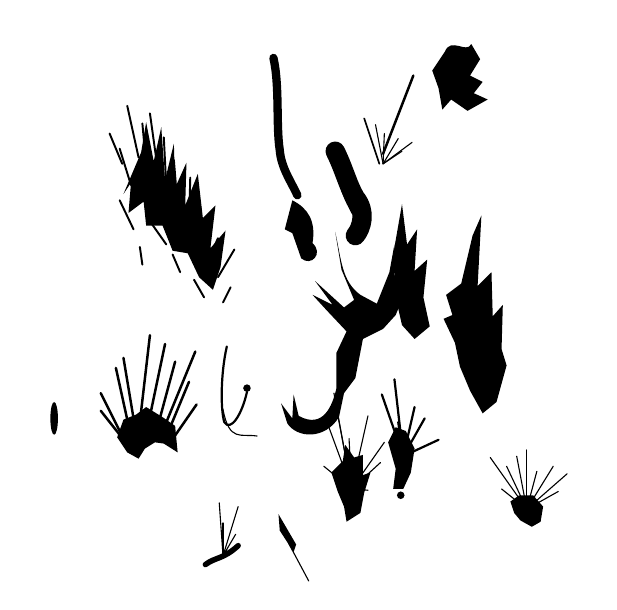
\begin{tikzpicture}[x=0.016cm,y=-0.016cm,line cap=round,line join=round]
\clip (0,0) rectangle (445,440);
\fill (331,19) .. controls (336,7) and (348,21) .. (352,13)
 -- (359,25) -- (351,38) -- (361,43) -- (354,52)
 -- (365,57) -- (349,66) -- (336,57) -- (329,65)
 -- (326,48) -- (321,34) -- cycle;
\draw[line width=3pt] (195,24) .. controls (200,46) and (197,78) .. (200,97)
 .. controls (201,111) and (209,122) .. (214,133);
\fill (90,99) -- (94,75) -- (100,106) -- (106,79) -- (109,121)
 -- (116,92) -- (117,127) -- (126,107) -- (125,141)
 -- (135,116) -- (139,151) -- (149,141) -- (145,175)
 -- (157,161) -- (153,190) -- (147,208) -- (136,198)
 -- (127,179) -- (115,177) -- (107,157) -- (94,157)
 -- (92,138) -- (80,147) -- (82,123) -- (76,132) -- cycle;
\foreach \a/\b/\c/\d in {75/108/65/84,82/125/73/96,88/103/79/62,95/120/91/76,103/111/97/68,110/126/108/87,119/142/116/105,128/157/129/119,136/177/137/142,143/185/151/167,151/198/164/176,84/160/73/137,110/172/98/155,121/194/115/180,140/214/132/200,91/188/89/174,155/218/161/206}
 {\draw[line width=0.7pt] (\a,\b)--(\c,\d);}
\fill (210,137) .. controls (222,143) and (229,153) .. (226,171)
 .. controls (235,179) and (225,190) .. (217,183)
 -- (210,163) -- (204,160) -- cycle;
\draw[line width=7pt] (244,98) .. controls (251,112) and (254,125) .. (260,135)
 .. controls (269,146) and (265,159) .. (260,165);
\draw[line width=3pt] (249,118) .. controls (252,132) and (257,140) .. (260,146);
\fill (244,162) .. controls (249,184) and (249,201) .. (264,212)
 -- (277,219) -- (287,194) -- (291,172) -- (291,197)
 -- (301,183) -- (299,211) -- (292,228) -- (282,239)
 -- (266,247) -- (260,278) -- (251,290) -- (247,309)
 .. controls (236,327) and (214,326) .. (206,314)
 -- (201,298) -- (210,310) -- (211,291) -- (215,308)
 .. controls (235,319) and (242,299) .. (245,286)
 -- (245,258) -- (253,241) -- (237,224) -- (226,212)
 -- (242,220) -- (228,201) -- (251,222) -- (259,216)
 -- (249,192) -- cycle;
\fill (297,140) -- (301,172) -- (309,160) -- (307,193)
 -- (317,184) -- (314,214) -- (319,237) -- (307,247)
 -- (297,236) -- (292,214) -- (290,180) -- cycle;
\fill (344,203) -- (353,165) -- (360,149) -- (357,205)
 -- (368,194) -- (369,229) -- (377,220) -- (376,255)
 -- (380,268) -- (372,297) -- (361,306) -- (351,288)
 -- (343,269) -- (339,250) -- (330,231) -- (337,228)
 -- (332,212) -- cycle;
\draw[line width=0.9pt] (282,100)--(306,38);
\draw[line width=0.6pt] (279,108)--(267,72);
\foreach \a/\b in {276/77,283/84,294/88,305/91,297/98}
 {\draw (282,108)--(\a,\b);}
\fill (21,310) ellipse (3 and 13);
\fill (79,337) -- (71,325) -- (76,311) -- (86,307) -- (94,301)
 -- (107,309) -- (117,316) -- (119,337) -- (108,330)
 -- (101,329) -- (93,334) -- (88,342) -- cycle;
\foreach \a/\b/\c/\d in {77/328/58/290,81/320/70/270,85/316/76/262,89/313/97/244,96/313/109/251,103/317/117/265,108/318/133/257,111/322/128/281,116/325/134/299,73/323/58/304}
 {\draw[line width=0.9pt] (\a,\b)--(\c,\d);}
\draw[line width=0.8pt] (158,253) .. controls (153,275) and (153,303) .. (156,313)
 .. controls (161,321) and (170,307) .. (174,289);
\fill (174,286) circle (3);
\draw (155,303) .. controls (160,329) and (169,322) .. (182,324);
\fill (246,368) -- (241,353) -- (250,344) -- (252,331) -- (259,341)
 -- (266,339) -- (266,355) -- (272,353) -- (267,369)
 -- (264,385) -- (253,392) -- (251,380) -- cycle;
\foreach \a/\b in {239/317,243/290,246/307,255/326,270/308,283/329,280/345,270/367,235/348}
 {\draw (257,366)--(\a,\b);}
\fill (292,350) -- (286,329) -- (292,317) -- (300,320)
 -- (307,334) -- (304,353) -- (298,366) -- (290,366) -- cycle;
\foreach \a/\b in {281/291,291/279,294/313,307/301,315/310,326/327}
 {\draw[line width=0.8pt] (298,340)--(\a,\b);}
\fill (296,371) circle (3);
\fill (386,385) -- (383,376) -- (390,371) -- (401,371)
 -- (409,380) -- (407,392) -- (400,396) -- (391,391) -- cycle;
\foreach \a/\b in {367/341,380/348,388/340,396/335,404/352,417/348,428/354,421/368,376/366}
 {\draw (396,382)--(\a,\b);}
\draw[line width=2pt] (141,426) .. controls (149,420) and (155,422) .. (167,411);
\foreach \a/\b in {152/377,155/393,167/380,165/402,158/414}
 {\draw (155,419)--(\a,\b);}
\fill (199,386) -- (200,399) -- (211,416) -- (213,410) -- cycle;
\draw (207,409)--(223,439);
\end{tikzpicture}}
% crop-candidate: scan 23

\figure{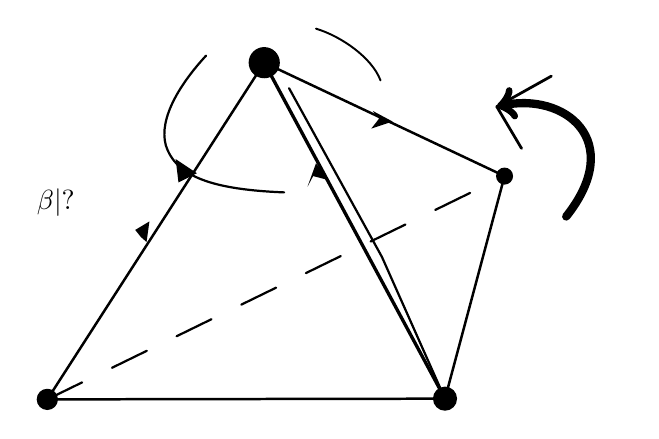
\begin{tikzpicture}[x=0.009cm,y=-0.009cm,line cap=round,line join=round]
\coordinate (A) at (67,550);
\coordinate (B) at (373,75);
\coordinate (C) at (628,549);
\coordinate (D) at (712,235);
\draw[line width=0.9pt] (A)--(B)--(D)--(C)--(A);
\draw[line width=1.2pt] (B)--(C);
\draw[line width=0.8pt] (408,111)--(539,349)--(C);
\draw[dash pattern=on 14pt off 12pt,line width=0.8pt] (A)--(D);
\fill (A) circle (15);
\fill (B) circle (22);
\fill (C) circle (17);
\fill (D) circle (12);
\fill (191,311)--(211,299)--(207,328)--(199,321)--cycle;
\fill (526,143)--(554,158)--(524,168)--(535,154)--cycle;
\fill (446,217)--(465,241)--(442,235)--(434,250)--cycle;
\draw[line width=0.7pt] (446,27) .. controls (482,38) and (525,68) .. (537,100);
\draw[line width=0.8pt] (291,65) .. controls (255,104) and (224,153) .. (234,191)
 .. controls (248,237) and (303,254) .. (401,258);
\fill (248,211)--(278,231)--(252,244)--cycle;
\draw[line width=3pt,->] (799,292) .. controls (884,185) and (797,116) .. (701,137);
\draw[line width=1pt] (701,137)--(778,94);
\draw[line width=1pt] (701,137)--(736,196);
\node at (79,273) {$\unsure{\beta|?}$};
\end{tikzpicture}}

\diagram{\begin{tikzcd}[column sep=small]
\left.\begin{array}{l}\deleted{\deleted{6}\inserted{4}\text{ hexagones}}\\\deleted{4\text{ sommets}}\end{array}\right\}
\arrow[r,bend left]
&
\begin{array}{l}
8\text{ triangles}\\
4\text{ sommets d'ordre }6\\
12\text{ arêtes}
\end{array}
\end{tikzcd}}

\[
\unsure{G|A|a}_{\unsure{4}}
\]

\[
\deleted{\unsure{\widetilde{\mathfrak S}_3}}:
\qquad \mu_6\times(\mathbb Z/2\mathbb Z)^2
\]
\[
\mu_4\times(\mathbb Z/2\mathbb Z)^2
\]

\uline{Hexagone}

\uline{Orienté}

\figure{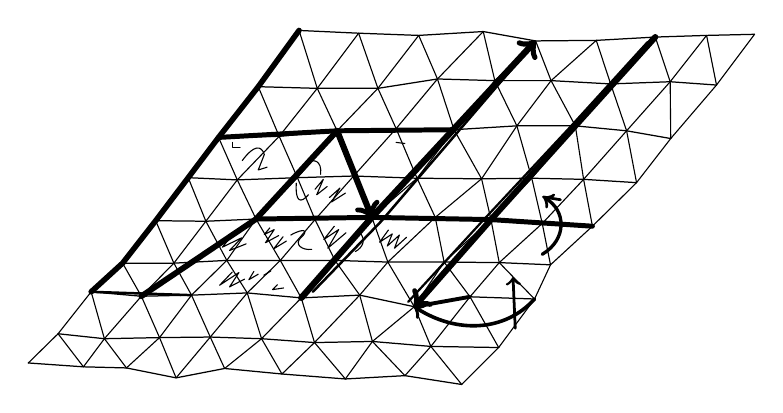
\begin{tikzpicture}[x=0.007cm,y=-0.007cm,line cap=round,line join=round]
\draw[line width=0.45pt] (506,40)--(614,45)--(723,49)--(840,42)--(935,59)--(1045,58)--(1152,52)--(1245,49)--(1332,47);
\draw[line width=0.45pt] (432,142)--(539,145)--(649,145)--(757,128)--(861,131)--(963,131)--(1071,137)--(1179,133)--(1263,139);
\draw[line width=0.45pt] (360,234)--(470,232)--(575,222)--(682,218)--(787,220)--(901,213)--(1007,213)--(1100,222)--(1180,236);
\draw[line width=0.45pt] (305,307)--(394,311)--(503,307)--(605,304)--(720,308)--(837,309)--(928,308)--(1022,310)--(1118,316);
\draw[line width=0.45pt] (246,385)--(337,386)--(428,382)--(535,383)--(638,379)--(753,379)--(854,383)--(947,390)--(1038,395);
\draw[line width=0.45pt] (186,462)--(279,462)--(375,457)--(472,457)--(571,457)--(667,460)--(769,460)--(869,461)--(962,465);
\draw[line width=0.45pt] (129,514)--(220,522)--(311,520)--(412,516)--(510,525)--(616,520)--(715,541)--(816,523)--(933,527);
\draw[line width=0.45pt] (69,590)--(153,599)--(253,597)--(345,596)--(438,599)--(534,606)--(639,604)--(745,613)--(868,615);
\draw[line width=0.45pt] (15,643)--(115,650)--(193,652)--(283,670)--(371,653)--(475,663)--(590,672)--(698,666)--(801,682);
\draw[line width=0.4pt] (506,40)--(432,142);
\draw[line width=0.4pt] (506,40)--(539,145);
\draw[line width=0.4pt] (614,45)--(539,145);
\draw[line width=0.4pt] (614,45)--(649,145);
\draw[line width=0.4pt] (723,49)--(649,145);
\draw[line width=0.4pt] (723,49)--(757,128);
\draw[line width=0.4pt] (840,42)--(757,128);
\draw[line width=0.4pt] (840,42)--(861,131);
\draw[line width=0.4pt] (935,59)--(861,131);
\draw[line width=0.4pt] (935,59)--(963,131);
\draw[line width=0.4pt] (1045,58)--(963,131);
\draw[line width=0.4pt] (1045,58)--(1071,137);
\draw[line width=0.4pt] (1152,52)--(1071,137);
\draw[line width=0.4pt] (1152,52)--(1179,133);
\draw[line width=0.4pt] (1245,49)--(1179,133);
\draw[line width=0.4pt] (1245,49)--(1263,139);
\draw[line width=0.4pt] (1332,47)--(1263,139);
\draw[line width=0.4pt] (432,142)--(360,234);
\draw[line width=0.4pt] (432,142)--(470,232);
\draw[line width=0.4pt] (539,145)--(470,232);
\draw[line width=0.4pt] (539,145)--(575,222);
\draw[line width=0.4pt] (649,145)--(575,222);
\draw[line width=0.4pt] (649,145)--(682,218);
\draw[line width=0.4pt] (757,128)--(682,218);
\draw[line width=0.4pt] (757,128)--(787,220);
\draw[line width=0.4pt] (861,131)--(787,220);
\draw[line width=0.4pt] (861,131)--(901,213);
\draw[line width=0.4pt] (963,131)--(901,213);
\draw[line width=0.4pt] (963,131)--(1007,213);
\draw[line width=0.4pt] (1071,137)--(1007,213);
\draw[line width=0.4pt] (1071,137)--(1100,222);
\draw[line width=0.4pt] (1179,133)--(1100,222);
\draw[line width=0.4pt] (1179,133)--(1180,236);
\draw[line width=0.4pt] (1263,139)--(1180,236);
\draw[line width=0.4pt] (360,234)--(305,307);
\draw[line width=0.4pt] (360,234)--(394,311);
\draw[line width=0.4pt] (470,232)--(394,311);
\draw[line width=0.4pt] (470,232)--(503,307);
\draw[line width=0.4pt] (575,222)--(503,307);
\draw[line width=0.4pt] (575,222)--(605,304);
\draw[line width=0.4pt] (682,218)--(605,304);
\draw[line width=0.4pt] (682,218)--(720,308);
\draw[line width=0.4pt] (787,220)--(720,308);
\draw[line width=0.4pt] (787,220)--(837,309);
\draw[line width=0.4pt] (901,213)--(837,309);
\draw[line width=0.4pt] (901,213)--(928,308);
\draw[line width=0.4pt] (1007,213)--(928,308);
\draw[line width=0.4pt] (1007,213)--(1022,310);
\draw[line width=0.4pt] (1100,222)--(1022,310);
\draw[line width=0.4pt] (1100,222)--(1118,316);
\draw[line width=0.4pt] (1180,236)--(1118,316);
\draw[line width=0.4pt] (305,307)--(246,385);
\draw[line width=0.4pt] (305,307)--(337,386);
\draw[line width=0.4pt] (394,311)--(337,386);
\draw[line width=0.4pt] (394,311)--(428,382);
\draw[line width=0.4pt] (503,307)--(428,382);
\draw[line width=0.4pt] (503,307)--(535,383);
\draw[line width=0.4pt] (605,304)--(535,383);
\draw[line width=0.4pt] (605,304)--(638,379);
\draw[line width=0.4pt] (720,308)--(638,379);
\draw[line width=0.4pt] (720,308)--(753,379);
\draw[line width=0.4pt] (837,309)--(753,379);
\draw[line width=0.4pt] (837,309)--(854,383);
\draw[line width=0.4pt] (928,308)--(854,383);
\draw[line width=0.4pt] (928,308)--(947,390);
\draw[line width=0.4pt] (1022,310)--(947,390);
\draw[line width=0.4pt] (1022,310)--(1038,395);
\draw[line width=0.4pt] (1118,316)--(1038,395);
\draw[line width=0.4pt] (246,385)--(186,462);
\draw[line width=0.4pt] (246,385)--(279,462);
\draw[line width=0.4pt] (337,386)--(279,462);
\draw[line width=0.4pt] (337,386)--(375,457);
\draw[line width=0.4pt] (428,382)--(375,457);
\draw[line width=0.4pt] (428,382)--(472,457);
\draw[line width=0.4pt] (535,383)--(472,457);
\draw[line width=0.4pt] (535,383)--(571,457);
\draw[line width=0.4pt] (638,379)--(571,457);
\draw[line width=0.4pt] (638,379)--(667,460);
\draw[line width=0.4pt] (753,379)--(667,460);
\draw[line width=0.4pt] (753,379)--(769,460);
\draw[line width=0.4pt] (854,383)--(769,460);
\draw[line width=0.4pt] (854,383)--(869,461);
\draw[line width=0.4pt] (947,390)--(869,461);
\draw[line width=0.4pt] (947,390)--(962,465);
\draw[line width=0.4pt] (1038,395)--(962,465);
\draw[line width=0.4pt] (186,462)--(129,514);
\draw[line width=0.4pt] (186,462)--(220,522);
\draw[line width=0.4pt] (279,462)--(220,522);
\draw[line width=0.4pt] (279,462)--(311,520);
\draw[line width=0.4pt] (375,457)--(311,520);
\draw[line width=0.4pt] (375,457)--(412,516);
\draw[line width=0.4pt] (472,457)--(412,516);
\draw[line width=0.4pt] (472,457)--(510,525);
\draw[line width=0.4pt] (571,457)--(510,525);
\draw[line width=0.4pt] (571,457)--(616,520);
\draw[line width=0.4pt] (667,460)--(616,520);
\draw[line width=0.4pt] (667,460)--(715,541);
\draw[line width=0.4pt] (769,460)--(715,541);
\draw[line width=0.4pt] (769,460)--(816,523);
\draw[line width=0.4pt] (869,461)--(816,523);
\draw[line width=0.4pt] (869,461)--(933,527);
\draw[line width=0.4pt] (962,465)--(933,527);
\draw[line width=0.4pt] (129,514)--(69,590);
\draw[line width=0.4pt] (129,514)--(153,599);
\draw[line width=0.4pt] (220,522)--(153,599);
\draw[line width=0.4pt] (220,522)--(253,597);
\draw[line width=0.4pt] (311,520)--(253,597);
\draw[line width=0.4pt] (311,520)--(345,596);
\draw[line width=0.4pt] (412,516)--(345,596);
\draw[line width=0.4pt] (412,516)--(438,599);
\draw[line width=0.4pt] (510,525)--(438,599);
\draw[line width=0.4pt] (510,525)--(534,606);
\draw[line width=0.4pt] (616,520)--(534,606);
\draw[line width=0.4pt] (616,520)--(639,604);
\draw[line width=0.4pt] (715,541)--(639,604);
\draw[line width=0.4pt] (715,541)--(745,613);
\draw[line width=0.4pt] (816,523)--(745,613);
\draw[line width=0.4pt] (816,523)--(868,615);
\draw[line width=0.4pt] (933,527)--(868,615);
\draw[line width=0.4pt] (69,590)--(15,643);
\draw[line width=0.4pt] (69,590)--(115,650);
\draw[line width=0.4pt] (153,599)--(115,650);
\draw[line width=0.4pt] (153,599)--(193,652);
\draw[line width=0.4pt] (253,597)--(193,652);
\draw[line width=0.4pt] (253,597)--(283,670);
\draw[line width=0.4pt] (345,596)--(283,670);
\draw[line width=0.4pt] (345,596)--(371,653);
\draw[line width=0.4pt] (438,599)--(371,653);
\draw[line width=0.4pt] (438,599)--(475,663);
\draw[line width=0.4pt] (534,606)--(475,663);
\draw[line width=0.4pt] (534,606)--(590,672);
\draw[line width=0.4pt] (639,604)--(590,672);
\draw[line width=0.4pt] (639,604)--(698,666);
\draw[line width=0.4pt] (745,613)--(698,666);
\draw[line width=0.4pt] (745,613)--(801,682);
\draw[line width=0.4pt] (868,615)--(801,682);
\draw[line width=2.0pt] (506,40)--(432,142)--(360,234)--(305,307)--(246,385)--(186,462)--(129,514);
\draw[line width=1.8pt] (360,234)--(575,222)--(787,220);
\draw[line width=2.1pt] (220,522)--(428,382)--(575,222);
\draw[->,line width=2.2pt] (575,222)--(638,379);
\draw[->,line width=2.3pt] (510,525)--(638,379)--(935,59);
\draw[line width=0.9pt] (531,514)--(655,386)--(920,77);
\draw[->,line width=2.2pt] (1152,52)--(1007,213)--(854,383)--(715,541);
\draw[line width=0.8pt] (1138,61)--(995,218)--(841,383)--(704,532);
\draw[line width=1.8pt] (428,382)--(638,379)--(854,383)--(1038,395);
\draw[line width=1.4pt] (715,541)--(816,523);
\draw[->,line width=1.3pt] (933,527) .. controls (879,587) and (791,590) .. (715,541);
\draw[->,line width=1.2pt] (947,446) .. controls (992,419) and (991,367) .. (949,342);
\draw[line width=1.0pt] (949,342)--(980,347);
\draw[->,line width=1.0pt] (898,580)--(894,487);
\draw[line width=0.9pt] (129,514)--(311,520);
\draw (385,243)--(385,253)--(399,253);
\draw (682,243)--(698,245);
\draw (403,276)..controls(425,246)and(438,249)..(443,265)--(432,293)--(448,288);
\draw (513,285)..controls(533,268)and(548,277)..(545,301);
\draw (501,317)..controls(499,352)and(509,354)..(523,338);
\draw (535,328)--(550,310)--(538,338)--(557,323);
\draw (561,343)--(580,326)--(565,351)--(590,335);
\draw (453,398)--(443,410)--(461,401)--(445,425)--(469,412);
\draw (477,414)--(460,436)--(483,422);
\draw (491,411)..controls(516,397)and(524,403)..(509,416)..controls(497,428)and(511,439)..(529,437);
\draw (388,407)--(367,433)--(402,416)--(380,439)--(410,427);
\draw (570,395)--(551,419)--(578,401)--(558,435)--(591,407);
\draw (615,405)..controls(629,420)and(621,434)..(608,441);
\draw (668,402)--(652,424)--(675,409)--(666,431)--(688,411)--(679,435)--(701,415);
\draw (385,478)--(362,502)--(397,479)--(380,505)--(407,491);
\draw (424,477)--(415,492)--(432,482);
\draw (442,484)--(455,476);
\draw (467,501)--(458,510)--(478,507);
\end{tikzpicture}}

\margin{trois arêtes\\trois sommets}

\uline{Carré orienté}

\figure{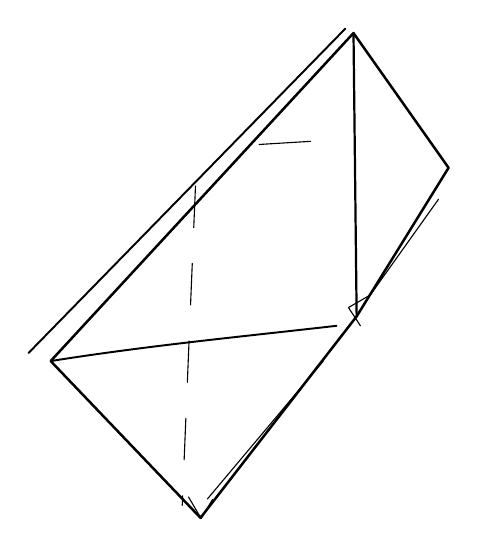
\begin{tikzpicture}[x=0.008cm,y=-0.008cm,line cap=round,line join=round]
\coordinate (T) at (581,87);
\coordinate (R) at (732,301);
\coordinate (M) at (586,537);
\coordinate (B) at (338,857);
\coordinate (L) at (100,608);
\draw[line width=0.9pt] (L)--(T)--(R)--(M)--(B)--(L);
\draw[line width=0.8pt] (T)--(M);
\draw[line width=0.7pt] (L) .. controls (257,583) and (415,568) .. (554,552);
\draw[line width=0.7pt] (65,595)--(568,80);
\draw (431,264)--(513,259);
\draw (716,351)--(597,518);
\draw (349,827)--(533,608);
\draw[dash pattern=on 15pt off 13pt] (330,330)--(309,837);
\draw (573,523)--(606,504);
\draw (573,523)--(592,552);
\draw (319,824)--(339,858)--(357,828);
\end{tikzpicture}}

\figure{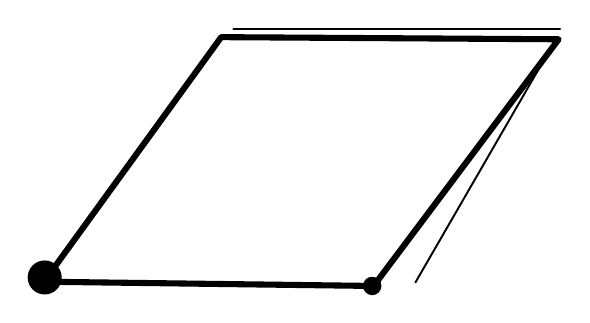
\begin{tikzpicture}[x=0.009cm,y=-0.009cm,line cap=round,line join=round]
\draw[line width=2.2pt] (83,423)--(333,78)--(809,81)--(548,429)--cycle;
\draw[line width=0.7pt] (607,424)--(789,109);
\draw[line width=0.7pt] (350,66)--(811,66);
\fill (84,417) circle (24);
\fill (546,429) circle (13);
\end{tikzpicture}}

\figure{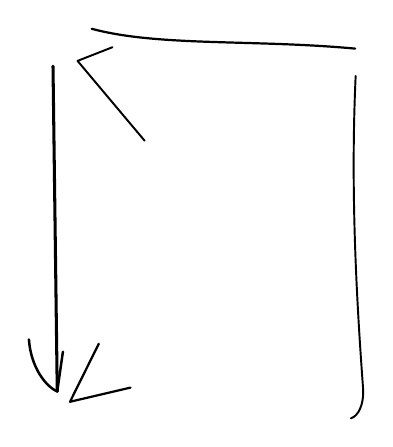
\begin{tikzpicture}[x=0.006cm,y=-0.006cm,line cap=round,line join=round]
\draw[line width=0.8pt] (224,115) .. controls (365,153) and (566,137) .. (782,157);
\draw[line width=0.7pt] (194,183)--(268,154);
\draw[line width=0.7pt] (194,183)--(336,352);
\draw[line width=1.1pt] (142,194)--(151,883);
\draw[line width=0.9pt] (91,773) .. controls (95,832) and (127,873) .. (151,883)--(163,799);
\draw[line width=0.7pt] (783,215) .. controls (773,436) and (782,652) .. (799,880)
 .. controls (800,911) and (789,935) .. (773,940);
\draw[line width=0.8pt] (239,782)--(178,905)--(306,875);
\end{tikzpicture}}

\figure{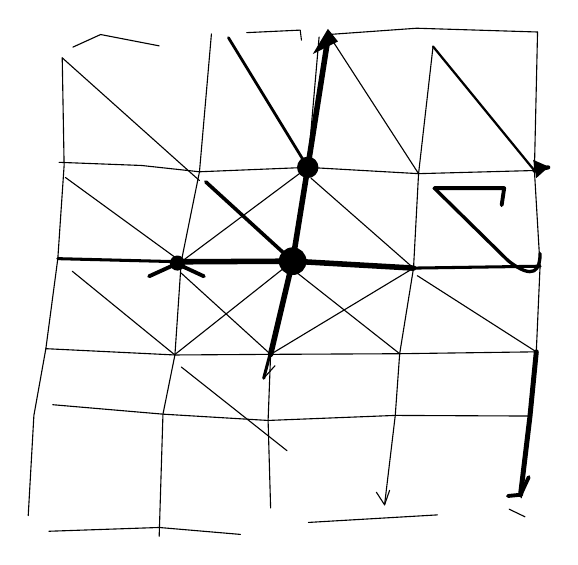
\begin{tikzpicture}[x=0.008cm,y=-0.008cm,line cap=round,line join=round]
\draw (91,83)--(94,254)--(84,402)--(65,545)--(46,651)--(37,810);
\draw (328,45)--(309,264)--(280,407)--(270,555)--(251,649)--(245,843);
\draw (499,50)--(481,257)--(457,406)--(422,554)--(418,659)--(422,798);
\draw (680,65)--(657,267)--(649,417)--(627,553)--(620,651)--(603,793);
\draw (846,42)--(841,262)--(850,414)--(844,550)--(834,652)--(820,782);
\draw (108,66)--(152,46)--(245,64);
\draw (384,43)--(469,39)--(471,55);
\draw (514,46)--(654,36)--(846,42);
\draw (86,249)--(217,254)--(309,264)--(481,257)--(657,267)--(841,262);
\draw[line width=1.1pt] (84,402)--(280,407)--(457,406)--(649,417)--(850,414);
\draw (65,545)--(270,555)--(422,554)--(627,553)--(844,550);
\draw (76,634)--(251,649)--(418,659)--(620,651)--(834,652);
\draw (70,835)--(245,829)--(374,840);
\draw (482,821)--(687,809);
\draw (801,800)--(826,812);
\draw (91,83)--(309,278);
\draw[line width=1pt] (355,51)--(481,257);
\draw (514,46)--(657,267);
\draw[line width=0.8pt] (680,65)--(841,262);
\draw (96,273)--(280,407);
\draw[line width=1.3pt] (319,280)--(457,406);
\draw (486,274)--(649,417);
\draw[line width=1.2pt] (682,290)--(799,405);
\draw (107,422)--(270,555);
\draw (280,425)--(422,554);
\draw (457,419)--(627,553);
\draw (655,429)--(844,550);
\draw (280,574)--(448,707);
\draw (280,407)--(481,257);
\draw (422,554)--(649,417);
\draw (269,555)--(457,406);
\draw[line width=2pt] (514,46)--(481,257)--(457,406)--(422,554);
\draw[line width=2pt] (280,407)--(457,406)--(649,417);
\fill (481,257) circle (17);
\fill (457,406) circle (22);
\fill (274,409) circle (12);
\fill (513,37)--(489,77)--(529,57)--cycle;
\draw[line width=1.5pt] (841,262)--(863,257);
\fill (864,256)--(839,245)--(844,274)--cycle;
\draw[line width=1.4pt] (316,430)--(273,410)--(229,430);
\draw[line width=1.1pt] (421,554)--(411,592);
\draw (411,592)--(429,572);
\draw[line width=1.4pt] (682,290)--(793,290)--(789,317);
\draw[line width=1.2pt] (799,405) .. controls (841,438) and (850,419) .. (850,394);
\draw[line width=1.8pt] (844,550)--(834,652)--(819,777);
\draw[line width=1.4pt] (799,779)--(819,777)--(832,749);
\draw (590,773)--(603,793)--(611,770);
\end{tikzpicture}}

\figure{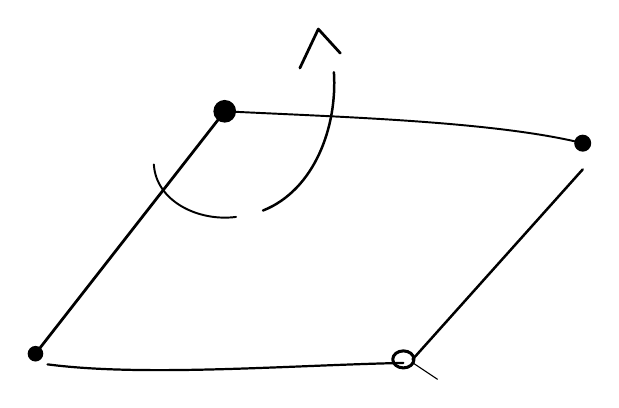
\begin{tikzpicture}[x=0.009cm,y=-0.009cm,line cap=round,line join=round]
\draw[line width=0.7pt] (332,136) .. controls (493,144) and (711,150) .. (837,181);
\draw[line width=1pt] (332,136)--(65,478);
\draw[line width=0.9pt] (837,218)--(597,486);
\draw[line width=0.8pt] (82,493) .. controls (219,511) and (428,494) .. (584,491);
\fill (332,136) circle (16);
\fill (837,181) circle (12);
\fill (65,478) circle (11);
\draw[line width=1.1pt] (584,486) ellipse (15 and 12);
\draw (596,490)--(632,514);
\draw[line width=0.7pt] (232,211) .. controls (235,263) and (295,292) .. (348,285);
\draw[line width=0.9pt] (386,276) .. controls (459,247) and (491,157) .. (486,81);
\draw[line width=1pt] (438,75)--(464,20)--(495,54);
\end{tikzpicture}}

$\unsure{\deleted{2}\inserted{4}|\deleted{4}\inserted{2}}$ carrés

$8$ arêtes

$4$ sommets

\diagram{\fbox{\begin{tikzcd}
E_{\varepsilon,+}\arrow[r,bend left,very thick]\arrow[d,shift right=.35ex,very thick]&
E_{\varepsilon,-}\arrow[l,bend left,very thick]\arrow[d,shift left=.35ex,very thick]\\
\unsure{E_Q|\overline E_Q}\arrow[u,shift right=.35ex,very thick]\arrow[r,very thick]&\unsure{E_H|\overline E_H}\arrow[u,shift left=.35ex,very thick]
\end{tikzcd}}}

\margin{22}

\scanpage{24}
\margin{Mireille \& enfants}
\figure{
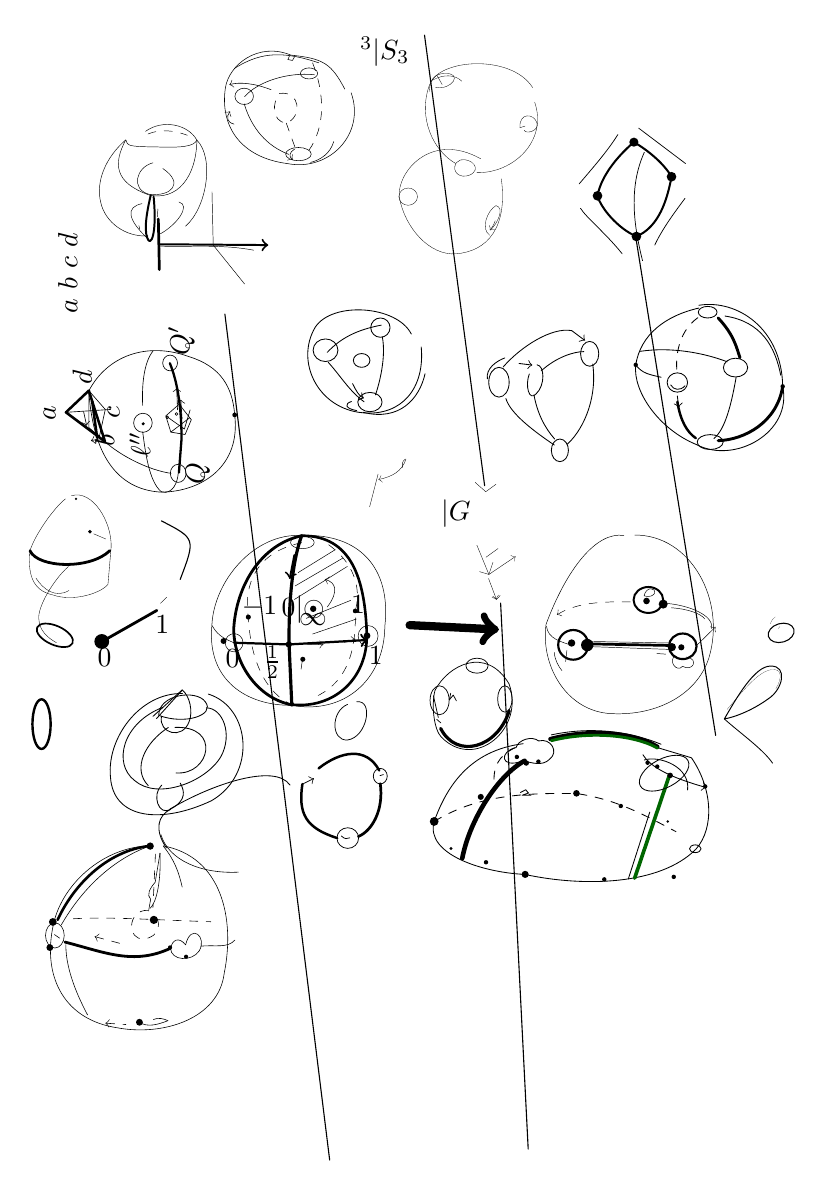
\begin{tikzpicture}[x=.007cm,y=-.007cm,line cap=round,line join=round]
\begin{scope}[shift={(212,315)},xscale={333/900},yscale={308/832},line width=0.64750000\pgflinewidth]
\draw (157,95) .. controls (96,211) and (100,304) .. (273,365) .. controls (410,393) and (503,278) .. (506,96);
\draw (158,95) .. controls (167,121) and (160,128) .. (303,129) .. controls (433,134) and (491,127) .. (506,96);
\draw (254,53) .. controls (338,-8) and (463,18) .. (506,96);
\draw[dashed] (266,66) .. controls (327,41) and (389,47) .. (460,72);
\draw (157,95) .. controls (56,183) and (11,300) .. (34,398) .. controls (55,500) and (158,572) .. (266,565);
\draw (506,96) .. controls (593,183) and (555,427) .. (450,518);
\draw (291,207) .. controls (207,228) and (181,337) .. (271,361) .. controls (381,374) and (446,307) .. (339,235);
\draw (237,407) .. controls (158,423) and (162,483) .. (270,583);
\draw (418,399) .. controls (480,414) and (405,515) .. (321,558);
\draw[line width=0.71225pt] (280,365) .. controls (266,424) and (244,527) .. (263,575) .. controls (278,622) and (312,564) .. (294,373);
\draw[line width=0.97125pt] (317,482) -- (322,730);
\draw (315,433) -- (312,472);
\draw (222,515) -- (226,532);
\draw[line width=0.71225pt,->] (320,606) -- (856,610);
\draw (323,615) .. controls (459,621) and (620,604) .. (784,635);
\draw (580,349) -- (586,610) -- (740,801);
\end{scope}
\begin{scope}[shift={(435,150)},xscale={360/900},yscale={275/688},line width=0.70000000\pgflinewidth]
\draw (581,270) .. controls (520,154) and (484,131) .. (337,116) .. controls (190,55) and (57,158) .. (40,263) .. controls (13,442) and (112,581) .. (321,608) .. controls (511,645) and (676,474) .. (610,287);
\draw (80,177) .. controls (210,93) and (317,103) .. (464,151);
\draw (426,603) .. controls (471,591) and (515,563) .. (531,508);
\draw (127,304) .. controls (187,236) and (323,192) .. (443,205);
\draw (125,337) .. controls (159,449) and (228,529) .. (327,566);
\draw[dashed] (435,151) .. controls (491,292) and (493,441) .. (419,547);
\draw[dashed] (285,290) .. controls (380,275) and (391,399) .. (314,425) .. controls (250,414) and (251,332) .. (285,290);
\draw[dashed] (316,425) -- (359,544);
\draw (125,303) ellipse (42 and 37);
\draw (419,199) ellipse (39 and 25);
\draw (371,565) ellipse (58 and 30);
\draw[->] (247,273) .. controls (174,244) and (104,237) .. (58,250);
\draw[->] (79,429) .. controls (46,421) and (43,396) .. (61,371);
\draw[->] (354,542) .. controls (329,557) and (327,575) .. (345,591);
\draw (331,118) -- (323,136) -- (344,140) -- (353,124);
\end{scope}
\node at (740,190) {\(\unsure{\circlearrowleft^{3}|\mathfrak S_3}\)};
\begin{scope}[shift={(752,196)},xscale={276/900},yscale={372/1213},line width=0.53666667\pgflinewidth]
\draw (835,193) .. controls (709,-8) and (267,21) .. (223,183) .. controls (157,373) and (246,566) .. (380,642);
\draw (847,279) .. controls (926,509) and (720,701) .. (505,696);
\draw (528,614) .. controls (235,450) and (34,690) .. (46,839) .. controls (79,1024) and (227,1188) .. (382,1176) .. controls (570,1161) and (688,1019) .. (650,733);
\draw (260,191) .. controls (355,213) and (431,102) .. (310,110) .. controls (252,111) and (227,154) .. (223,216);
\draw (270,122) -- (300,175);
\draw (241,150) .. controls (307,113) and (374,115) .. (416,155);
\draw (760,430) .. controls (754,340) and (842,344) .. (860,401) .. controls (877,449) and (795,470) .. (785,446);
\draw (760,430) -- (790,421);
\draw (383,638) .. controls (352,692) and (406,733) .. (461,711) .. controls (538,678) and (476,607) .. (408,621) -- (383,638);
\draw (99,838) ellipse (55 and 51);
\draw (581,1066) .. controls (526,1029) and (566,921) .. (618,891) .. controls (673,903) and (625,1002) .. (584,1036);
\draw[->] (614,980) .. controls (606,1003) and (593,1023) .. (583,1036);
\end{scope}
\begin{scope}[shift={(106,685)},xscale={389/900},yscale={313/724},line width=0.75638889\pgflinewidth]
\draw (225,278) .. controls (301,133) and (466,69) .. (647,135) .. controls (778,176) and (828,261) .. (837,379) .. controls (863,593) and (702,699) .. (532,703) .. controls (363,695) and (244,573) .. (225,278);
\fill (837,379) circle (10);
\draw (495,110) .. controls (455,158) and (447,258) .. (451,339);
\draw[line width=0.832028pt] (565,162) .. controls (600,247) and (614,362) .. (614,479) -- (603,621);
\draw[->] (597,357) -- (594,265);
\draw[->] (616,394) -- (611,315);
\draw (566,161) ellipse (31 and 33);
\draw (452,412) ellipse (39 and 40);
\fill (453,416) circle (7);
\draw (600,624) ellipse (33 and 38);
\draw (451,450) .. controls (462,533) and (477,658) .. (529,701) .. controls (578,716) and (598,658) .. (600,624);
\draw (290,489) .. controls (365,556) and (481,611) .. (570,624);
\draw[line width=0.907667pt] (129,368) -- (225,277) -- (293,491) -- cycle;
\draw (129,368) -- (316,356);
\draw (225,277) -- (225,432) -- (293,491);
\draw (129,368) -- (270,467) -- (294,356) -- (225,277);
\draw[line width=0.907667pt] (239,321) -- (260,475);
\draw[->] (286,476) -- (234,487);
\draw[->] (203,365) -- (216,424);
\draw (604,334) -- (548,383) -- (569,451) -- (629,461) -- (655,399) -- cycle;
\draw (548,383) -- (626,438) -- (650,358);
\draw (569,451) -- (648,391);
\draw (554,389) circle (6);
\draw (593,375) circle (6);
\node[rotate=90] at (614,69) {\(Q'\)};
\node[rotate=90] at (61,373) {\(a\)};
\node[rotate=90] at (292,485) {\(\unsure{b}\)};
\node[rotate=90] at (329,367) {\(\unsure{c}\)};
\node[rotate=90] at (197,221) {\(d\)};
\node[rotate=90] at (330,278) {\(\circlearrowleft\)};
\node[rotate=90] at (440,503) {\(\ell''\)};
\node[rotate=90] at (683,625) {\(Q\)};
\end{scope}
\begin{scope}[shift={(582,630)},xscale={902/1804},yscale={309/618},line width=0.87500000\pgflinewidth]
\draw (412,144) .. controls (359,40) and (126,25) .. (64,119) .. controls (-11,244) and (74,417) .. (238,430) .. controls (378,442) and (462,340) .. (448,191);
\draw (237,428) .. controls (370,462) and (442,378) .. (462,288);
\draw (107,211) .. controls (157,158) and (215,129) .. (303,112);
\draw (111,247) .. controls (157,298) and (188,352) .. (241,390);
\draw (307,155) .. controls (321,227) and (297,322) .. (282,365);
\draw (101,203) ellipse (45 and 41);
\draw (300,121) ellipse (35 and 35);
\draw (262,391) ellipse (44 and 35);
\draw (232,240) ellipse (30 and 25);
\draw[->] (199,324) .. controls (211,348) and (222,369) .. (240,377);
\draw (195,389) .. controls (169,397) and (171,414) .. (214,422);
\draw[->] (745,264) .. controls (809,190) and (922,118) .. (994,132) -- (1042,168);
\draw (1070,253) .. controls (1086,361) and (1047,479) .. (978,544);
\draw (931,547) .. controls (830,479) and (769,424) .. (755,378);
\draw (883,278) .. controls (937,229) and (1000,208) .. (1038,208);
\draw (857,365) .. controls (869,431) and (895,483) .. (932,525);
\draw (730,319) ellipse (37 and 54);
\draw (1059,216) ellipse (33 and 45);
\draw (951,566) ellipse (31 and 41);
\draw (840,289) .. controls (824,330) and (839,391) .. (865,361) .. controls (899,329) and (895,258) .. (868,256);
\draw[->] (803,251) -- (851,257);
\draw (688,307) .. controls (682,270) and (719,243) .. (751,231);
\draw (1455,40) .. controls (1594,17) and (1756,125) .. (1759,334) .. controls (1795,502) and (1584,618) .. (1446,545) .. controls (1311,490) and (1215,353) .. (1226,256) .. controls (1244,146) and (1333,78) .. (1455,50);
\draw (1550,79) .. controls (1682,99) and (1732,191) .. (1752,294);
\draw[line width=1.05pt] (1525,86) .. controls (1582,147) and (1591,191) .. (1604,230);
\draw (1242,207) .. controls (1355,190) and (1475,213) .. (1558,245);
\draw (1226,256) .. controls (1250,288) and (1276,291) .. (1318,301);
\draw (1590,302) .. controls (1573,398) and (1551,489) .. (1510,523);
\draw[line width=1.05pt] (1759,334) .. controls (1739,464) and (1621,528) .. (1525,531);
\draw[dashed] (1451,85) .. controls (1371,143) and (1370,247) .. (1377,290);
\draw[line width=0.875pt] (1377,390) .. controls (1388,459) and (1412,500) .. (1444,522);
\draw[->] (1377,369) -- (1382,411);
\draw (1487,65) ellipse (34 and 21);
\draw (1588,266) ellipse (44 and 34);
\draw (1377,320) ellipse (37 and 35);
\draw (1496,536) ellipse (47 and 27);
\fill (1226,256) circle (8);
\fill (1759,334) circle (8);
\draw (1353,329) .. controls (1364,348) and (1387,351) .. (1405,332);
\end{scope}
\begin{scope}[shift={(699,918)},xscale={288/900},yscale={279/872},line width=0.56000000\pgflinewidth]
\draw[->] (248,34) .. controls (225,103) and (172,133) .. (92,150);
\draw (244,34) .. controls (225,49) and (224,66) .. (228,83);
\draw (90,119) -- (42,305);
\draw (700,219) -- (758,177);
\draw (700,219) -- (640,166);
\draw[->] (650,522) -- (718,688) -- (869,586);
\draw (665,672) -- (718,688) -- (741,619);
\draw (702,590) -- (770,541);
\draw[->] (716,711) -- (761,830);
\draw (740,811) -- (761,830) -- (782,807);
\end{scope}
\node at (869,1028) {\(\unsure{\circlearrowleft|G}\)};
\begin{scope}[shift={(77,986)},xscale={288/900},yscale={322/1006},line width=0.56000000\pgflinewidth]
\draw (61,341) .. controls (89,251) and (193,102) .. (262,47);
\draw (297,29) .. controls (415,-7) and (526,177) .. (521,320) -- (503,532) .. controls (461,582) and (307,632) .. (190,591) .. controls (67,565) and (49,460) .. (61,341);
\draw[line width=1.008pt] (61,341) .. controls (107,440) and (403,449) .. (514,340);
\draw (95,496) .. controls (137,561) and (206,611) .. (282,566);
\fill (322,47) circle (7);
\fill (401,233) circle (11);
\draw (422,245) -- (490,274);
\draw (279,430) .. controls (192,507) and (104,661) .. (111,726) .. controls (115,793) and (158,832) .. (211,862);
\draw[line width=0.616pt] (202,820) ellipse [x radius=110,y radius=54,rotate=-24];
\fill (468,855) circle (42);
\draw[line width=1.008pt] (470,855) -- (780,679);
\node at (484,946) {$0$};
\node at (811,758) {$1$};
\draw (800,639) -- (836,604);
\end{scope}
\begin{scope}[shift={(406,1044)},xscale={346/900},yscale={359/934},line width=0.67277778\pgflinewidth]
\draw (477,61) .. controls (249,48) and (61,280) .. (53,486) .. controls (28,744) and (218,865) .. (430,862) .. controls (673,908) and (867,744) .. (869,489) .. controls (900,213) and (748,50) .. (477,61);
\draw[line width=1.009167pt] (478,62) .. controls (287,102) and (168,295) .. (156,502) .. controls (158,677) and (278,832) .. (431,860);
\draw[line width=1.143722pt] (477,61) .. controls (439,161) and (415,345) .. (417,570) -- (430,859);
\draw[->,line width=0.672778pt] (442,153) -- (420,266);
\draw[line width=0.941889pt] (483,62) .. controls (711,65) and (776,263) .. (784,533) .. controls (784,743) and (624,879) .. (431,859);
\draw (54,486) .. controls (83,538) and (120,551) .. (157,567);
\draw[line width=0.807333pt,->] (158,567) -- (416,575) -- (788,554);
\draw[->] (504,576) -- (579,575);
\draw[->] (675,566) -- (731,550);
\draw[dashed] (477,95) .. controls (262,139) and (202,290) .. (225,447) .. controls (236,658) and (310,806) .. (431,860);
\draw[dashed] (604,105) .. controls (742,204) and (754,334) .. (729,417) .. controls (738,645) and (665,769) .. (537,824);
\draw (442,363) -- (692,207);
\draw (446,299) -- (672,167);
\draw (460,236) -- (635,128);
\draw (498,452) -- (708,367);
\draw (528,526) -- (735,455);
\draw[->] (598,398) .. controls (654,322) and (636,282) .. (586,268);
\draw (480,94) ellipse (56 and 29);
\draw (158,567) ellipse (42 and 43);
\draw (790,535) ellipse (47 and 49);
\fill (531,407) circle (15);
\fill (225,446) circle (12);
\fill (416,575) circle (15);
\fill (482,645) circle (12);
\fill (729,417) circle (11);
\fill (785,534) circle (16);
\fill (431,858) circle (10);
\fill (108,559) circle (14);
\draw (480,647) -- (474,692);
\node at (278,397) {$-1$};
\node at (338,658) {$\frac12$};
\node at (742,389) {$1$};
\node at (826,626) {$1$};
\node at (150,640) {$0$};
\node at (530,456) {$\infty$};
\node at (484,410) {$\unsure{0|\odot}$};
\end{scope}
\begin{scope}[shift={(1013,1054)},xscale={336/900},yscale={344/921},line width=0.65333333\pgflinewidth]
\draw (430,36) .. controls (295,15) and (151,201) .. (52,467) .. controls (25,661) and (143,875) .. (346,899) .. controls (571,920) and (783,818) .. (843,630) .. controls (928,349) and (754,32) .. (483,34);
\draw (54,477) .. controls (62,537) and (120,550) .. (178,570);
\draw[line width=0.98pt] (250,562) -- (654,570);
\draw (251,575) -- (652,589);
\draw (248,550) -- (653,558);
\draw (641,366) .. controls (743,375) and (869,422) .. (856,488);
\draw (661,387) .. controls (745,393) and (804,416) .. (823,441);
\draw[dashed,<-] (105,421) .. controls (214,353) and (366,357) .. (479,359);
\draw[line width=0.718667pt] (549,349) ellipse (72 and 63);
\draw[line width=0.784pt] (184,567) ellipse (73 and 72);
\draw[line width=0.784pt] (716,574) ellipse (67 and 62);
\fill (540,354) circle (16);
\fill (621,369) circle (22);
\fill (176,558) circle (18);
\fill (252,568) circle (30);
\fill (709,579) circle (15);
\fill (663,578) circle (20);
\draw (528,329) .. controls (538,283) and (585,287) .. (580,317) .. controls (555,344) and (531,327) .. (528,329);
\draw (680,621) .. controls (642,642) and (687,705) .. (715,671) .. controls (763,701) and (798,635) .. (734,626);
\draw[->] (783,570) -- (875,480);
\draw (92,604) .. controls (95,644) and (113,671) .. (129,692);
\draw (153,594) -- (147,648);
\draw (590,609) -- (633,612);
\end{scope}
\begin{scope}[shift={(1345,1215)},xscale={151/900},yscale={290/1728},line width=0.29361111\pgflinewidth]
\draw[line width=0.381694pt] (678,173) ellipse [x radius=143,y radius=101,rotate=16];
\draw (562,75) .. controls (572,35) and (598,12) .. (615,0);
\draw (665,103) -- (647,126);
\draw[line width=0.352333pt] (64,1103) .. controls (194,877) and (394,527) .. (565,532) .. controls (750,527) and (699,781) .. (541,884) .. controls (366,1011) and (178,1083) .. (64,1103);
\draw (94,1000) .. controls (255,812) and (428,590) .. (570,571) .. controls (686,549) and (693,662) .. (620,777);
\draw[line width=0.293611pt] (64,1103) .. controls (214,1240) and (487,1433) .. (585,1581);
\end{scope}
\begin{scope}[shift={(576,1282)},xscale={421/900},yscale={358/765},line width=0.81861111\pgflinewidth]
\draw (545,142) .. controls (596,43) and (743,-32) .. (832,116) .. controls (896,289) and (700,457) .. (569,322) .. controls (542,294) and (530,203) .. (545,142);
\draw[line width=1.146056pt] (567,289) .. controls (629,411) and (788,365) .. (833,220);
\draw (563,180) ellipse (37 and 56);
\draw (708,46) ellipse (43 and 29);
\draw (816,175) ellipse (28 and 51);
\draw (539,162) -- (558,247);
\draw (552,254) -- (568,268);
\draw (606,153) -- (601,178) -- (616,160) -- (628,182);
\draw[line width=0.900472pt] (94,444) .. controls (179,377) and (279,358) .. (329,452);
\draw[line width=0.982333pt] (333,503) .. controls (347,606) and (301,686) .. (248,708);
\draw[line width=0.900472pt] (166,714) .. controls (44,675) and (14,620) .. (31,505);
\draw[->] (31,505) -- (76,483);
\draw (333,474) ellipse (27 and 30);
\draw (207,714) ellipse (42 and 40);
\draw (332,472) -- (345,468);
\draw (182,706) .. controls (196,719) and (205,718) .. (215,713);
\draw (206,196) .. controls (140,224) and (142,338) .. (206,334) .. controls (282,324) and (309,177) .. (242,186);
\end{scope}
\begin{scope}[shift={(85,1340)},xscale={505/1010},yscale={295/590},line width=0.87500000\pgflinewidth]
\draw[line width=0.875pt] (65,139) ellipse (33 and 90);
\draw (576,28) .. controls (422,25) and (301,189) .. (315,331) .. controls (325,485) and (500,502) .. (681,417) .. controls (846,322) and (825,79) .. (670,30);
\draw (505,78) .. controls (358,135) and (322,282) .. (403,344) .. controls (486,416) and (662,349) .. (716,256) .. controls (759,176) and (723,81) .. (663,80);
\draw (525,151) .. controls (442,204) and (392,300) .. (452,362);
\draw (549,151) .. controls (718,144) and (676,325) .. (553,316);
\draw (490,107) .. controls (490,31) and (626,12) .. (659,58) .. controls (697,107) and (583,143) .. (490,107);
\draw (500,111) .. controls (488,172) and (577,199) .. (601,128) .. controls (614,95) and (604,38) .. (575,15) -- (469,111);
\draw (482,119) -- (576,15);
\draw (501,360) .. controls (463,394) and (490,476) .. (533,447) .. controls (593,416) and (583,379) .. (568,353);
\draw (533,448) .. controls (487,470) and (473,522) .. (518,588);
\draw (531,447) .. controls (680,358) and (911,279) .. (966,360);
\end{scope}
\begin{scope}[shift={(116,1610)},xscale={373/900},yscale={370/893},line width=0.72527778\pgflinewidth]
\draw (478,49) .. controls (273,52) and (84,221) .. (52,410) .. controls (10,633) and (110,811) .. (334,845) .. controls (536,883) and (779,806) .. (803,606) .. controls (851,369) and (793,97) .. (536,49);
\draw[line width=0.942861pt] (478,49) .. controls (283,71) and (139,229) .. (74,373);
\draw (478,49) .. controls (308,110) and (176,245) .. (90,395);
\draw[line width=1.015389pt] (106,470) .. controls (279,514) and (406,573) .. (568,497);
\draw (110,481) .. controls (109,600) and (173,728) .. (205,789);
\draw (62,441) ellipse (41 and 55);
\draw (634,482) .. controls (658,384) and (729,448) .. (694,508) .. controls (661,558) and (570,552) .. (568,497) .. controls (576,460) and (604,445) .. (634,482);
\draw (700,488) .. controls (763,481) and (816,499) .. (850,461);
\draw[dashed] (143,368) .. controls (301,359) and (471,372) .. (744,381);
\draw[dashed] (470,331) .. controls (377,327) and (377,465) .. (451,455) .. controls (524,453) and (531,368) .. (492,352);
\draw[dashed,<-] (236,446) -- (374,483);
\draw[dashed] (502,85) -- (491,319);
\draw (522,81) -- (501,208) .. controls (477,236) and (462,263) .. (481,283) -- (472,334);
\draw (522,81) .. controls (527,200) and (508,295) .. (479,322);
\draw (537,51) .. controls (586,111) and (605,167) .. (619,229);
\draw (526,0) .. controls (560,113) and (704,172) .. (865,164);
\draw (433,822) .. controls (470,844) and (511,831) .. (555,815);
\draw (493,809) .. controls (515,799) and (536,805) .. (557,814);
\draw[dashed,<-] (283,825) -- (373,831);
\fill (479,50) circle (16);
\fill (53,382) circle (17);
\fill (40,494) circle (15);
\fill (495,373) circle (18);
\fill (432,821) circle (15);
\fill (636,534) circle (9);
\fill (566,493) circle (9);
\draw (60,437) -- (83,453);
\end{scope}
\begin{scope}[shift={(814,1410)},xscale={526/1052},yscale={309/618},line width=0.87500000\pgflinewidth]
\draw (354,70) .. controls (156,95) and (75,230) .. (31,352) .. controls (-3,471) and (207,537) .. (359,544) .. controls (572,590) and (849,584) .. (980,453) .. controls (1050,374) and (1039,230) .. (964,121) -- (840,84);
\draw[line width=1.4875pt] (452,53) .. controls (590,16) and (752,26) .. (841,81);
\draw[green!40!black,line width=1.05pt] (456,59) .. controls (590,25) and (752,36) .. (841,86);
\draw (456,38) .. controls (616,4) and (752,31) .. (854,72);
\draw[line width=1.6625pt] (133,485) .. controls (160,345) and (262,185) .. (359,132);
\draw[green!40!black,line width=1.3125pt] (758,558) -- (885,182);
\draw (735,561) -- (813,318);
\draw (354,132) .. controls (268,164) and (267,97) .. (328,84) .. controls (336,56) and (385,40) .. (410,60) .. controls (453,48) and (485,99) .. (450,126) .. controls (424,153) and (384,139) .. (354,132);
\draw (865,177) ellipse [x radius=98,y radius=52,rotate=28];
\draw[->] (788,110) .. controls (812,148) and (868,187) .. (1018,229);
\draw (793,129) .. controls (849,112) and (961,154) .. (950,238);
\draw[dashed] (31,352) .. controls (178,263) and (330,247) .. (549,251) .. controls (690,272) and (785,324) .. (908,389);
\draw[dashed] (248,199) .. controls (248,132) and (286,104) .. (323,85);
\draw (344,247) -- (363,237) -- (373,249) -- (350,257) -- (382,257);
\fill (31,352) circle (16);
\fill (200,263) circle (11);
\fill (547,250) circle (12);
\fill (708,296) circle (8);
\fill (878,352) circle (5);
\fill (92,450) circle (6);
\fill (219,500) circle (8);
\fill (361,544) circle (13);
\fill (648,562) circle (8);
\fill (900,553) circle (8);
\draw (978,451) ellipse (21 and 14);
\fill (331,118) circle (8);
\fill (365,140) circle (10);
\fill (409,135) circle (8);
\fill (805,139) circle (8);
\fill (840,153) circle (8);
\fill (887,185) circle (10);
\fill (1014,225) circle (8);
\end{scope}
\begin{scope}[shift={(1081,569)},rotate=90,xscale={549/1191},yscale={415/900},line width=0.80667506\pgflinewidth]
\draw[line width=0.726008pt] (95,250) .. controls (126,178) and (206,110) .. (255,97) .. controls (341,112) and (424,190) .. (466,240) .. controls (434,296) and (381,359) .. (330,388) .. controls (210,366) and (128,326) .. (95,250);
\draw (0,274) .. controls (139,239) and (289,219) .. (426,281);
\fill (95,250) circle (19);
\fill (255,97) circle (19);
\fill (466,240) circle (18);
\fill (330,388) circle (19);
\draw (27,194) .. controls (107,130) and (169,53) .. (206,30);
\draw (302,25) .. controls (360,74) and (431,137) .. (496,177);
\draw (521,259) -- (382,443);
\draw (61,322) .. controls (128,353) and (199,407) .. (245,441);
\end{scope}
\draw (812,160)--(921,977);
\draw (450,666)--(640,2200);
\draw (335,1041) .. controls (397,1073) .. (369,1147);
\draw (1195,526)--(1340,1430);
\draw[->,line width=3pt] (785,1230)--(947,1238);
\draw (950,1190)--(1000,2180);
\node[rotate=90] at (165,592) {\(a\ b\ c\ d\)};
\end{tikzpicture}
}% crop-candidate: scan 24
\margin{\(\operatorname{diag}_Q\simeq\omega_Q\)\quad
\(\operatorname{diag}_Q\wedge\omega_Q\simeq\operatorname{codiag}_Q\)}
\margin{\deleted{\unsure{avec} un ens à trois éléments on fait \(3\times2=6\) \unsure{cartes} \unsure{elliptiques} de type \((1,1)\)}}
avec un ens \(I\) de card \(4\),
on peut trouver \(\unsure{1\deleted{4}\inserted{7}|1\deleted{7}\inserted{4}}\) \unsure{ponts|points} \unsure{on|ou|or} canoniques \inserted{de type \((0,4)\)}
\((14=3\times4+\deleted{3\times}2)\)
dont deux tétraédrales,
\deleted{\unsure{quatre}}\inserted{trois} carrés, \deleted{deux} \(2\times3=6\)
assemblages de \deleted{\unsure{F}} ``\(J\)'' droits,
\(6=2\times3\) assemblages de \inserted{\(1\)} \(J\) gauches.
\margin{23}

\scanpage{25}

\figure{\begin{tikzpicture}[x=.009cm,y=-.009cm,line cap=round,
 every node/.style={inner sep=0pt,anchor=west,font=\small}]
% One table: the descriptors and the mathematical labels share their manuscript rows.
\node[anchor=center,font=\Large] at (264,65) {$A$};
\node at (320,72) {triangle};
\node[anchor=center,font=\Large] at (246,143) {$\vec T$};
\node at (306,153) {tétraèdre orienté};
\node[anchor=center,font=\Large] at (246,229) {$\overset{\deleted{\rightarrow}}{Q}$};
\node at (304,238) {carré};
\node at (419,236) {\deleted{orienté}};
\node[anchor=center,font=\Large] at (253,305) {$\unsure{\bar Q|\bar R}$};
\node at (320,311) {\deleted{hexagone}};
\node at (514,306) {carré orienté};
\node[anchor=center,font=\Large] at (262,376) {$\bar H$};
\node at (382,389) {hexagone orienté};

\node[font=\Large] at (883,67) {$\Sigma_A$};
\node[anchor=north west,font=\Large] at (880,111) {
  \begin{tikzcd}[row sep=5pt,column sep=0pt]
  \Sigma_T \arrow[d,leftrightarrow,bend left=45,start anchor=east,end anchor=east]\\
  \Sigma_Q
  \end{tikzcd}};
\node[font=\Large] at (905,300) {$E_{\vec Q}$};
\node[font=\Large] at (908,376) {$E_{\vec H}$};
\node[font=\Large] at (1107,78) {$(0,3)$};
\node[font=\Large] at (1097,158) {$(0,4)$};
\node[font=\Large] at (1106,302) {$(1,1)$};
\node[font=\Large] at (1086,485) {$(0,5)$};
\node[font=\Large] at (1085,588) {$(1,\text{\raisebox{0.6ex}{\(2\)}})$};
% Closing brace over Sigma_Q, E_{vec Q}, E_{vec H}.
\draw[line width=.45pt] (1086,220)
 .. controls (1106,211) and (1100,237) .. (1094,265)
 .. controls (1087,294) and (1095,306) .. (1110,309)
 .. controls (1094,311) and (1091,325) .. (1095,352)
 .. controls (1101,380) and (1098,400) .. (1086,406);
% Separator and closing dimension braces, with the labels to their right.
\draw[line width=.4pt] (1340,41) -- (1335,637);
\node[font=\Large] at (1371,77) {$d=0$};
\node[font=\Large] at (1375,154) {$d=1$};
\draw[line width=.45pt] (1354,145)
 .. controls (1365,150) and (1360,185) .. (1356,222)
 .. controls (1351,264) and (1357,282) .. (1377,286)
 .. controls (1357,289) and (1356,315) .. (1359,354)
 .. controls (1364,392) and (1364,408) .. (1352,411);
\draw[line width=.45pt] (1354,467)
 .. controls (1368,462) and (1357,489) .. (1354,511)
 .. controls (1351,531) and (1359,540) .. (1372,539)
 .. controls (1356,543) and (1357,564) .. (1361,585)
 .. controls (1367,607) and (1361,617) .. (1353,619);
\node[font=\Large] at (1392,530) {$d=2$};

% Two blank name slots, aligned with the last two ordered pairs.
\draw[line width=.3pt] (291,535) .. controls (304,530) and (316,530) .. (327,534);
\draw[line width=.3pt] (360,531) .. controls (375,525) and (389,529) .. (401,530);
\draw[line width=.3pt] (424,527) .. controls (450,521) and (477,517) .. (496,524);
\draw[line width=.3pt] (527,522) .. controls (547,511) and (570,516) .. (589,516);
\draw[line width=.3pt] (607,519) .. controls (654,509) and (697,504) .. (719,501)
 .. controls (733,501) and (744,503) .. (754,503);
\draw[line width=.3pt] (307,645) .. controls (323,638) and (341,640) .. (354,644);
\draw[line width=.3pt] (370,644) .. controls (390,637) and (404,647) .. (425,642)
 .. controls (451,630) and (466,643) .. (497,635)
 .. controls (535,623) and (557,631) .. (588,626)
 .. controls (624,615) and (646,619) .. (679,612)
 -- (808,598);
\draw[line width=.35pt] (726,875) .. controls (736,874) and (743,876) .. (751,878);

% Quadrilateral with four marked vertices and four unlabelled exterior edges.
\draw[line width=.7pt] (993,881) -- (1073,683) -- (1197,780) -- (1126,962) -- cycle;
\draw[line width=.7pt] (1073,683) -- (1046,552);
\draw[line width=.7pt] (1197,780) -- (1344,717);
\draw[line width=.7pt] (993,881) -- (854,929);
\draw[line width=.7pt] (1126,962) .. controls (1139,985) and (1142,1034) .. (1163,1101);
\foreach \x/\y in {993/881,1073/683,1197/780,1126/962}
 {\fill (\x,\y) circle (2pt);}
\end{tikzpicture}}

\margin{24}

\scanpage{26}
\diagram{\begin{tikzcd}[column sep=large]
\begin{gathered}\text{Carte cellulaire (pas orientée) }\text{conn}\\
\text{dont tous les sommets \unsure{sont}}\\
\text{d'ordre }3\ \inserted{\text{ou }1}
\end{gathered}
\arrow[r,leftarrow,shift left=.6ex]\arrow[r,shift right=.6ex] & \text{carte }\uline{\text{cellulaire}}
\end{tikzcd}}
\inserted{\(\mathrm{or}^{t}\)}\,/\,triangulée \(\simeq\)
\margin{\unsure{\(\deleted{\mathbf Z}n-\)|\(\deleted{\mathbf Z/n}\)}}
\unsure{revêtements|\deleted{revêtements}} de \(\mathbb P^1_{\mathbb C}\) ramifiés \unsure{seulement} en \(0,1,\infty\),
\figure{
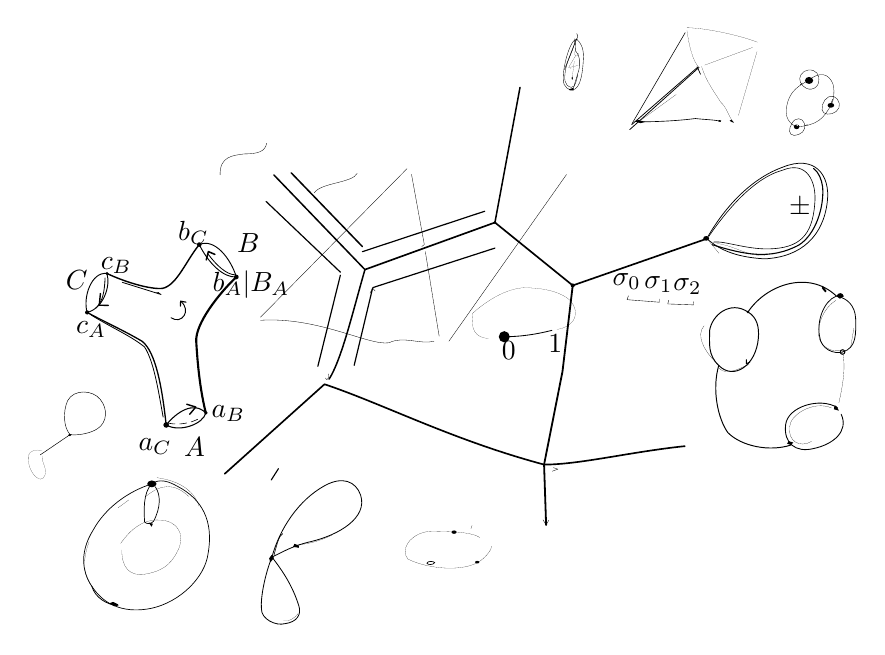
\begin{tikzpicture}[x=.0065cm,y=-.0065cm,line cap=round,line join=round]
\begin{scope}[shift={(1078,80)},line width=0.16250000\pgflinewidth]
\draw[line width=0.13pt] (40,21) .. controls (31,20) and (20,48) .. (15,78)
 .. controls (11,108) and (14,117) .. (31,120)
 .. controls (48,119) and (52,83) .. (53,55)
 .. controls (53,37) and (47,27) .. (40,21);
\draw[line width=0.11375pt] (36,20) .. controls (37,38) and (22,58) .. (18,80)
 .. controls (15,99) and (15,111) .. (29,115)
 .. controls (39,114) and (38,101) .. (42,91);
\draw[line width=0.1625pt] (16,80) .. controls (23,62) and (32,38) .. (40,20);
\draw[line width=0.14625pt] (40,10) .. controls (44,15) and (39,23) .. (37,24);
\draw[line width=0.13pt] (38,24)--(37,43) .. controls (47,52) and (47,70) .. (44,81)
 .. controls (40,94) and (36,107) .. (33,118);
\draw (37,43) .. controls (32,55) and (43,58) .. (43,48);
\draw (26,76)--(43,72);
\draw (37,54)--(24,76)--(29,78);
\draw (35,64)--(31,96);
\fill (31,97) ellipse (1.3 and 3.3);
\fill (33,116)--(34,121)--(27,121)--(24,119)--cycle;
\end{scope}
\begin{scope}[shift={(1210,65)},xscale={280/900},yscale={226/726},line width=0.25277778\pgflinewidth]
\draw[line width=0.202222pt] (51,645)--(385,74);
\draw (396,43) .. controls (510,45) and (708,85) .. (840,134);
\draw (396,61) .. controls (409,156) and (432,252) .. (471,292);
\draw (507,278)--(808,167);
\draw (836,193)--(719,594);
\draw (488,286) .. controls (518,387) and (582,466) .. (608,511)
 .. controls (645,541) and (659,602) .. (687,637);
\draw[line width=0.2275pt] (80,634) .. controls (249,634) and (381,622) .. (449,613)
 .. controls (509,620) and (557,620) .. (606,629);
\draw[line width=0.278056pt] (49,651)--(461,293);
\draw[line width=0.278056pt] (36,683)--(472,292);
\draw (111,620)--(330,461);
\draw[line width=0.252778pt] (460,288)--(481,335);
\fill (67,631)--(89,622)--(135,634)--(105,642)--cycle;
\fill (675,620)--(692,639)--(679,636)--(664,627)--cycle;
\fill (596,623)--(611,625)--(607,634)--(593,632)--cycle;
\end{scope}
\begin{scope}[shift={(1515,150)},xscale={131/900},yscale={150/1031},line width=0.13515873\pgflinewidth]
\draw[line width=0.108127pt] (389,212) .. controls (520,101) and (658,105) .. (718,283)
 .. controls (729,376) and (729,470) .. (685,548)
 .. controls (582,725) and (510,817) .. (225,840)
 .. controls (78,777) and (58,654) .. (107,493)
 .. controls (155,354) and (245,288) .. (389,212);
\draw[line width=0.121643pt] (274,243) .. controls (241,177) and (292,81) .. (384,75)
 .. controls (484,72) and (537,134) .. (518,240)
 .. controls (505,333) and (363,392) .. (274,243);
\draw[line width=0.121643pt] (716,430) .. controls (622,414) and (557,514) .. (565,611)
 .. controls (571,677) and (686,691) .. (755,632)
 .. controls (825,577) and (808,469) .. (716,430);
\draw[line width=0.121643pt] (160,793) .. controls (203,703) and (303,717) .. (328,792)
 .. controls (352,895) and (287,944) .. (189,954)
 .. controls (114,953) and (113,864) .. (160,793);
\fill (390,216) ellipse (55 and 47);
\fill (683,550) ellipse (45 and 32);
\fill (223,839) ellipse (38 and 31);
\fill[white] (232,821) ellipse (9 and 8);
\draw[line width=0.148675pt] (270,278)--(298,252);
\draw[line width=0.148675pt] (687,515)--(709,468);
\draw[line width=0.135159pt] (368,810)--(330,826);
\end{scope}
\begin{scope}[shift={(112,468)},xscale={410/900},yscale={459/1008},line width=0.42301587\pgflinewidth]
\coordinate (cB) at (193,199);
\coordinate (cA) at (108,366);
\coordinate (bC) at (589,75);
\coordinate (bA) at (748,214);
\coordinate (aC) at (447,849);
\coordinate (aB) at (617,797);
\draw[line width=0.507619pt] (cB) .. controls (269,235) and (377,268) .. (431,263)
 .. controls (493,250) and (533,143) .. (bC);
\draw[line width=0.761429pt] (bA) .. controls (678,280) and (570,414) .. (576,492)
 .. controls (584,628) and (598,720) .. (aB);
\draw[line width=0.465317pt] (cA) .. controls (178,404) and (270,446) .. (344,490)
 .. controls (402,536) and (429,684) .. (aC);
\draw[line width=0.296111pt] (125,377) .. controls (221,436) and (291,464) .. (354,514)
 .. controls (395,577) and (414,706) .. (434,815);
\draw[line width=0.338413pt] (cB) .. controls (126,190) and (89,302) .. (cA)
 .. controls (176,350) and (210,254) .. (cB);
\draw[line width=0.296111pt] (185,218) .. controls (182,286) and (173,320) .. (146,347);
\draw[line width=0.507619pt] (165,285)--(160,335)--(199,336);
\draw[line width=0.338413pt] (bC) .. controls (655,46) and (724,135) .. (bA)
 .. controls (692,218) and (627,153) .. (bC);
\draw[line width=0.296111pt] (627,116) .. controls (663,164) and (705,204) .. (744,205);
\draw[line width=0.549921pt] (619,141)--(628,105)--(656,117);
\draw[line width=0.380714pt] (aC) .. controls (490,796) and (562,744) .. (aB)
 .. controls (607,844) and (506,883) .. (aC);
\draw[dash pattern=on 2.538095pt off 1.692063pt,line width=0.211508pt] (455,841) .. controls (502,851) and (553,841) .. (589,821);
\draw[line width=0.507619pt] (535,760)--(574,772)--(548,803);
\fill (cB) circle (7);
\fill (cA) circle (9);
\fill (bC) circle (10);
\fill (bA) circle (10);
\fill (aC) circle (12);
\fill (aB) circle (8);
\node at (64,227) {$C$};
\node at (233,166) {$c_B$};
\node at (125,441) {$c_A$};
\node at (564,25) {$b_C$};
\node at (799,67) {$B$};
\node at (811,247) {$\unsure{b_A|B_A}$};
\node at (714,800) {$a_B$};
\node at (400,943) {$a_C$};
\node at (568,943) {$A$};
\draw[line width=0.338413pt] (468,389) .. controls (513,420) and (558,358) .. (509,318);
\draw[line width=0.423016pt] (508,339)--(509,318)--(532,322);
\draw[line width=0.296111pt] (259,237)--(425,289);
\fill (425,289)--(414,279)--(403,281)--cycle;
\end{scope}
\begin{scope}[shift={(420,185)},line width=0.54166667\pgflinewidth]
\draw (1,181) .. controls (0,144) and (27,143) .. (48,140)
 .. controls (76,140) and (89,135) .. (92,119);
\draw (185,216) .. controls (198,196) and (259,197) .. (269,178);
\draw[line width=0.541667pt] (106,181)--(284,366);
\draw[line width=0.541667pt] (140,177)--(279,321);
\draw[line width=0.433333pt] (91,233)--(236,371);
\draw[line width=0.595833pt] (284,366)--(538,274);
\draw[line width=0.433333pt] (279,331)--(518,252);
\draw[line width=0.433333pt] (300,401)--(538,324);
\draw[line width=0.541667pt] (284,366) .. controls (260,449) and (239,540) .. (214,580);
\draw[line width=0.433333pt] (236,377)--(192,555);
\draw[line width=0.433333pt] (299,402)--(263,553);
\draw (294,412)--(299,402)--(304,408);
\draw (213,570) .. controls (214,580) and (209,584) .. (207,578);
\draw[line width=0.541667pt] (538,274)--(587,10);
\draw[line width=0.595833pt] (538,274)--(690,397)--(951,306);
\fill (538,274) circle (3);
\fill (690,397) circle (4);
\draw[line width=0.65pt] (690,397)--(670,565)--(634,747)--(638,865);
\draw (632,855)--(638,865)--(643,856);
\draw (652,753)--(661,756)--(650,760);
\draw[line width=0.595833pt] (10,765)--(205,590)
 .. controls (321,629) and (455,699) .. (634,747)
 .. controls (704,747) and (803,722) .. (909,711);
\draw (80,459)--(366,169);
\draw (375,180)--(400,317)--(395,321);
\draw (402,331)--(429,496);
\draw (80,465) .. controls (194,458) and (291,515) .. (331,509)
 .. controls (359,495) and (393,513) .. (419,506);
\draw (448,506)--(678,180);
\end{scope}
\begin{scope}[shift={(1355,325)},xscale={273/900},yscale={215/709},line width=0.24645833\pgflinewidth]
\draw[line width=0.271104pt] (56,545) .. controls (161,359) and (329,163) .. (546,85)
 .. controls (746,4) and (854,129) .. (832,310)
 .. controls (806,526) and (668,665) .. (427,676)
 .. controls (256,666) and (142,624) .. (56,545);
\draw[line width=0.221812pt] (69,531) .. controls (179,371) and (356,155) .. (544,105)
 .. controls (700,40) and (766,179) .. (751,324)
 .. controls (735,529) and (650,607) .. (456,612)
 .. controls (309,615) and (166,558) .. (99,568);
\draw[line width=0.394333pt] (91,585) .. controls (297,649) and (465,685) .. (649,587)
 .. controls (758,519) and (813,340) .. (802,212)
 .. controls (795,164) and (777,118) .. (744,94);
\draw (118,576) .. controls (249,595) and (324,664) .. (430,653);
\draw (56,545)--(135,641);
\fill (52,544) ellipse (19 and 15);
\node at (655,347) {$\pm$};
\end{scope}
\begin{scope}[shift={(1182,542)},xscale={187/900},yscale={89/428},line width=0.16881944\pgflinewidth]
\node at (161,158) {$\sigma_0$};
\node at (459,182) {$\sigma_1$};
\node at (733,199) {$\sigma_2$};
\draw[line width=0.135056pt] (177,290)--(165,326)--(470,350)--(469,320);
\draw[line width=0.135056pt] (555,331)--(548,366)--(789,375)--(790,345);
\end{scope}
\begin{scope}[shift={(907,574)},xscale={225/900},yscale={155/620},line width=0.20312500\pgflinewidth]
\draw (152,447) .. controls (43,438) and (16,370) .. (29,250)
 .. controls (180,115) and (352,32) .. (492,52)
 .. controls (645,59) and (766,108) .. (806,167)
 .. controls (884,286) and (783,364) .. (688,376);
\draw[line width=0.304688pt] (277,433) .. controls (424,432) and (550,408) .. (649,383);
\fill (277,433) ellipse (43 and 44);
\node at (313,540) {$0$};
\node at (675,490) {$1$};
\end{scope}
\begin{scope}[shift={(1342,552)},xscale={338/900},yscale={370/985},line width=0.34873016\pgflinewidth]
\draw[line width=0.34873pt] (294,218) .. controls (389,75) and (610,-2) .. (754,135);
\draw (786,426) .. controls (806,511) and (782,622) .. (767,690);
\draw[line width=0.34873pt] (142,496) .. controls (105,622) and (138,775) .. (190,846)
 .. controls (261,917) and (407,946) .. (517,910);
\draw[line width=0.34873pt] (294,218) .. controls (202,156) and (106,233) .. (94,316)
 .. controls (95,383) and (84,441) .. (142,496)
 .. controls (218,574) and (336,499) .. (348,354)
 .. controls (353,297) and (341,245) .. (294,218);
\draw (66,289) .. controls (21,340) and (68,421) .. (123,476);
\draw (143,510) .. controls (186,555) and (253,507) .. (300,491);
\draw[line width=0.278984pt] (754,135) .. controls (686,161) and (652,268) .. (666,341)
 .. controls (673,414) and (743,438) .. (786,426)
 .. controls (859,405) and (856,333) .. (854,250)
 .. controls (851,187) and (813,146) .. (754,135);
\draw (751,158) .. controls (665,210) and (634,350) .. (688,393)
 .. controls (724,424) and (762,424) .. (792,415);
\draw (845,302)--(828,402);
\draw[line width=0.313857pt] (759,715) .. controls (667,659) and (500,711) .. (490,804)
 .. controls (478,899) and (541,952) .. (636,928)
 .. controls (740,906) and (819,837) .. (779,750);
\draw (729,717) .. controls (633,676) and (511,755) .. (511,815)
 .. controls (500,889) and (563,927) .. (625,891);
\fill (294,218) circle (7);
\fill (754,135) .. controls (765,113) and (786,116) .. (793,136)
 --(772,149)--cycle;
\draw[line width=0.34873pt] (786,426) circle (12);
\fill (759,715) .. controls (749,701) and (743,698) .. (741,724)
 --(767,731)--cycle;
\fill (517,910)--(497,902)--(507,890)--(530,897)--cycle;
\fill (683,82)--(703,109)--(696,116)--(678,94)--cycle;
\draw[line width=0.34873pt] (286,466)--(286,487)--(304,478);
\end{scope}
\begin{scope}[shift={(40,778)},xscale={175/900},yscale={194/998},line width=0.18055556\pgflinewidth]
\draw[line width=0.1625pt] (452,491) .. controls (386,419) and (378,262) .. (427,150)
 .. controls (491,30) and (680,41) .. (755,137)
 .. controls (834,232) and (824,367) .. (730,430)
 .. controls (658,478) and (537,501) .. (452,491);
\draw[line width=0.180556pt] (452,491)--(153,694);
\draw (171,656) .. controls (112,631) and (42,653) .. (32,704)
 .. controls (26,777) and (54,878) .. (118,923)
 .. controls (172,964) and (207,916) .. (206,853)
 .. controls (197,787) and (160,748) .. (174,706);
\fill (443,484)--(469,492)--(451,506)--(432,499)--cycle;
\end{scope}
\begin{scope}[shift={(142,947)},xscale={272/900},yscale={279/923},line width=0.28063492\pgflinewidth]
\draw[line width=0.252571pt] (482,75) .. controls (327,124) and (181,231) .. (103,373)
 .. controls (19,507) and (25,635) .. (94,737)
 .. controls (182,874) and (325,911) .. (481,879)
 .. controls (662,839) and (827,681) .. (846,522)
 .. controls (881,320) and (811,174) .. (646,90)
 .. controls (590,58) and (531,39) .. (482,75);
\draw (515,35) .. controls (648,54) and (752,110) .. (787,219);
\draw[line width=0.280635pt] (94,738) .. controls (116,811) and (189,855) .. (264,863);
\draw (76,449) .. controls (26,590) and (45,674) .. (97,744);
\draw (280,460) .. controls (344,371) and (422,302) .. (529,309)
 .. controls (646,310) and (704,400) .. (648,511)
 .. controls (598,607) and (541,641) .. (435,659)
 .. controls (339,674) and (286,615) .. (288,502);
\draw[line width=0.252571pt] (482,75) .. controls (424,130) and (431,251) .. (435,321)
 .. controls (447,337) and (476,335) .. (493,317)
 .. controls (540,227) and (540,147) .. (505,95);
\draw (444,155) .. controls (543,75) and (626,68) .. (722,157);
\fill (482,75) ellipse (30 and 22);
\fill (462,325)--(480,352)--(489,333)--cycle;
\fill (207,847)--(231,838)--(266,855)--(238,866)--cycle;
\draw (263,230)--(333,179);
\end{scope}
\begin{scope}[shift={(485,950)},xscale={225/900},yscale={312/1248},line width=0.27083333\pgflinewidth]
\draw[line width=0.297917pt] (149,651) .. controls (210,427) and (359,204) .. (561,93)
 .. controls (700,16) and (805,59) .. (842,166)
 .. controls (900,345) and (670,478) .. (457,529)
 .. controls (317,561) and (250,602) .. (149,651);
\draw[line width=0.216667pt] (166,632) .. controls (191,539) and (206,483) .. (233,468);
\draw (337,554) .. controls (430,553) and (524,524) .. (619,479);
\draw[line width=0.297917pt] (149,651) .. controls (96,782) and (59,965) .. (67,1056)
 .. controls (65,1134) and (178,1192) .. (252,1171)
 .. controls (345,1159) and (381,1098) .. (360,1034)
 .. controls (310,872) and (229,754) .. (149,651);
\draw (238,1148) .. controls (288,1158) and (331,1123) .. (353,1093);
\fill (147,633)--(127,662)--(137,692)--(165,658)--cycle;
\fill (325,547)--(314,571)--(359,578)--(360,562)--cycle;
\end{scope}
\begin{scope}[shift={(765,1038)},xscale={377/900},yscale={127/303},line width=0.30253086\pgflinewidth]
\draw (389,87) .. controls (355,56) and (164,54) .. (132,62)
 .. controls (54,83) and (23,146) .. (54,187)
 .. controls (126,225) and (284,252) .. (378,205)
 .. controls (410,188) and (444,149) .. (445,128);
\fill (270,62) ellipse (12 and 8);
\draw[line width=0.242025pt] (143,207) .. controls (149,195) and (173,197) .. (180,204)
 .. controls (173,215) and (149,216) .. (143,207);
\fill (378,202) ellipse (10 and 6);
\draw (349,46)--(354,31);
\end{scope}
\draw (521,962)--(535,940);
\end{tikzpicture}
}% crop-candidate: scan 26
\deleted{\unsure{variétés|variété} \unsure{algébriques|algébrique} d}
\[
\sigma_0^{\unsure{2|1}}=\sigma_1^2=\sigma_2^{\unsure{2|1}}=(\sigma_0\sigma_2)^2=(\sigma_0\sigma_1)^3=1
\]
\(\mathbb R\)-\unsure{courbes|courbe} \unsure{algébriques|algébrique}
\margin{\(\sigma_0,\sigma_1,\sigma_2\)\quad ses pts fixes}
\margin{25}

\scanpage{27}
\figure{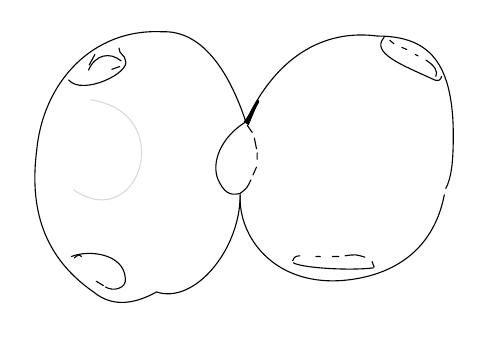
\begin{tikzpicture}[x=.009cm,y=-.009cm,line cap=round]
\draw (437,240) .. controls (407,150) and (365,111) .. (319,113)
 .. controls (220,108) and (151,185) .. (142,280)
 .. controls (130,373) and (159,436) .. (222,480)
 .. controls (251,504) and (284,495) .. (311,480)
 .. controls (364,498) and (429,421) .. (429,343);
\draw (437,240) .. controls (483,140) and (555,110) .. (622,119)
 .. controls (699,119) and (735,159) .. (729,286)
 .. controls (728,309) and (724,325) .. (719,334);
\draw (717,343) .. controls (701,425) and (640,459) .. (571,464)
 .. controls (475,470) and (426,401) .. (429,343);
\draw (437,240) .. controls (400,263) and (388,299) .. (398,322)
 .. controls (406,339) and (414,345) .. (429,341);
\draw (439,245)--(446,255) (449,263)--(452,278)
 (453,284)--(453,293) (452,304)--(447,315);
\draw (444,322) .. controls (439,333) .. (429,341);
\draw[line width=1.1pt] (454,211)--(438,240);
\fill (434,240)--(441,245)--(455,211)--cycle;
\draw (187,181) .. controls (207,204) and (276,170) .. (267,153)
 .. controls (267,146) and (258,145) .. (258,136);
\draw (215,167) .. controls (225,145) and (245,141) .. (261,154);
\draw (248,166)--(259,162) (216,160)--(224,145);
\draw (191,430) .. controls (216,420) and (265,426) .. (267,461)
 .. controls (269,475) and (250,480) .. (239,473);
\draw (195,432)..controls (201,427)..(205,430) (226,465)--(236,471);
\draw (632,121) .. controls (612,143) and (660,161) .. (699,179)
 .. controls (710,185) and (712,180) .. (713,176);
\draw (640,125)--(646,130) (657,135)--(664,138)
 (676,145)--(680,147);
\draw (691,153) .. controls (704,161) and (708,169) .. (705,176);
\draw (504,439) .. controls (519,447) and (589,450) .. (617,446);
\draw (503,436) .. controls (506,430) .. (513,429);
\draw (536,430)--(542,430) (559,430)--(568,430)
 (577,429) .. controls (592,427) .. (605,431) (615,437)--(618,445);
\draw[gray!30] (218,209) .. controls (342,227) and (287,400) .. (194,336);
\end{tikzpicture}}
\diagram{\begin{tikzcd}[column sep=large]
\left.\begin{array}{l}
4\text{ hexagones}\\16\text{ arêtes}\\10\text{ sommets}
\end{array}\right\}
\arrow[r,Rightarrow] &
\begin{array}{l}8\text{ hexagones}\\82\text{ arêtes}\\16\text{ sommets}\end{array}
\\
\begin{array}{l}(\text{dont }4\text{ ramifiés})\\\text{d'ordre}\end{array}&
\end{tikzcd}}
\begin{gather*}
\unsure{2|\deleted{6}\inserted{2}}\text{ hexag.}\\9\text{ arêtes}\\6\text{ sommets}
\end{gather*}
\figure{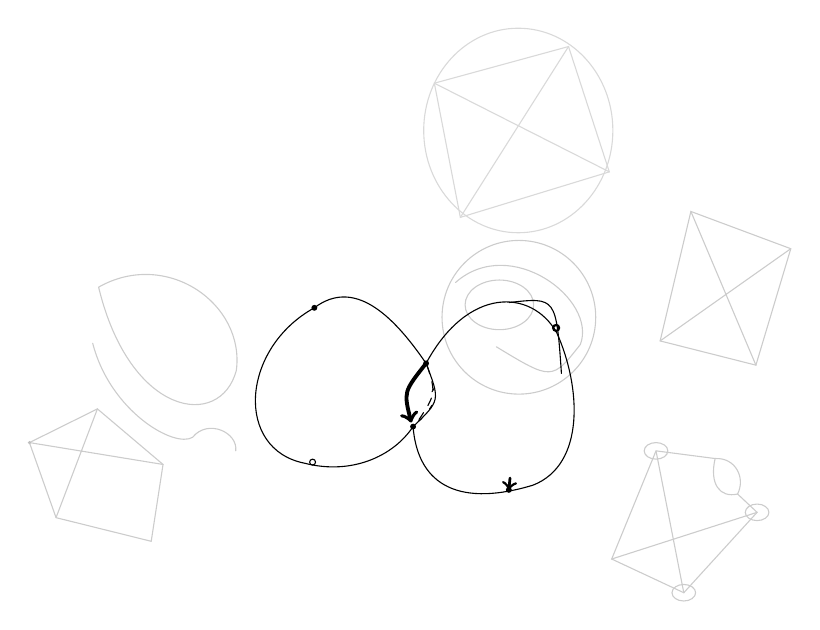
\begin{tikzpicture}[x=.0075cm,y=-.0075cm,line cap=round]
\draw[gray!30] (320,-440) ellipse (160 and 173);
\draw[gray!30] (178,-520)--(405,-582)--(474,-370)--(222,-293)--cycle;
\draw[gray!30] (178,-520)--(474,-370) (405,-582)--(222,-293);
\draw[gray!40] (-390,-175) .. controls (-275,-240) and (-142,-147) .. (-157,-34) .. controls (-184,67) and (-337,45) .. (-390,-175);
\draw[gray!40] (-400,-80) .. controls (-370,36) and (-261,98) .. (-231,79) .. controls (-205,47) and (-154,71) .. (-158,102);
\draw[gray!40] (-507,88)--(-392,31)--(-281,125)--(-301,255)--(-462,215)--cycle;
\draw[gray!40] (-507,88)--(-281,125) (-392,31)--(-462,215);
\fill[gray!50] (-507,88) circle (3);
\draw[gray!40] (321,-124) circle (130);
\draw[gray!40] (214,-183) .. controls (307,-265) and (454,-154) .. (425,-78) .. controls (377,-17) .. (283,-74);
\draw[gray!40] (288,-145) ellipse (58 and 42);
\draw[gray!40] (612,-303)--(781,-240)--(722,-43)--(560,-84)--cycle;
\draw[gray!40] (612,-303)--(722,-43) (781,-240)--(560,-84);
\draw[gray!40] (653,115) .. controls (687,113) and (705,147) .. (691,175) .. controls (661,182) and (643,158) .. (653,115);
\draw[gray!40] (553,102)--(653,115) (691,175)--(724,206)--(600,342)--(478,285)--(553,102);
\draw[gray!40] (553,102)--(600,342) (478,285)--(724,206);
\foreach \x/\y in {553/102,724/206,600/342}{\draw[gray!40] (\x,\y) ellipse (20 and 14);}
\draw (-25,-140) .. controls (-150,-71) and (-160,100) .. (-41,123) .. controls (37,143) and (108,112) .. (142,61);
\draw (-25,-140) .. controls (41,-190) and (106,-131) .. (164,-46);
\draw (164,-46) .. controls (234,-176) and (342,-173) .. (385,-98) .. controls (426,-7) and (434,125) .. (345,160) .. controls (209,201) and (149,151) .. (142,61);
\draw[->,line width=1.4pt] (164,-46) .. controls (126,2) .. (139,54);
\draw (164,-46) .. controls (188,17) .. (142,61);
\draw[dashed] (166,-42) .. controls (181,6) .. (146,58);
\draw (178,-4)--(174,2) (174,25)--(170,31) (156,48)--(151,52);
\draw (305,-149) .. controls (384,-158) .. (393,-29);
\foreach \x/\y in {-25/-140,164/-46,142/61,304/168}{\fill (\x,\y) circle (5);}
\draw[line width=.8pt] (384,-106) circle (5);
\draw (-28,121) circle (5);
\draw[->,line width=1pt] (306,148)--(304,168);
\end{tikzpicture}}% crop-candidate: scan 27
\diagram{\begin{tikzcd}[column sep=large]
\left.\begin{array}{l}
6\text{ sommets}\\(\text{dont }4\text{ ramifiés})\\
8\text{ arêtes}\\
4\ \deleted{\text{triangles}}\inserted{\text{carrés}}\;\text{--}
\end{array}\right\}
\arrow[r,Rightarrow]&
\begin{array}{l}
8\text{ sommets}\\\unsure{\text{d'ordre}|\text{dont}}4\\16\text{ arêtes}\\
8\ \deleted{\text{triangles}}\inserted{\text{carrés}}
\end{array}\arrow[d,bend right=20]\\
&\deleted{\unsure{1\times4|\text{dont }4|4\times4}\text{ d'ordre}}\ 4
\end{tikzcd}}
\figure{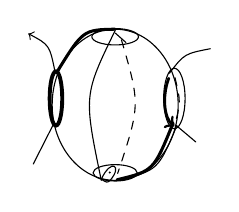
\begin{tikzpicture}[x=.8cm,y=.8cm,line cap=round]
\draw (0,0) ellipse (1 and 1.2);
\draw (0,1.08) ellipse (.37 and .13) (0,-1.08) ellipse (.35 and .13);
\draw[line width=1.4pt] (-.94,.1) ellipse (.1 and .43);
\draw (.94,.1) ellipse (.17 and .48);
\draw (.86,.5) .. controls (1.1,.81) .. (1.51,.89) (.96,-.32)--(1.28,-.59);
\draw[->] (-.95,.5)..controls (-1.04,.95)..(-1.38,1.13);
\draw (-.97,-.29)--(-1.3,-.94);
\draw (0,1.18)..controls (-.5,.15)..(-.22,-1.2);
\draw[dashed] (.1,1.03)..controls (.4,0)..(.04,-1.09);
\draw[line width=1.1pt] (-.93,.51)..controls (-.51,1.19)..(0,1.2) (.92,-.29)..controls (.61,-1.05)..(.03,-1.19);
\draw (0,1.14)--(.17,.99);
\draw (-.22,-1.18) .. controls (-.06,-.84) and (.12,-.97) .. (-.08,-1.2)
 .. controls (-.13,-1.24) .. (-.22,-1.18);
\fill (-.085,-1.075) circle (.018);
\draw[dashed] (.95,.43) .. controls (1.04,.05) .. (.95,-.31);
\draw[->,line width=1pt] (.85,.42) .. controls (.74,.12) and (.78,-.22) .. (.94,-.34);
\draw (.98,-.33) .. controls (.68,-1.04) .. (.04,-1.2);
\end{tikzpicture}}
\figure{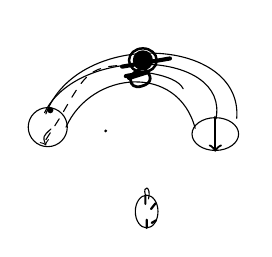
\begin{tikzpicture}[x=.8cm,y=.8cm,line cap=round]
\draw (-1.4,-.1) .. controls (-.89,1.26) and (1.73,1.13) .. (1.63,-.17);
\draw (-1.42,-.08) .. controls (-.89,1) and (1.52,.92) .. (1.3,-.18);
\draw (-1.08,-.31) .. controls (-.68,.59) and (.7,.71) .. (.97,-.33);
\draw (-1.37,-.31) circle (.31) (1.29,-.42) ellipse (.37 and .26);
\draw[->,line width=.8pt] (1.29,-.15)--(1.29,-.7);
\draw[dashed] (-1.4,-.51)--(-1.17,-.15)..controls (-.7,.67)..(.22,.68);
\fill (.14,.75) circle (.16);
\draw[line width=.9pt] (.14,.75) ellipse (.22 and .19);
\draw[line width=1pt] (.16,.62) .. controls (-.14,.58) and (-.1,.27) .. (.12,.34)
 .. controls (.31,.39) and (.28,.52) .. (.16,.62);
\draw (.24,.55) .. controls (.53,.5) and (.72,.42) .. (.78,.3);
\draw[->] (-1.32,-.34) .. controls (-1.45,-.46) .. (-1.4,-.6);
\draw[line width=1.5pt] (-.19,.65)--(.57,.78) (-.08,.47)--(.24,.57)--(-.13,.5);
\fill (-1.33,-.04) circle (.05);
\fill (-.45,-.37) circle (.025);
\draw (.2,-1.65) ellipse (.18 and .26);
\draw (.18,-1.39) .. controls (.13,-1.22) and (.28,-1.24) .. (.23,-1.45);
\draw[line width=.8pt] (.18,-1.4)--(.18,-1.53)
 (.34,-1.52)--(.27,-1.61) (.35,-1.79)--(.28,-1.83)
 (.2,-1.91)--(.2,-1.78);
\end{tikzpicture}}
\margin{Justine}% written upside down in the lower-left margin
\margin{26}

\scanpage{28}
\figure{
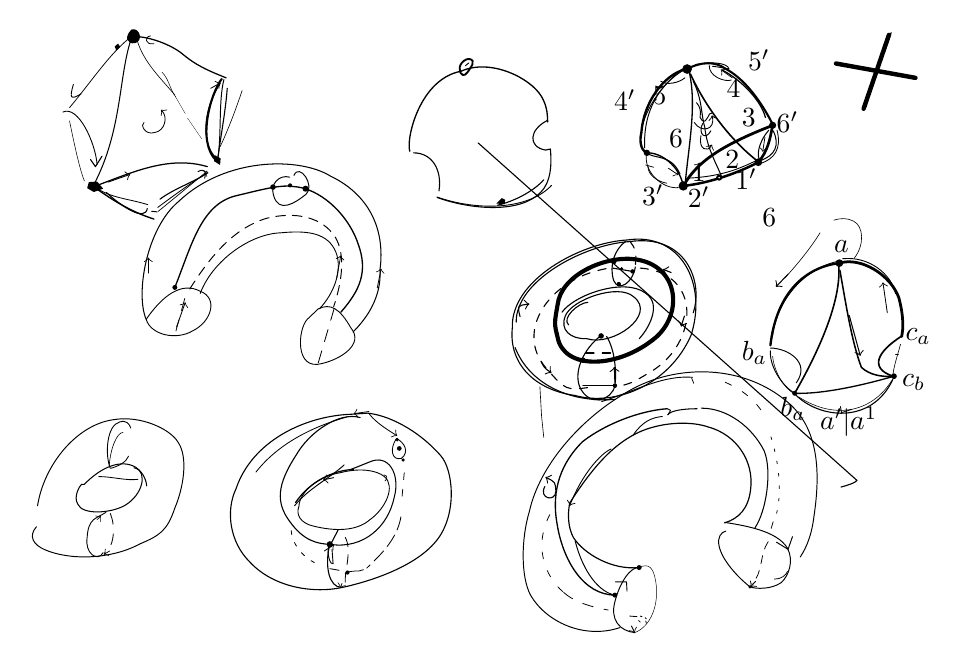
\begin{tikzpicture}[x=.007cm,y=-.007cm,line cap=round,line join=round]
\begin{scope}[shift={(83,25)},line width=.5\pgflinewidth]
\draw[line width=0.275pt] (160,38) .. controls (123,64) and (84,123) .. (46,168);
\draw[line width=0.325pt] (53,126) .. controls (46,150) and (47,155) .. (67,143);
\fill (128,57) -- (134,52) -- (138,58) -- (131,65) -- cycle;
\draw[line width=0.325pt] (34,176) .. controls (62,163) and (93,232) .. (96,271);
\draw[line width=0.2pt] (46,192) .. controls (54,231) and (64,279) .. (73,301);
\draw[line width=0.4pt] (84,262)--(93,275)--(105,256);
\draw[line width=0.375pt] (158,43) .. controls (135,110) and (142,209) .. (90,308);
\draw[line width=0.45pt] (166,39) .. controls (193,40) and (230,54) .. (250,70)
 .. controls (276,92) and (298,101) .. (330,114);
\draw[line width=0.275pt] (193,38) .. controls (181,39) and (183,55) .. (199,52);
\draw[line width=0.225pt] (168,44) .. controls (180,85) and (208,111) .. (237,145);
\draw[line width=0.175pt] (214,104) .. controls (227,117) and (228,136) .. (239,149);
\draw[line width=0.1pt] (238,148) -- (256,179);
\draw[line width=0.09pt] (260,187) -- (286,225);
\draw[line width=0.75pt] (322,116) .. controls (303,140) and (276,229) .. (312,264);
\draw[line width=0.35pt] (326,117) .. controls (316,157) and (322,213) .. (315,260);
\draw[line width=0.4pt] (319,124) .. controls (287,175) and (285,233) .. (312,260);
\draw[line width=0.4pt] (332,133) .. controls (329,175) and (319,227) .. (315,260);
\draw[line width=0.225pt] (359,137) .. controls (348,170) and (333,210) .. (319,239);
\draw[line width=0.3pt,->] (302,133) -- (320,123);
\draw[line width=0.45pt] (91,311) .. controls (165,283) and (228,255) .. (296,275);
\draw[line width=0.325pt,->] (116,303) -- (156,289);
\draw[line width=0.5pt] (92,313) .. controls (126,337) and (158,357) .. (199,370);
\draw[line width=0.3pt] (100,317) .. controls (128,333) and (157,334) .. (188,344);
\draw[line width=0.4pt] (113,322) .. controls (141,348) and (183,375) .. (187,351);
\draw[line width=0.3pt] (206,349) .. controls (234,328) and (270,302) .. (296,286);
\draw[line width=0.4pt] (210,334) .. controls (237,314) and (270,304) .. (297,286);
\draw[line width=0.25pt,->] (207,356) -- (296,283);
\draw[line width=0.35pt] (195,356) -- (205,357);
\draw[line width=0.325pt] (279,284) .. controls (290,278) and (295,283) .. (291,296);
\draw[line width=0.3pt,->] (181,195) .. controls (174,198) and (182,219) .. (201,213)
 .. controls (219,210) and (225,185) .. (212,172);
\fill (159,26) .. controls (174,23) and (180,47) .. (165,51)
 .. controls (149,54) and (145,38) .. (159,26);
\fill (81,303) -- (96,302) -- (107,315) -- (90,321) -- (78,314) -- cycle;
\fill (309,254) -- (320,260) -- (319,272) -- (308,265) -- cycle;
\end{scope}
\begin{scope}[shift={(722,26)},line width=.5\pgflinewidth]
\draw[line width=0.475pt] (24,246) .. controls (17,223) and (42,115) .. (117,101)
 .. controls (170,77) and (243,113) .. (263,147)
 .. controls (271,161) and (274,174) .. (274,193);
\draw[line width=0.4pt] (274,190) .. controls (240,207) and (238,238) .. (270,244)
 -- (279,242) .. controls (283,285) and (275,312) .. (254,327)
 .. controls (213,359) and (129,350) .. (74,330);
\draw[line width=0.4pt] (31,249) .. controls (64,249) and (83,279) .. (77,318);
\draw[line width=0.325pt] (73,329) .. controls (151,356) and (241,351) .. (281,308);
\draw[line width=0.4pt] (183,344) .. controls (213,337) and (248,319) .. (267,298);
\fill (181,341) -- (191,331) -- (197,334) -- (196,342) -- cycle;
\draw[line width=0.675pt] (115,99) .. controls (111,87) and (130,72) .. (138,82)
 .. controls (139,87) and (137,92) .. (134,95)
 .. controls (127,106) and (122,113) .. (116,104) -- cycle;
\draw[line width=0.325pt] (125,91) -- (131,86);
\end{scope}
\begin{scope}[shift={(1096,81)},line width=.5\pgflinewidth]
\draw[line width=0.85pt] (151,42) .. controls (110,52) and (74,103) .. (70,157)
 .. controls (65,178) and (72,193) .. (82,194);
\draw[line width=0.35pt] (148,43) .. controls (102,70) and (73,119) .. (76,185);
\draw[line width=0.325pt] (144,42) .. controls (113,66) and (83,104) .. (72,144);
\draw[line width=0.325pt] (105,64) .. controls (116,72) and (138,67) .. (149,58);
\draw[line width=0.75pt] (151,43) .. controls (178,28) and (204,28) .. (222,41)
 .. controls (265,64) and (295,116) .. (309,144);
\draw[line width=0.325pt] (168,34) .. controls (192,28) and (227,30) .. (229,42)
 .. controls (218,40) and (209,38) .. (199,37);
\draw[line width=0.3pt] (193,35) .. controls (192,56) and (222,66) .. (233,62);
\draw[line width=0.45pt] (217,44) .. controls (253,63) and (288,101) .. (295,130);
\draw[line width=0.95pt] (308,144) .. controls (303,171) and (299,191) .. (282,211);
\draw[line width=0.375pt] (301,153) .. controls (281,176) and (279,201) .. (285,207);
\draw[line width=0.375pt] (309,154) .. controls (322,180) and (312,199) .. (286,208);
\draw[line width=0.3pt] (316,153) .. controls (325,188) and (310,205) .. (287,213);
\draw[line width=0.9pt] (282,211) .. controls (248,229) and (195,249) .. (145,254);
\draw[line width=0.325pt] (281,207) .. controls (254,219) and (222,237) .. (152,240);
\draw[line width=0.5pt] (80,194) .. controls (106,193) and (138,218) .. (145,250);
\draw[line width=0.375pt] (80,194) .. controls (93,206) and (123,195) .. (140,232);
\draw[line width=0.275pt] (79,200) .. controls (76,228) and (107,260) .. (137,257);
\draw[line width=0.275pt] (82,218) .. controls (81,235) and (102,247) .. (116,249);
\draw[line width=0.275pt] (78,216) -- (92,220);
\draw[line width=0.475pt] (157,48) .. controls (170,107) and (157,174) .. (150,244);
\draw[line width=0.575pt] (159,51) .. controls (189,116) and (235,174) .. (282,210);
\draw[line width=1pt] (147,253) .. controls (172,206) and (229,175) .. (306,145);
\draw[line width=0.375pt] (164,64) .. controls (181,98) and (178,125) .. (185,148)
 .. controls (189,185) and (204,209) .. (215,236);
\draw[line width=0.35pt] (170,103) .. controls (184,119) and (171,130) .. (180,135)
 .. controls (190,143) and (191,118) .. (198,122);
\draw[line width=0.325pt,->] (166,139) .. controls (178,158) and (205,153) .. (198,126);
\draw[line width=0.35pt] (181,141) .. controls (172,159) and (186,173) .. (196,154);
\draw[line width=0.325pt,->] (178,163) .. controls (173,188) and (190,194) .. (198,179);
\draw[line width=0.275pt,->] (119,222) -- (137,234);
\draw[line width=0.275pt,->] (294,166) -- (290,192);
\draw[line width=0.275pt,->] (235,58) -- (214,43);
\fill (153,42) circle[radius=1.75pt];
\fill (80,194) circle[radius=1.15pt];
\fill (146,254) circle[radius=1.7pt];
\fill (211,239) circle[radius=1.1pt];
\fill[white] (211,239) circle[radius=0.325pt];
\fill (282,211) circle[radius=1.4pt];
\fill (308,144) circle[radius=1.3pt];
\node at (103,91) {$5$};
\node at (237,78) {$4$};
\node at (133,169) {$6$};
\node at (265,130) {$3$};
\node at (235,206) {$2$};
\node at (174,229) {$\unsure{1}$};
\node at (40,98) {$4'$};
\node at (283,26) {$5'$};
\node at (335,139) {$6'$};
\node at (260,242) {$1'$};
\node at (174,275) {$2'$};
\node at (91,270) {$3'$};
\node at (302,311) {$6$};
\end{scope}
\draw[line width=1.6pt] (1519,113)--(1663,139) (1615,61)--(1569,195);
\draw (1619,57)--(1606,95) (1576,174)--(1574,191);
\begin{scope}[shift={(243,275)},line width=.5\pgflinewidth]
\draw[line width=0.375pt] (25,302) .. controls (5,255) and (26,136) .. (84,88)
 .. controls (168,8) and (302,7) .. (359,42)
 .. controls (428,75) and (459,137) .. (449,212)
 .. controls (452,262) and (425,300) .. (400,325);
\draw[line width=0.475pt] (77,244) .. controls (107,169) and (124,94) .. (187,78)
 .. controls (226,69) and (267,57) .. (291,61)
 .. controls (338,63) and (390,109) .. (409,164)
 .. controls (428,215) and (413,249) .. (378,289);
\draw[line width=0.325pt] (123,255) .. controls (145,196) and (213,147) .. (269,145)
 .. controls (320,140) and (355,146) .. (369,180)
 .. controls (382,213) and (365,256) .. (339,283);
\draw[line width=0.325pt] (25,302) .. controls (55,258) and (90,233) .. (123,251)
 .. controls (156,263) and (144,306) .. (109,323)
 .. controls (80,340) and (34,331) .. (25,302);
\draw[line width=0.325pt] (337,283) .. controls (359,272) and (376,282) .. (396,317)
 .. controls (421,347) and (378,374) .. (344,382)
 .. controls (294,396) and (300,320) .. (317,302) -- (337,283);
\draw[line width=0.35pt,dash pattern=on 3.5pt off 2.5pt] (104,247) .. controls (148,177) and (189,136) .. (242,119)
 .. controls (297,105) and (345,117) .. (368,153)
 .. controls (387,185) and (380,234) .. (365,279);
\draw[line width=0.275pt,dash pattern=on 4.5pt off 3.5pt] (95,264) -- (79,323);
\draw[line width=0.3pt,dash pattern=on 4.5pt off 3.5pt] (366,282) -- (337,381);
\draw[line width=0.3pt,->] (80,316) -- (96,271);
\draw[line width=0.275pt,->] (29,218) -- (29,190);
\draw[line width=0.275pt,->] (444,245) -- (451,210);
\draw[line width=0.275pt,->] (370,229) -- (378,186);
\draw[line width=0.35pt] (285,44) .. controls (267,39) and (249,56) .. (256,77)
 .. controls (265,110) and (294,92) .. (315,75)
 .. controls (332,60) and (303,17) .. (293,41);
\fill (255,62) circle[radius=1pt];
\fill (286,59) circle[radius=0.75pt];
\fill (314,65) circle[radius=1.1pt];
\fill (77,244) circle[radius=0.9pt];
\end{scope}
\begin{scope} % A28-middle_ring
\draw (932,592) .. controls (929,506) and (1055,438) .. (1140,433) .. controls (1238,418) and (1286,513) .. (1256,606) .. controls (1216,697) and (1117,735) .. (1046,715) .. controls (973,705) and (925,658) .. (932,592);
\draw (939,582) .. controls (938,507) and (1062,441) .. (1144,436) .. controls (1247,421) and (1279,509) .. (1260,565);
\draw (937,628) .. controls (962,692) and (1033,729) .. (1119,722);
\draw[line width=1.5pt] (1014,551) .. controls (1020,495) and (1103,461) .. (1154,468) .. controls (1233,478) and (1243,564) .. (1193,609) .. controls (1125,667) and (1025,670) .. (1014,609) .. controls (1008,585) .. (1014,551);
\draw (1028,571) .. controls (1039,541) and (1125,511) .. (1152,536) .. controls (1195,569) and (1114,627) .. (1067,612) .. controls (1037,613) and (1018,596) .. (1028,571);
\draw (1022,564) .. controls (1045,532) and (1135,501) .. (1173,529) .. controls (1206,550) and (1176,598) .. (1162,612);
\draw (1034,587) .. controls (1021,575) and (1051,547) .. (1069,546);
\draw[dashed] (1102,485) .. controls (997,504) and (936,600) .. (993,665) .. controls (1029,706) .. (1074,700);
\draw[dashed] (1164,484) .. controls (1277,492) and (1270,620) .. (1183,672) .. controls (1148,693) .. (1118,700);
\draw[->] (984,653) .. controls (990,665) .. (1003,674);
\draw[->] (1244,571)--(1238,590);
\draw[->] (1220,492)--(1205,486);
\draw[->] (946,572) .. controls (941,552) .. (963,549);
\draw (1138,435) .. controls (1117,450) and (1107,480) .. (1116,507) .. controls (1125,528) and (1151,510) .. (1155,482);
\draw[dashed] (1145,435) .. controls (1157,452) .. (1155,482);
\draw (1114,484)--(1150,490);
\fill (1116,472) circle (5) (1130,485) circle (3) (1150,490) circle (4) (1125,513) circle (4);
\draw (1092,607) .. controls (1062,630) and (1043,670) .. (1054,699) .. controls (1071,737) and (1112,725) .. (1118,697);
\draw (1103,608) .. controls (1119,633) and (1121,677) .. (1118,697);
\draw[dashed] (1065,638)--(1116,638);
\draw (1060,697)--(1118,697);
\draw[->] (1118,691)--(1117,663);
\fill (1093,607) circle (5) (1060,651) circle (5) (1118,697) circle (4);
\end{scope}
\draw (870,257)--(1557,869) .. controls (1555,873) and (1540,878) .. (1528,881);
\begin{scope}[shift={(1346,385)},line width=.5\pgflinewidth]
\draw[line width=0.85pt] (179,90) .. controls (118,97) and (65,143) .. (54,239);
\draw[line width=0.3pt] (175,87) .. controls (113,101) and (66,159) .. (58,221);
\draw[line width=1pt] (179,90) .. controls (218,78) and (272,111) .. (287,153)
 .. controls (296,188) and (295,209) .. (292,223);
\draw[line width=0.325pt] (185,82) .. controls (232,77) and (273,109) .. (281,145);
\draw[line width=0.3pt,->] (266,180) -- (258,125);
\draw[line width=0.575pt] (178,96) .. controls (182,158) and (144,246) .. (98,326);
\draw[line width=0.55pt] (180,103) .. controls (191,164) and (201,231) .. (219,279)
 .. controls (233,292) and (254,297) .. (278,295);
\draw[line width=0.375pt,->] (197,185) -- (217,258);
\draw[line width=0.35pt] (54,244) .. controls (84,244) and (128,269) .. (101,307);
\draw[line width=0.35pt] (54,249) .. controls (52,276) and (74,312) .. (98,326);
\draw[line width=0.2pt] (58,259) .. controls (61,289) and (80,317) .. (96,326);
\draw[line width=0.6pt] (291,223) .. controls (249,250) and (232,280) .. (276,295);
\draw[line width=0.225pt] (290,237) .. controls (283,262) and (277,280) .. (276,295);
\draw[line width=0.275pt] (281,255) -- (286,255);
\draw[line width=0.475pt] (98,326) .. controls (155,328) and (237,307) .. (278,295);
\draw[line width=0.4pt] (98,327) .. controls (141,372) and (237,384) .. (276,301);
\draw[line width=0.2pt] (106,333) .. controls (168,373) and (236,363) .. (274,303);
\draw[line width=0.3pt] (181,350) -- (183,361) -- (202,355);
\draw[line width=0.225pt] (206,81) .. controls (225,57) and (223,23) .. (205,14)
 .. controls (194,8) and (182,8) .. (169,12);
\draw[line width=0.225pt] (144,35) .. controls (128,61) and (104,91) .. (80,117);
\draw[line width=0.375pt,->] (86,110) -- (64,133);
\fill (179,90) circle[radius=1.4pt];
\fill (98,326) circle[radius=0.9pt];
\fill (278,295) circle[radius=1.05pt];
\node at (183,60) {$a$};
\node at (25,252) {$b_a$};
\node at (95,355) {$b_a$};
\node at (322,223) {$c_a$};
\node at (314,307) {$c_b$};
\node at (196,378) {$\unsure{a'|a^1}$};
\end{scope}
\begin{scope}[shift={(35,725)},line width=.5\pgflinewidth]
\draw[line width=0.35pt] (36,190) .. controls (48,114) and (108,43) .. (173,34)
 .. controls (224,25) and (278,52) .. (291,75)
 .. controls (310,103) and (300,159) .. (285,194)
 .. controls (271,236) and (257,244) .. (222,259)
 .. controls (166,289) and (92,288) .. (50,270)
 .. controls (28,261) and (19,245) .. (34,228);
\draw[line width=0.375pt] (121,151) .. controls (152,119) and (188,105) .. (214,120)
 .. controls (236,132) and (226,170) .. (195,189)
 .. controls (169,204) and (117,207) .. (109,187)
 .. controls (101,174) and (111,156) .. (116,151) -- (121,151);
\draw[line width=0.325pt] (168,122) .. controls (158,98) and (161,44) .. (185,38)
 .. controls (197,34) and (203,42) .. (205,49);
\draw[line width=0.225pt] (166,118) .. controls (168,86) and (180,57) .. (191,57);
\draw[line width=0.3pt] (169,122) .. controls (183,118) and (197,111) .. (201,100);
\draw[line width=0.3pt] (147,137) .. controls (171,137) and (198,145) .. (218,142);
\draw[line width=0.375pt] (211,121) .. controls (225,124) and (233,142) .. (234,154);
\draw[line width=0.325pt] (160,202) .. controls (143,213) and (128,212) .. (126,247)
 .. controls (121,276) and (145,293) .. (155,275);
\draw[line width=0.3pt,dash pattern=on 4pt off 3.5pt] (168,204) .. controls (178,228) and (175,265) .. (157,278);
\draw[line width=0.225pt,->] (144,215) -- (151,209);
\draw[line width=0.25pt,->] (167,272) -- (156,278);
\end{scope}
\begin{scope}[shift={(392,715)},line width=.5\pgflinewidth]
\draw[line width=0.4pt] (248,34) .. controls (163,37) and (68,83) .. (39,169)
 .. controls (19,211) and (29,267) .. (63,301)
 .. controls (108,350) and (182,359) .. (232,348)
 .. controls (291,335) and (370,307) .. (405,260)
 .. controls (441,211) and (432,133) .. (410,109)
 .. controls (367,60) and (312,35) .. (277,32) -- (248,34);
\draw[line width=0.3pt] (75,139) .. controls (115,88) and (176,57) .. (240,39);
\draw[line width=0.4pt] (264,40) .. controls (226,29) and (172,66) .. (148,108)
 .. controls (113,162) and (111,194) .. (136,228)
 .. controls (161,263) and (185,269) .. (210,270);
\draw[line width=0.325pt] (153,201) .. controls (154,174) and (190,146) .. (228,140)
 .. controls (263,131) and (293,135) .. (308,147)
 .. controls (329,165) and (310,205) .. (282,225)
 .. controls (257,247) and (217,246) .. (180,237)
 .. controls (156,232) and (147,216) .. (153,201);
\draw[line width=0.45pt] (147,194) .. controls (172,157) and (213,136) .. (252,134);
\draw[line width=0.35pt] (145,200) .. controls (170,169) and (206,152) .. (235,126);
\draw[line width=0.375pt] (210,270) .. controls (270,279) and (315,238) .. (326,184)
 .. controls (337,143) and (316,104) .. (280,121) -- (245,135);
\draw[line width=0.25pt] (307,144) .. controls (317,146) and (311,153) .. (309,155);
\draw[line width=0.4pt] (211,269) -- (224,244);
\draw[line width=0.4pt] (209,270) .. controls (199,310) and (208,348) .. (230,348);
\draw[line width=0.3pt,dash pattern=on 3.5pt off 3pt] (237,257) .. controls (250,282) and (235,319) .. (237,341);
\draw[line width=0.275pt,->] (231,341) -- (228,349);
\draw[line width=0.325pt] (207,274) .. controls (203,289) and (211,309) .. (215,305) -- (213,279);
\draw[line width=0.3pt,->] (199,282) -- (217,270);
\draw[line width=0.3pt] (209,314) -- (226,317);
\draw[line width=0.275pt] (237,323) .. controls (249,315) and (260,321) .. (270,316);
\draw[line width=0.3pt,dash pattern=on 1.5pt off 3pt] (139,245) .. controls (140,268) and (159,292) .. (181,303);
\draw[line width=0.275pt,dash pattern=on 2.5pt off 3.5pt] (344,140) -- (339,195);
\draw[line width=0.3pt,dash pattern=on 5pt off 2pt] (338,220) .. controls (331,261) and (301,289) .. (276,313);
\draw[line width=0.3pt,->] (281,34) .. controls (294,51) and (320,66) .. (331,73);
\draw[line width=0.3pt] (330,78) .. controls (317,96) and (321,119) .. (339,114)
 .. controls (354,102) and (344,85) .. (330,78);
\fill (335,96) circle[radius=0.85pt];
\fill (331,80) circle[radius=0.7pt];
\fill (342,117) circle[radius=0.65pt];
\fill (209,270) circle[radius=1.15pt];
\draw[line width=0.275pt,->] (280,29) -- (252,33);
\draw[line width=0.325pt,->] (216,149) -- (197,153);
\fill (241,321) circle[radius=0.75pt];
\end{scope}
\begin{scope}[shift={(928,655)},line width=.5\pgflinewidth]
\draw[line width=0.35pt] (199,481) .. controls (132,503) and (64,469) .. (37,422)
 .. controls (19,388) and (20,319) .. (35,270)
 .. controls (53,188) and (126,105) .. (205,58)
 .. controls (292,2) and (416,2) .. (497,67)
 .. controls (558,113) and (564,192) .. (551,279)
 .. controls (547,312) and (538,335) .. (526,353);
\draw[line width=0.475pt] (191,422) .. controls (132,422) and (95,357) .. (85,292)
 .. controls (74,229) and (94,181) .. (131,144)
 .. controls (176,109) and (240,87) .. (285,84);
\draw[line width=0.375pt] (286,95) .. controls (291,87) and (316,84) .. (339,84);
\draw[line width=0.375pt] (347,83) .. controls (394,83) and (439,117) .. (461,161)
 .. controls (475,197) and (465,269) .. (444,300);
\draw[line width=0.425pt] (234,372) .. controls (185,377) and (135,348) .. (115,318)
 .. controls (105,300) and (104,276) .. (108,255)
 .. controls (151,188) and (189,146) .. (237,125)
 .. controls (280,107) and (330,107) .. (359,117)
 .. controls (411,131) and (443,180) .. (436,231)
 .. controls (432,265) and (415,283) .. (389,291);
\draw[line width=0.35pt] (190,422) .. controls (163,417) and (133,383) .. (118,324);
\draw[line width=0.325pt] (223,132) .. controls (240,107) and (257,100) .. (276,98);
\draw[line width=0.325pt,->] (183,157) .. controls (163,166) and (130,204) .. (108,260);
\draw[line width=0.35pt] (234,372) .. controls (219,370) and (199,398) .. (190,434)
 .. controls (181,467) and (199,487) .. (226,490);
\draw[line width=0.175pt] (234,372) .. controls (252,363) and (260,373) .. (264,397)
 .. controls (271,439) and (255,479) .. (226,490);
\draw[line width=0.325pt] (191,398)--(211,398)--(212,415);
\draw[line width=0.35pt] (389,290) .. controls (425,296) and (484,305) .. (503,337)
 .. controls (515,360) and (505,387) .. (492,399)
 .. controls (474,412) and (445,411) .. (435,407)
 .. controls (412,389) and (384,358) .. (379,333)
 .. controls (375,318) and (383,307) .. (391,306);
\draw[line width=0.35pt] (483,326)--(504,339)--(512,316);
\draw[line width=0.275pt] (479,393) .. controls (492,393) and (500,386) .. (503,379);
\draw[line width=0.275pt,dash pattern=on 3pt off 2.5pt] (468,325) .. controls (452,348) and (459,383) .. (438,402);
\draw[line width=0.325pt,->] (445,397) -- (436,407);
\draw[line width=0.275pt,dash pattern=on 2.5pt off 4.5pt] (390,36) .. controls (429,53) and (450,75) .. (466,104);
\draw[line width=0.275pt,dash pattern=on 1pt off 3.5pt] (473,135) .. controls (491,194) and (493,249) .. (479,288);
\draw[line width=0.275pt,dash pattern=on 2.5pt off 3.5pt] (477,289) -- (470,312);
\draw[line width=0.275pt,dash pattern=on 2.5pt off 4.5pt] (72,276) .. controls (43,330) and (61,387) .. (97,417);
\draw[line width=0.275pt,dash pattern=on 4pt off 4pt] (97,417) .. controls (113,432) and (142,443) .. (178,449);
\draw[line width=0.3pt] (217,460)--(230,461) (236,460)--(239,461) (245,463)--(247,465) (233,468)--(236,471) (246,469)--(247,473);
\draw[line width=0.3pt,->] (220,478) -- (226,490);
\fill (234,372) circle[radius=0.9pt];
\fill (435,407) circle[radius=0.65pt];
\draw[line width=0.3pt] (285,84)--(291,87)--(286,95);
\fill (190,422) circle[radius=0.9pt];
\draw[line width=0.225pt] (54,44) -- (57,97) -- (61,136);
\draw[line width=0.325pt] (166,71) .. controls (231,50) and (277,23) .. (331,27);
\draw[line width=0.275pt] (329,28)--(333,38);
\end{scope}
\draw[->] (991,880) .. controls (979,902) and (1010,909) .. (1011,889) .. controls (1010,872) .. (992,863);
\end{tikzpicture}
}% crop-candidate: scan 28
\begin{gather*}
4\text{ sommets}\\6\text{ arêtes}\\2\text{ \unsure{hexagones}}
\end{gather*}
\margin{27}

\cotefile{148}
\scanpage{29}
\margin{\(M_{\unsure{0|8},5}\;\unsure{-}\)}

\margin{28}

\scanpage{31}
\margin{\figure{\begin{tikzpicture}[x=1cm,y=1cm]\draw (.12,.32)--(.1,.08)..controls(.09,.01)and(.02,.01)..(0,.05);\end{tikzpicture}}}
\margin{\figure{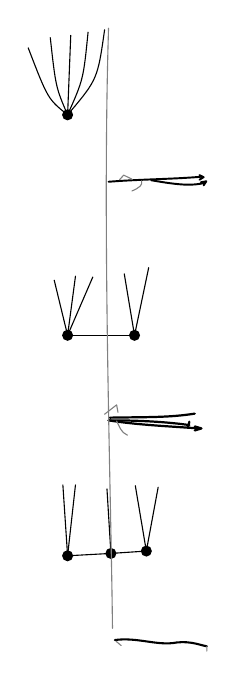
\begin{tikzpicture}[x=1cm,y=1cm,line cap=round,line join=round]
\fill (0,6.2) circle(2pt);
\draw (0,6.2)..controls(-.25,6.4)..(-.5,7.05);
\draw (0,6.2)..controls(-.15,6.55)..(-.22,7.18);
\draw (0,6.2)--(.04,7.21);
\draw (0,6.2)..controls(.2,6.65)..(.26,7.25);
\draw (0,6.2)..controls(.38,6.65)..(.47,7.28);
\draw (0,3.4)--(.85,3.4);\fill (0,3.4) circle(2pt);\fill (.85,3.4) circle(2pt);
\draw (0,3.4)--(-.17,4.1);\draw (0,3.4)--(.1,4.15);\draw (0,3.4)--(.32,4.14);
\draw (.85,3.4)--(.72,4.18);\draw (.85,3.4)--(1.03,4.26);
\draw (0,.6)--(.55,.63)--(1,.66);
\foreach \x/\y in {0/.6,.55/.63,1/.66}{\fill (\x,\y) circle(2pt);}
\draw (0,.6)--(-.06,1.5);\draw (0,.6)--(.1,1.5);\draw (.55,.63)--(.5,1.45);\draw (1,.66)--(.86,1.49);\draw (1,.66)--(1.15,1.47);
% Literal courses of the two retraced marginal arrows.
\begin{scope}[shift={(.24,5.6815)}]
\begin{scope}[x=.175cm,y=-.065cm]
\draw[line width=.7pt] (1.6,5.1)..controls (3.9,4.6) and (6.3,4.6)..(8.4,4.1);
\draw[line width=.7pt] (4.7,4.8)..controls (6.8,5.8) and (7.7,5.9)..(8.6,5.3);
\draw[gray] (2.4,4.7)--(2.7,3.8)--(3.3,4.6) (4.0,4.9)..controls (4.1,5.8) and (3.8,6.3)..(3.3,6.9);
\draw[line width=.7pt] (8.2,3.8)--(8.5,4.2)--(8.2,4.7);
\draw[line width=.7pt] (8.3,5.2)--(8.7,5.0)--(8.5,5.8);
\end{scope}
\end{scope}
\begin{scope}[shift={(.212173913,2.764637681)}]
\begin{scope}[x=.171014493cm,y=-.085507246cm]
\draw[line width=.8pt] (1.9,4.8)..controls (4.7,4.7) and (6.3,4.8)..(8.2,4.2);
\draw[line width=.8pt] (1.8,5.2)..controls (4.0,5.2) and (6.0,5.4)..(7.8,5.9);
\draw[line width=.8pt] (1.8,5.2)..controls (4.0,5.9) and (6.5,6.1)..(8.5,6.4);
\draw[gray] (1.5,4.3)--(2.4,2.9)--(2.5,4.0) (2.4,5.3)..controls (2.6,6.0) and (2.7,7.0)..(3.2,7.4);
\draw[line width=.8pt] (8.2,6.1)--(8.7,6.4)--(8.2,6.7);
\draw[line width=.8pt] (7.8,5.4)--(7.7,6.3);
\end{scope}
\end{scope}
\draw[gray] (.52,7.3)..controls(.44,4.7)and(.55,1.5)..(.57,-.32);
\begin{scope}[shift={(.328,-.0878)}]
\begin{scope}[x=.16cm,y=-.078cm]
\draw[line width=.75pt] (1.7,4.9)..controls (3.5,4.4) and (5.1,5.9)..(6.6,5.3)..controls (7.8,5.0) and (8.7,5.9)..(9.0,5.9);
\draw[gray] (1.8,5.1)--(2.2,5.8) (9.0,5.9)--(9.0,6.7);
\end{scope}
\end{scope}
\end{tikzpicture}}}


\diagram{\begin{tikzcd}[ampersand replacement=\&,column sep=9em,row sep=10em]
\begin{gathered}\mathrm{I}_{10}\ (\text{pentagonale})\\
\vcenter{\hbox{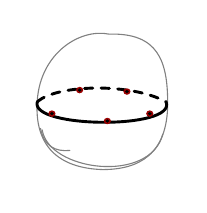
\begin{tikzpicture}[x=0.2070cm,y=-0.1870cm,line cap=round,line join=round,edge/.style={black,line width=1.05pt},rededge/.style={red!65!black,line width=.85pt},every node/.style={font=\scriptsize,inner sep=.5pt}]
\draw[gray] (1.0,5.0) .. controls (1.2,1.8) and (3.6,.1) .. (5.4,.5) .. controls (8.4,.4) and (9.0,2.3) .. (9.0,5.2) .. controls (9.0,8.7) and (7.2,9.7) .. (5.0,9.7) .. controls (2.3,9.6) and (.8,8.1) .. (1.0,5.0);
\draw[gray] (1.3,7.0) .. controls (1.7,9.8) and (7.9,10.7) .. (8.7,7.3);
\draw[gray] (1.2,6.9) .. controls (1.4,8.1) and (2.1,8.5) .. (3.0,8.4);
\draw[edge,dashed] (1.0,5.1) .. controls (2.2,3.9) and (6.8,3.8) .. (8.9,5.1);
\draw[edge] (1.0,5.1) .. controls (.5,6.9) and (9.6,7.0) .. (8.9,5.1);
\foreach \p in {(1.9,5.9),(5.3,6.4),(7.9,5.9),(3.6,4.3),(6.5,4.4)} {\fill[red!60!black] \p circle (.22);\fill[black] \p circle (.12);}
\end{tikzpicture}}}\\
\text{12 structures pentagonales sur }K\\
\{\sigma,\sigma^{-1}\}\in P_2(\mathrm{Circ}(K)\\
G\simeq\mathbb D_5\\
\widetilde G\simeq\mathbb D_5\times\{1,\sigma\}\end{gathered}\&\begin{gathered}\mathrm I_6\ (\text{bitétraédrale})\\
\vcenter{\hbox{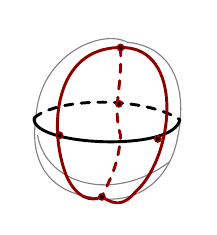
\begin{tikzpicture}[x=0.2150cm,y=-0.2230cm,line cap=round,line join=round,edge/.style={black,line width=1.05pt},rededge/.style={red!65!black,line width=.85pt},every node/.style={font=\scriptsize,inner sep=.5pt}]
\draw[gray] (1.0,5.0) .. controls (1.2,1.4) and (4.9,-.1) .. (6.4,.7) .. controls (9.6,1.0) and (10.0,4.1) .. (9.2,6.8) .. controls (8.4,9.1) and (6.4,10.0) .. (4.2,9.5) .. controls (1.8,9.2) and (.6,7.5) .. (1.0,5.0);
\draw[gray] (1.1,6.0) .. controls (1.6,8.8) and (5.6,9.9) .. (8.9,7.5);
\draw[edge,dashed] (.9,5.0) .. controls (2.4,3.8) and (7.4,3.8) .. (9.5,5.1);
\draw[edge] (.9,5.0) .. controls (.6,6.6) and (9.2,7.0) .. (9.5,5.1);
\draw[red!55!black,line width=1.05pt] (6.0,1.0) .. controls (2.1,1.0) and (1.7,5.6) .. (2.8,8.3) .. controls (3.4,9.6) and (4.3,9.8) .. (4.9,9.5);
\draw[red!55!black,line width=1.05pt] (6.0,1.0) .. controls (9.8,.9) and (9.2,7.2) .. (6.9,9.2) .. controls (6.2,10.0) and (5.7,10.0) .. (4.9,9.5);
\draw[red!55!black,line width=1.05pt,dashed] (6.0,1.0) .. controls (6.1,3.5) and (5.5,4.3) .. (6.0,6.0) .. controls (5.9,7.8) and (5.2,8.8) .. (4.9,9.5);
\foreach \p in {(6.0,1.0),(2.4,6.0),(8.2,6.2),(5.9,4.2),(4.9,9.5)} {\fill[red!60!black] \p circle (.23);\fill[black] \p circle (.12);}
\end{tikzpicture}}}\\
\text{20 structures }K=J\amalg\omega\\
\text{avec }\omega\xrightarrow{\sim}\underline\omega(J)\\
G\simeq\unsure{\mathfrak S|\mathfrak G}_J\simeq\unsure{\mathfrak S|\mathfrak G}_3\\
\widetilde G\simeq\unsure{\mathfrak S|\mathfrak G}_3\times\{1,\sigma\}\end{gathered} \arrow[r,"{3\quad f_{B,s}\quad2}","{(B\in\unsure{\mathrm{Bit\acute et}|\mathrm{Bitet}}(K),\ s\in T(B)=J)}"'] \& \begin{gathered}\mathrm I_4\ (\text{pyramidale})\\
\vcenter{\hbox{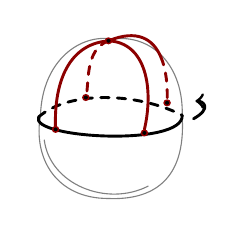
\begin{tikzpicture}[x=0.2400cm,y=-0.2250cm,line cap=round,line join=round,edge/.style={black,line width=1.05pt},rededge/.style={red!65!black,line width=.85pt},every node/.style={font=\scriptsize,inner sep=.5pt}]
\draw[gray] (.5,5.1) .. controls (.6,2.0) and (2.6,.5) .. (4.3,.8) .. controls (6.4,.5) and (8.1,2.3) .. (8.0,5.2) .. controls (8.2,8.8) and (6.4,9.9) .. (4.1,9.8) .. controls (1.3,9.8) and (.1,7.5) .. (.5,5.1);
\draw[gray] (.7,6.5) .. controls (1.0,9.0) and (4.0,10.3) .. (6.2,9.1);
\draw[edge,dashed] (.4,5.2) .. controls (2.0,3.7) and (5.6,3.8) .. (8.0,5.1);
\draw[edge] (.4,5.2) .. controls (-.1,6.4) and (8.1,6.9) .. (8.0,5.1);
\draw[red!55!black,line width=1.05pt] (4.1,.9) .. controls (1.8,1.1) and (1.2,3.6) .. (1.3,5.9);
\draw[red!55!black,line width=1.05pt] (4.1,.9) .. controls (6.1,1.0) and (6.5,3.6) .. (6.0,5.9);
\draw[red!55!black,line width=1.05pt,dashed] (4.1,.9) .. controls (2.8,1.4) and (3.1,3.4) .. (2.9,4.1);
\draw[red!55!black,line width=1.05pt] (4.1,0.9) .. controls (5.6,0.24) and (6.452,0.768) .. (6.872,1.8144);
\draw[red!55!black,line width=1.05pt,dashed] (6.872,1.8144) .. controls (7.152,2.512) and (7.24,3.44) .. (7.2,4.4);
\foreach \p in {(4.1,.9),(1.3,5.9),(6.0,6.1),(2.9,4.1),(7.2,4.4)} {\fill[red!60!black] \p circle (.20);\fill[black] \p circle (.11);}
\draw[edge,->] (8.6,5.3) .. controls (9.6,4.7) and (9.1,4.3) .. (8.7,4.3);
\end{tikzpicture}}}\\
\text{30 structures carrés orientés}\\
K=\{P\}\amalg I\\
I\ \text{structure carrée \uline{orientée}}\ (Q,\omega)=\vec Q\\
I=\coprod_{\alpha\in\delta}\alpha\qquad\delta=\text{ens. des diagonales de}\\
\omega\in\delta\wedge\bigwedge_{\alpha\in\delta}\alpha\\
G=\widetilde G=\mathbb Z/4\mathbb Z\end{gathered} \arrow[dl,bend right=10,pos=.27,"{4\quad f_{\vec Q,\omega,a}\quad2}","{(Q=\overrightarrow{\mathrm{Carr}}(K),\ a\in\Lambda(Q))}"'] \\
\begin{gathered}\mathrm{II}_2\ (\text{carré-triangle droit})\\
\vcenter{\hbox{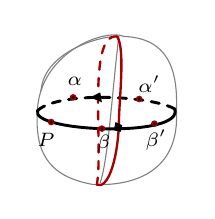
\begin{tikzpicture}[x=0.2150cm,y=-0.2090cm,line cap=round,line join=round,edge/.style={black,line width=1.05pt},rededge/.style={red!65!black,line width=.85pt},every node/.style={font=\scriptsize,inner sep=.5pt}]
\draw[gray] (.9,5.0) .. controls (1.2,1.6) and (4.9,.2) .. (6.0,.7) .. controls (8.6,.8) and (9.2,2.7) .. (9.1,5.2) .. controls (9.3,8.7) and (6.9,9.8) .. (4.2,9.7) .. controls (1.4,9.2) and (.7,7.6) .. (.9,5.0);
\draw[gray] (1.1,4.0) .. controls (1.3,1.5) and (4.9,.6) .. (5.7,.7) .. controls (5.3,4.0) and (5.1,8.0) .. (4.6,9.6);
\draw[edge,dashed] (.9,5.2) .. controls (2.2,4.0) and (7.6,4.3) .. (9.0,5.1);
\draw[edge] (.9,5.2) .. controls (.4,6.5) and (9.6,6.9) .. (9.0,5.1);
\draw[rededge] (5.6,.7) .. controls (6.1,1.5) and (5.7,4.6) .. (5.7,6.1) .. controls (5.6,8.4) and (5.0,10.0) .. (4.4,9.7);
\draw[rededge,dashed] (5.6,.7) .. controls (3.8,.5) and (4.8,7.4) .. (4.4,9.7);
\foreach \p in {(1.7,5.9),(4.7,6.3),(7.8,6.0),(3.0,4.4),(6.9,4.5)} {\fill[red!60!black] \p circle (.20);\fill[black] \p circle (.09);}
\fill (4.0,4.4)--(4.6,4.1)--(4.7,4.7)--cycle;
\fill (5.5,5.9)--(5.9,6.1)--(5.8,6.5)--(5.4,6.4)--cycle;
\node at (1.4,7.0) {$P$};\node at (4.8,7.2) {$\beta$};\node at (7.9,7.0) {$\beta'$};
\node at (3.1,3.4) {$\alpha$};\node at (7.5,3.6) {$\alpha'$};
\end{tikzpicture}}}\\
\text{2 sommets}\quad\deleted{\text{\unsure{-repères|-repère}}}\\
\text{60 structures ``pentagone}\\
\text{avec sommet'' sur }K\\
\text{i.e. }K\simeq B\amalg\omega,\ \text{avec }\omega\hookrightarrow J\\
\text{i.e. }P\in J\text{ et }\omega\simeq\omega'=B\setminus\{P\}\\
G\simeq\mathbb Z/2\mathbb Z\\
\widetilde G\simeq\mathbb Z/2\mathbb Z\times\{1,\sigma\}\end{gathered} \arrow[u,"{1\quad\gamma_{\pi,s}\quad5}","{(\pi\in\mathrm{Pent}(K),\ s\in K)}"'] \arrow[r,"{1\quad\tau_{\pi,s}=\mathrm{tw}_{1/4}\quad1}"] \& \begin{gathered}\mathrm{II}'_2=\mathrm{Tw}_{1/4}\mathrm{II}_2\\
(\text{carré-triangle gauche})\\
\text{4 sommets}\ \deleted{\text{\unsure{repères}}}\\
\vcenter{\hbox{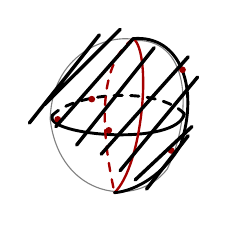
\begin{tikzpicture}[x=0.2400cm,y=-0.2330cm,line cap=round,line join=round,edge/.style={black,line width=1.05pt},rededge/.style={red!65!black,line width=.85pt},every node/.style={font=\scriptsize,inner sep=.5pt}]
% Eight explicit oblique strokes cancel this drawing; no secure alphabetic labels survive.
\draw[gray] (1.9,5.4) .. controls (2.0,1.5) and (5.4,.7) .. (6.5,1.1) .. controls (9.4,1.1) and (9.4,5.3) .. (8.1,8.1) .. controls (6.5,10.3) and (2.4,9.7) .. (1.9,5.4);
\draw[edge,dashed] (2.0,5.2) .. controls (3.2,3.9) and (7.6,3.6) .. (9.0,5.1);
\draw[edge] (2.0,5.2) .. controls (1.6,6.3) and (8.6,6.9) .. (9.0,5.1);
\draw[rededge] (6.3,1.0) .. controls (7.3,1.8) and (6.8,7.9) .. (5.3,9.4);
\draw[rededge,dashed] (6.3,1.0) .. controls (3.9,2.8) and (5.0,7.9) .. (5.3,9.4);
\draw[edge] (6.3,1.0) .. controls (8.8,.8) and (9.8,3.7) .. (8.8,6.8) .. controls (8.0,8.3) and (6.5,9.3) .. (5.3,9.4);
\foreach \p in {(2.3,5.4),(4.1,4.3),(5.0,6.0),(8.9,2.7),(8.3,7.1)} {\fill[red!60!black] \p circle (.18);}
\draw[line width=1.25pt] (.8,5.6)--(4.5,.8) (1.6,4.6)--(5.6,.5) (2.2,5.8)--(6.3,1.0) (3.3,6.8)--(7.4,1.5) (4.6,7.3)--(9.2,2.0) (5.6,8.2)--(9.7,3.1) (6.4,8.7)--(9.4,5.8) (7.0,9.2)--(9.2,6.3);
\end{tikzpicture}}}\quad\vcenter{\hbox{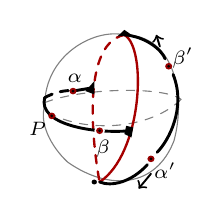
\begin{tikzpicture}[x=0.2250cm,y=-0.2100cm,line cap=round,line join=round,edge/.style={black,line width=1.05pt},rededge/.style={red!65!black,line width=.85pt},every node/.style={font=\scriptsize,inner sep=.5pt}]
\draw[gray] (1.0,4.8) .. controls (1.0,1.7) and (3.8,.1) .. (5.5,.5) .. controls (8.3,.5) and (9.0,4.1) .. (8.3,6.9) .. controls (7.3,9.7) and (4.7,10.0) .. (2.3,8.2) .. controls (1.3,7.2) and (.7,5.8) .. (1.0,4.8);
\draw[gray,dashed] (1.0,4.6) .. controls (3.1,3.7) and (7.7,3.6) .. (8.7,4.4);
\draw[gray,dashed] (1.2,5.2) .. controls (3.4,6.5) and (7.0,6.2) .. (8.7,4.4);
\draw[rededge] (5.5,.5) .. controls (6.8,1.3) and (6.5,7.7) .. (4.1,9.4);
\draw[rededge,dashed] (5.5,.5) .. controls (2.8,1.1) and (3.9,8.3) .. (4.1,9.4);
\draw[edge,dashed] (1.0,4.3) .. controls (1.5,4.0) and (2.2,3.8) .. (2.6,3.9);
\draw[edge] (1.0,4.3) .. controls (.6,5.9) and (3.7,6.5) .. (5.8,6.3);
\draw[edge] (2.6,3.9)--(3.7,3.7);
\draw[edge] (5.5,.5) .. controls (6.7,.6) and (7.6,1.4) .. (7.8,1.95);
\draw[edge] (8.25,2.9) .. controls (9.0,4.9) and (8.0,6.9) .. (7.35,7.6);
\draw[edge] (6.8,8.35) .. controls (5.9,9.4) and (4.8,9.7) .. (4.1,9.4);
\foreach \p in {(4.1,6.3)} {\fill[white] \p circle (.30);}
\foreach \p in {(1.4,5.4),(2.6,3.9),(4.1,6.3),(8.0,2.4),(7.0,8.0)} {\fill[red!60!black] \p circle (.20);\fill[black] \p circle (.09);}
\fill (3.3,3.9)--(3.8,3.3)--(3.8,4.1)--cycle;
\fill (5.6,6.0)--(6.0,6.1)--(5.9,6.7)--(5.5,6.5)--cycle;
\fill (5.1,.6)--(5.5,.2)--(5.9,.5)--cycle;\fill (3.8,9.4) circle (.15);
\draw[->,line width=.7pt] (7.5,1.2)--(7.3,.5);
\draw[->,line width=.7pt] (7.0,8.9)--(6.3,9.8);
\node at (.6,6.2) {$P$};\node at (2.7,3.1) {$\alpha$};\node at (4.3,7.4) {$\beta$};
\node at (8.8,1.9) {$\beta'$};\node at (7.8,8.7) {$\alpha'$};
\end{tikzpicture}}}\\
\text{même paramétrage que }\mathrm{II}_2\\
G\simeq\mathbb Z/2\mathbb Z,\ \widetilde G\simeq\mathbb Z/2\mathbb Z\times\{1,\sigma\}\end{gathered} \arrow[u,"{\gamma'_{\pi,s}\quad3}","{\text{comp. avec }\widetilde G;\ (\pi\in\mathrm{Pent}(K),\ s\in K)}"'] \& \begin{gathered}\mathrm{II}_1\ (\text{tétraèdre-triangle})\\
\vcenter{\hbox{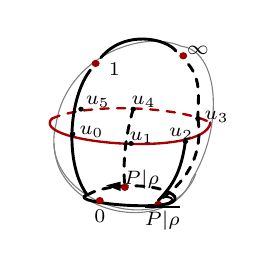
\begin{tikzpicture}[x=0.2650cm,y=-0.2420cm,line cap=round,line join=round,edge/.style={black,line width=1.05pt},rededge/.style={red!65!black,line width=.85pt},every node/.style={font=\scriptsize,inner sep=.5pt}]
\draw[gray] (.7,4.9) .. controls (1.2,1.3) and (4.9,-.1) .. (6.7,.8) .. controls (8.5,1.0) and (8.8,5.0) .. (7.2,7.8) .. controls (6.4,10.2) and (2.4,10.1) .. (1.0,7.5) .. controls (.6,6.8) and (.5,5.6) .. (.7,4.9);
\draw[gray] (.6,5.9) .. controls (.7,9.3) and (6.2,10.9) .. (7.4,7.5);
\draw[rededge,dashed] (.5,4.6) .. controls (2.3,3.7) and (6.7,4.0) .. (8.1,4.8);
\draw[rededge] (.5,4.6) .. controls (-.6,5.9) and (7.9,6.7) .. (8.1,4.8);
\draw[edge] (2.85,1.4) .. controls (4.0,-.1) and (6.0,.4) .. (6.45,1.05);
\draw[edge] (2.35,2.05) .. controls (1.3,3.5) and (1.1,7.0) .. (2.2,8.6);
\draw[edge,dashed] (7.05,1.75) .. controls (7.7,2.6) and (7.5,3.6) .. (7.5,4.6);
\draw[edge] (6.9,5.8) .. controls (6.7,7.4) and (6.3,8.1) .. (5.6,8.9);
\draw[edge,dashed] (7.5,4.6) .. controls (7.8,6.6) and (6.8,8.1) .. (5.6,8.9);
\draw[edge,dashed] (4.4,4.1) .. controls (4.0,5.6) and (3.9,7.0) .. (4.0,8.2);
\draw[edge,dashed] (2.2,8.6) .. controls (3.3,7.9) and (5.9,8.0) .. (6.4,8.7);
\draw[edge] (2.2,8.6) .. controls (1.0,9.0) and (6.8,9.6) .. (6.4,8.7);
\foreach \p in {(2.6,1.7),(6.8,1.3),(2.8,8.9),(4.0,8.2),(5.6,9.1)} {\fill[red!60!black] \p circle (.19);}
\foreach \p in {(1.5,5.4),(4.3,5.9),(6.9,5.8),(7.5,4.6),(4.4,4.1),(1.9,4.1)} {\fill \p circle (.13);}
\node at (3.5,2.0) {$1$};\node at (7.5,1.0) {$\infty$};\node at (2.8,9.7) {$0$};
\node at (4.8,7.8) {$\unsure{P|\rho}$};\node at (5.8,9.8) {$\overline{\unsure{P|\rho}}$};
\draw[line width=.7pt] (5.3,9.2)..controls (6.4,9.1) and (6.5,8.7)..(5.9,8.7);
\node at (2.4,5.3) {$u_0$};\node at (4.8,5.6) {$u_1$};\node at (6.7,5.4) {$u_2$};
\node at (8.4,4.5) {$u_3$};\node at (4.9,3.7) {$u_4$};\node at (2.7,3.7) {$u_5$};
\fill (3.1,8.1)--(3.8,7.9)--(3.8,8.4)--cycle;
\end{tikzpicture}}}\\
\text{6 sommets-repères}\\
\text{120 structures entièrement}\\
\text{épinglées,}\\
G=\deleted{\unsure{\mathbb Z_2|1}}=\{1\},\quad\widetilde G=\{1,\sigma\}\\
\left[\begin{gathered}K=J\amalg\varepsilon\quad\operatorname{card}J=3,\operatorname{card}\varepsilon=2\\\omega\in\underline\omega(J),\ r\in J\times\varepsilon\\\tau_r^0:\mathrm{II}_1(J,\varepsilon)\longrightarrow\mathrm{II}_1(u_\omega(r))\\\text{où }u_\omega=\omega\times(-1)\text{ sur }J\times\varepsilon\end{gathered}\right]\end{gathered} \arrow[ul,pos=.73,"{1\quad\gamma_r^{\unsure{0}}\quad6}","{\text{compat. avec }\widetilde G}"'] \arrow[loop right,"{\tau_r^0=\mathrm{tw}_{1/6}}"] \\
\begin{gathered}\mathrm{III}_2\ (\text{triple triangle droit})\\
\vcenter{\hbox{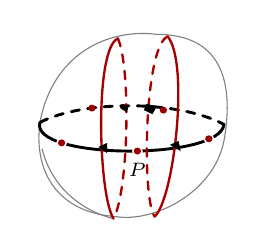
\begin{tikzpicture}[x=0.2750cm,y=-0.2600cm,line cap=round,line join=round,edge/.style={black,line width=1.05pt},rededge/.style={red!65!black,line width=.85pt},every node/.style={font=\scriptsize,inner sep=.5pt}]
\draw[gray] (.8,5.1) .. controls (1.4,1.7) and (4.0,.5) .. (6.2,.8) .. controls (9.1,.8) and (9.8,3.0) .. (9.3,6.0) .. controls (8.8,8.6) and (6.0,10.0) .. (4.3,9.7) .. controls (1.6,9.5) and (.5,7.5) .. (.8,5.1);
\draw[gray] (.9,6.4) .. controls (1.4,8.5) and (3.0,9.5) .. (4.2,9.8);
\draw[edge,dashed] (.8,5.1) .. controls (2.8,4.0) and (7.2,4.0) .. (9.3,5.2);
\draw[edge] (.8,5.1) .. controls (.3,6.9) and (9.1,7.0) .. (9.3,5.2);
\draw[rededge] (4.4,1.0) .. controls (3.3,1.5) and (3.5,8.7) .. (4.2,9.8);
\draw[rededge,dashed] (4.4,1.0) .. controls (5.0,2.4) and (4.9,8.4) .. (4.2,9.8);
\draw[rededge] (6.7,.9) .. controls (7.7,2.2) and (7.0,8.8) .. (6.1,9.7);
\draw[rededge,dashed] (6.7,.9) .. controls (5.6,1.4) and (5.5,8.9) .. (6.1,9.7);
\foreach \p in {(1.8,6.1),(5.3,6.5),(8.6,5.9)} {\fill[white] \p circle (.25);}
\foreach \p in {(1.8,6.1),(5.3,6.5),(8.6,5.9),(3.2,4.4),(6.5,4.5)} {\fill[red!60!black] \p circle (.17);}
\fill (3.5,6.3)--(3.9,6.1)--(3.9,6.6)--cycle;
\fill (6.8,6.2)--(7.2,6.0)--(7.3,6.5)--cycle;
\fill (4.6,4.2)--(4.9,4.3)--(4.8,4.6)--(4.5,4.4)--cycle;
\fill (5.7,4.2)--(6.2,4.3)--(6.0,4.7)--(5.6,4.5)--cycle;
\node at (5.3,7.4) {$P$};
\end{tikzpicture}}}\\
2+2\ \text{sommets-repère}\\
\text{60 structures ``pentagone avec}\\
\text{sommet'' sur }K,\\
G=\mathbb Z/2\mathbb Z,\widetilde G=\mathbb Z/2\mathbb Z\times\{1,\sigma\}\end{gathered} \arrow[u,start anchor=north west,"{2\quad\gamma_{\pi,\rho}\quad2}","{\begin{tikzpicture}[baseline]\draw (0,.15)..controls(-.12,.23)and(-.16,.3)..(-.14,.37);\end{tikzpicture}}"{pos=.02,description},"{(\pi\in\mathrm{Pent}(K),\rho\in\mathrm{Rep}\,\pi)}"'] \arrow[r,"{\unsure{\tau_{\pi,\omega}}}","{2\quad\tau_{\pi,\rho}=\mathrm{tw}_{1/4}\quad1}"'] \& \begin{gathered}\mathrm{III}_1\ (\text{triple triangle sem.-gauche})\\
\vcenter{\hbox{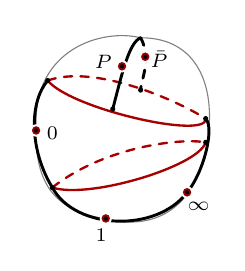
\begin{tikzpicture}[x=0.2950cm,y=-0.3020cm,line cap=round,line join=round,edge/.style={black,line width=1.05pt},rededge/.style={red!65!black,line width=.85pt},every node/.style={font=\scriptsize,inner sep=.5pt}]
\draw[gray] (1.5,5.0) .. controls (1.5,2.0) and (4.3,1.1) .. (6.0,1.5) .. controls (8.5,1.5) and (9.2,3.6) .. (8.9,5.7) .. controls (8.5,8.5) and (6.8,9.7) .. (4.4,9.1) .. controls (2.0,8.7) and (1.4,7.3) .. (1.5,5.0);
\draw[rededge,dashed] (2.0,3.3) .. controls (4.0,2.6) and (7.5,4.1) .. (8.8,4.9);
\draw[rededge] (2.0,3.3) .. controls (3.0,4.5) and (8.9,5.8) .. (8.8,4.9);
\draw[rededge,dashed] (2.2,7.8) .. controls (4.4,6.1) and (7.7,5.7) .. (8.8,5.9);
\draw[rededge] (2.2,7.8) .. controls (3.8,8.3) and (8.5,6.9) .. (8.8,5.9);
\draw[edge] (2.0,3.3) .. controls (1.2,4.2) and (1.2,6.2) .. (2.2,7.8) .. controls (3.2,9.6) and (6.7,9.7) .. (8.0,8.0) .. controls (8.7,7.2) and (9.2,5.3) .. (8.8,4.9);
\draw[edge] (4.8,4.5) .. controls (5.2,3.0) and (5.5,1.7) .. (6.0,1.5);
\draw[edge,dashed] (6.0,1.5) .. controls (6.5,2.4) and (6.0,3.3) .. (6.0,3.7);
\foreach \p in {(1.5,5.4),(4.5,9.1),(8.0,8.0),(5.2,2.7),(6.2,2.3)} {\fill[white] \p circle (.26);}
\foreach \p in {(1.5,5.4),(4.5,9.1),(8.0,8.0),(5.2,2.7),(6.2,2.3)} {\fill[red!60!black] \p circle (.18);\fill[black] \p circle (.09);}
\foreach \p in {(2.0,3.3),(4.8,4.5),(6.0,3.7),(8.8,4.9),(8.8,5.9),(2.2,7.8)} {\fill \p circle (.11);}
\node at (2.2,5.5) {$0$};\node at (4.3,9.8) {$1$};\node at (8.5,8.6) {$\infty$};
\node at (4.4,2.5) {$P$};\node at (6.8,2.4) {$\bar P$};
\end{tikzpicture}}}\quad=\quad\vcenter{\hbox{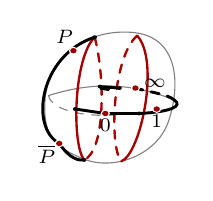
\begin{tikzpicture}[x=0.2250cm,y=-0.1900cm,line cap=round,line join=round,edge/.style={black,line width=1.05pt},rededge/.style={red!65!black,line width=.85pt},every node/.style={font=\scriptsize,inner sep=.5pt}]
\draw[gray] (1.7,5.0) .. controls (2.0,1.5) and (4.7,.3) .. (6.8,.6) .. controls (9.3,1.0) and (9.3,4.2) .. (8.7,6.4) .. controls (8.1,8.8) and (5.5,9.9) .. (3.8,9.0) .. controls (1.9,8.1) and (1.6,7.1) .. (1.7,5.0);
\draw[gray] (1.9,4.8) .. controls (4.3,3.9) and (6.5,3.9) .. (9.0,5.1);
\draw[gray,dashed] (1.9,4.8) .. controls (2.0,5.8) and (4.3,6.5) .. (6.9,5.9);
\draw[rededge] (4.5,.9) .. controls (3.3,2.3) and (3.2,8.0) .. (3.9,9.1);
\draw[rededge,dashed] (4.5,.9) .. controls (5.1,3.6) and (5.1,8.5) .. (3.9,9.1);
\draw[rededge] (6.9,.8) .. controls (8.2,2.5) and (7.1,8.7) .. (6.0,9.2);
\draw[rededge,dashed] (6.9,.8) .. controls (5.5,2.2) and (5.3,8.2) .. (6.0,9.2);
\draw[edge] (4.5,.9) .. controls (1.4,2.1) and (.8,6.9) .. (2.5,8.0) .. controls (2.9,8.7) and (3.4,9.2) .. (3.9,9.1);
\draw[edge] (3.4,5.7)--(5.1,6.0)--(7.0,6.0) .. controls (8.8,5.9) and (9.5,5.5) .. (9.0,5.1);
\draw[edge,dashed] (9.0,5.1) .. controls (8.6,4.7) and (7.7,4.6) .. (6.8,4.3);
\draw[edge] (4.8,4.2)--(5.9,4.3);
\foreach \p in {(3.3,1.8),(2.5,8.0),(5.1,6.0),(8.0,5.7),(6.8,4.3)} {\fill[white] \p circle (.26);}
\foreach \p in {(3.3,1.8),(2.5,8.0),(5.1,6.0),(8.0,5.7),(6.8,4.3)} {\fill[red!60!black] \p circle (.18);}
\foreach \p in {(4.5,.9),(3.4,5.7),(3.9,9.1),(7.0,6.0),(4.8,4.2),(5.9,4.3)} {\fill \p circle (.13);}
\fill (4.8,4.1)--(5.4,4.3)--(5.3,4.5)--(4.8,4.4)--cycle;
\node at (2.8,.9) {$P$};\node at (1.8,8.7) {$\overline P$};\node at (5.1,6.8) {$0$};\node at (8.0,6.5) {$1$};\node at (7.9,4.0) {$\infty$};
\end{tikzpicture}}}\\
\text{2+4 sommets-repère}\\
\text{120 structures épinglées}\\
G=1,\widetilde G=\{1,\sigma\}\end{gathered} \arrow[u,"{1\quad\gamma_r^1\quad2}"] \arrow[ur,"{3\qquad3}","{(r\in\mathrm{Rep}(K))}"',"{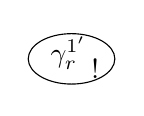
\begin{tikzpicture}[baseline=-.6ex]\draw (0,0) ellipse (.55 and .32);\node at (-.04,.07) {$\gamma_r^{1'}$};\node at (.3,-.13) {$!$};\end{tikzpicture}}"{description}] \arrow[r,"{1\quad\tau'_r\quad2}"] \& \begin{gathered}\mathrm{III}'_2\ (\text{triple triangle gauche})\\
\vcenter{\hbox{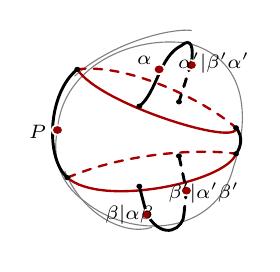
\begin{tikzpicture}[x=0.3150cm,y=-0.2750cm,line cap=round,line join=round,edge/.style={black,line width=1.05pt},rededge/.style={red!65!black,line width=.85pt},every node/.style={font=\scriptsize,inner sep=.5pt}]
\draw[gray] (1.5,5.0) .. controls (1.7,2.0) and (4.6,.6) .. (6.8,1.0) .. controls (9.3,1.8) and (9.2,4.7) .. (8.6,6.7) .. controls (7.9,9.9) and (4.5,10.1) .. (2.6,8.3) .. controls (1.5,7.4) and (1.3,6.1) .. (1.5,5.0);
\draw[gray] (2.2,2.5) .. controls (3.8,.9) and (6.1,.3) .. (6.9,.4);
\draw[gray] (1.8,6.9) .. controls (2.5,8.9) and (4.2,9.9) .. (5.3,9.5);
\draw[rededge,dashed] (2.3,2.2) .. controls (4.3,1.9) and (7.4,3.6) .. (8.7,4.9);
\draw[rededge] (2.3,2.2) .. controls (3.2,3.8) and (8.8,5.8) .. (8.7,4.9);
\draw[rededge,dashed] (1.9,7.2) .. controls (4.6,5.9) and (7.7,5.9) .. (8.7,6.1);
\draw[rededge] (1.9,7.2) .. controls (3.3,8.6) and (8.3,7.4) .. (8.7,6.1);
\draw[edge] (2.3,2.2) .. controls (1.1,3.3) and (1.0,6.3) .. (1.9,7.2);
\draw[edge] (8.7,4.9) .. controls (9.0,5.3) and (8.9,5.8) .. (8.7,6.1);
\draw[edge] (4.8,3.9) .. controls (5.5,3.3) and (5.6,1.6) .. (6.5,1.1) .. controls (6.9,.7) and (7.0,1.2) .. (6.9,1.9);
\draw[edge,dashed] (6.9,1.9)--(6.4,3.7);
\draw[edge] (4.8,7.6)--(5.1,8.9) .. controls (5.8,10.2) and (6.6,9.5) .. (6.6,8.9);
\draw[edge,dashed] (6.6,8.9)--(6.7,7.8)--(6.4,6.2);
\foreach \p in {(1.5,5.0),(5.6,2.2),(6.9,2.0),(5.1,8.9),(6.7,7.8)} {\fill[white] \p circle (.26);}
\foreach \p in {(1.5,5.0),(5.6,2.2),(6.9,2.0),(5.1,8.9),(6.7,7.8)} {\fill[red!60!black] \p circle (.18);}
\foreach \p in {(2.3,2.2),(4.8,3.9),(6.4,3.7),(8.7,4.9),(8.7,6.1),(6.4,6.2),(4.8,7.6),(1.9,7.2)} {\fill \p circle (.12);}
\node at (.7,5.1) {$P$};\node at (5.0,1.8) {$\alpha$};
\node at (7.8,1.9) {$\unsure{\alpha'|\deleted{\beta'}\inserted{\alpha'}}$};
\node at (4.4,8.9) {$\unsure{\beta|\deleted{\alpha}\inserted{\beta}}$};
\node at (7.4,7.9) {$\unsure{\beta'|\deleted{\alpha'}\inserted{\beta'}}$};
\end{tikzpicture}}}\quad\simeq\quad\vcenter{\hbox{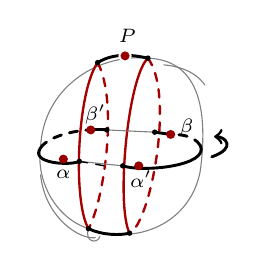
\begin{tikzpicture}[x=0.2900cm,y=-0.2850cm,line cap=round,line join=round,edge/.style={black,line width=1.05pt},rededge/.style={red!65!black,line width=.85pt},every node/.style={font=\scriptsize,inner sep=.5pt}]
\draw[gray] (.7,5.4) .. controls (.8,2.8) and (3.1,1.2) .. (5.4,1.4) .. controls (7.8,1.5) and (8.0,4.0) .. (7.7,6.4) .. controls (7.3,8.7) and (5.0,9.8) .. (2.8,9.0) .. controls (1.3,8.5) and (.5,6.8) .. (.7,5.4);
\draw[gray] (.7,6.6) .. controls (.9,8.5) and (2.4,9.5) .. (3.1,9.4);
\draw[gray] (6.1,1.7) .. controls (7.2,1.8) and (7.7,2.3) .. (7.9,2.6);
\draw[rededge] (3.2,1.6) .. controls (2.3,2.9) and (2.1,7.8) .. (2.8,9.0);
\draw[rededge,dashed] (3.2,1.6) .. controls (4.1,3.3) and (3.5,7.7) .. (2.8,9.0);
\draw[rededge] (5.4,1.4) .. controls (4.5,2.3) and (4.0,8.0) .. (4.6,9.2);
\draw[rededge,dashed] (5.4,1.4) .. controls (6.6,3.0) and (5.5,8.8) .. (4.6,9.2);
\draw[edge] (3.2,1.6) .. controls (4.0,1.1) and (4.9,1.3) .. (5.4,1.4);
\draw[edge] (2.8,9.0) .. controls (3.4,9.3) and (4.2,9.3) .. (4.6,9.2);
\draw[gray] (2.4,6.0)--(4.3,6.2);
\draw[gray] (3.6,4.6)--(5.7,4.7);
\draw[edge,dashed] (.7,5.4) .. controls (1.1,4.8) and (2.6,4.5) .. (3.6,4.6);
\draw[edge] (.7,5.4) .. controls (.2,6.1) and (2.0,6.2) .. (2.4,6.0);
\draw[line width=.5pt,dashed] (2.4,6.0)--(3.5,6.2);
\draw[edge] (4.3,6.2) .. controls (5.2,6.5) and (8.1,6.2) .. (7.7,5.3);
\draw[edge,dashed] (7.7,5.3) .. controls (7.4,4.8) and (6.7,4.8) .. (6.4,4.8);
\draw[edge] (6.4,4.8)--(5.7,4.7);
\draw[edge] (2.9,4.6)--(3.6,4.6);
\draw[gray] (2.8,9.0)..controls(2.6,9.6)and(3.2,9.7)..(3.3,9.35);
\foreach \p in {(4.4,1.3)} {\fill[white] \p circle (.29);}
\foreach \p in {(4.4,1.3),(1.7,5.9),(5.0,6.2),(2.9,4.6),(6.4,4.8)} {\fill[red!60!black] \p circle (.20);}
\foreach \p in {(3.2,1.6),(5.4,1.4),(2.8,9.0),(4.6,9.2),(2.4,6.0),(4.3,6.2),(3.6,4.6),(5.7,4.7)} {\fill \p circle (.12);}
\node at (4.5,.4) {$P$};\node at (1.7,6.6) {$\alpha$};\node at (5.1,6.8) {$\alpha'$};\node at (3.1,3.9) {$\beta'$};\node at (7.1,4.5) {$\beta$};
\draw[edge,->] (8.2,5.8) .. controls (9.3,5.4) and (8.8,4.9) .. (8.3,4.9);
\end{tikzpicture}}}\\
\text{4+4 sommets-repère}\\
\text{60 structures de carré orienté à}\\
\text{\unsure{codiagonales|codiagonale}, }K=\{P\}\amalg I,\\
I\ \text{muni d’une \inserted{str.} \unsure{carré|carrée} en \unsure{codiagonales|codiagonale} }\delta=\{\{\alpha,\beta\},\{\alpha',\beta'\}\}\\
\text{i.e. d’un repère de }\unsure{\mathfrak X|\mathbb J}\unsure{(}I)\\
G=\mathbb Z/2\mathbb Z\unsure{\deleted{*}},\quad\widetilde G\simeq\mathbb Z/2\mathbb Z\times\mathbb Z/2\mathbb Z\simeq\mathbb Z/2\mathbb Z\times\{1,\sigma\}\end{gathered} \arrow[uu,bend right=70,"{1\quad\gamma_r^{2'}\quad2}"] \arrow[ull,bend left=65,"{2\quad\gamma_r^2\quad2}"']
\end{tikzcd}}
% crop-candidate: scan 31

\diagram{\[\begin{array}{lll}
\uline{\text{niveau }2}&\mathrm I_{10},\mathrm I_6,\mathrm I_4&12+20+30=62\\
\uline{\text{niveau }}1&\mathrm{II}_2,\mathrm{II}'_2,\mathrm{II}_1&60+60+120=240\\
\uline{\text{niveau }}0&\mathrm{III}_2,\mathrm{III}_4,\mathrm{III}'_2&60+120+60=240\\
&&\overline{542}
\end{array}\]}

(l’indice ``i'' indique l’ordre du \(G=\operatorname{Aut}^{+}\unsure{\}|)}\), donc le nb de structures \deleted{est} \(120/i\))

\uline{NB} Sauf \(\mathrm I_4\), toutes ces structures sont ``réelles''.

\[\begin{array}{ll}
\pi\in\mathrm{Pent}(K),&B\in\mathrm{Bit\acute et}(K)\\
s\in K,&\vec Q\in\overrightarrow{\mathrm{Carr}}(K)\\
\rho\in\mathrm{Rep}(\pi);&r\in\mathrm{Rep}(K)
\end{array}\]
(\uline{NB} \(\{(\pi,\rho)\}\unsure{\simeq}\mathrm{Rep}(K)\)).
\margin{30}

\scanpage{32}
\figure{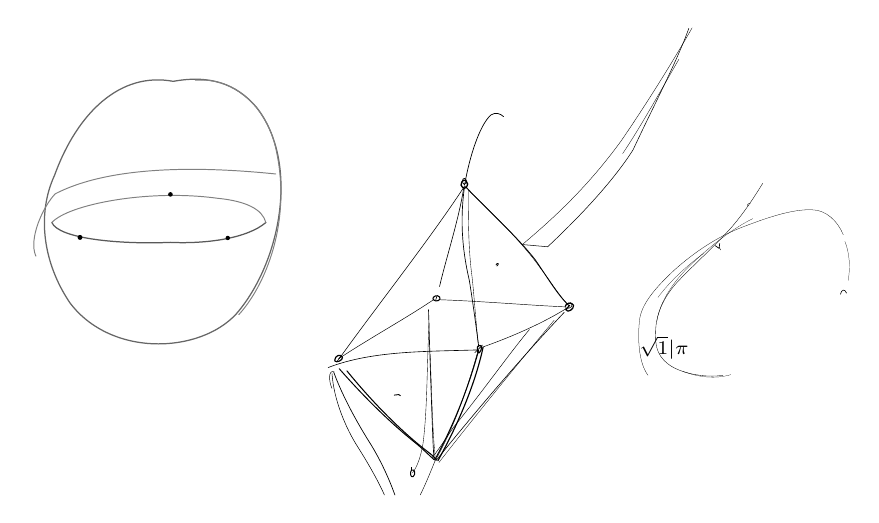
\begin{tikzpicture}[x=.007cm,y=-.007cm,line cap=round,line join=round]
\draw[black!60,line width=.45pt] (1550,418)
 .. controls (1454,400) and (1376,475) .. (1335,588)
 .. controls (1302,659) and (1314,748) .. (1363,820)
 .. controls (1438,919) and (1599,912) .. (1665,839)
 .. controls (1745,746) and (1780,566) .. (1701,465)
 .. controls (1664,422) and (1616,406) .. (1550,418);
\draw[black!50,line width=.35pt] (1590,416)
 .. controls (1664,410) and (1718,467) .. (1735,535)
 .. controls (1768,673) and (1715,791) .. (1669,841);
\draw[black!65,line width=.45pt] (1330,674)
 .. controls (1342,703) and (1450,714) .. (1545,710)
 .. controls (1610,713) and (1684,703) .. (1718,674);
\draw[black!50,line width=.35pt] (1330,674)
 .. controls (1360,641) and (1505,613) .. (1630,630)
 .. controls (1682,635) and (1712,650) .. (1718,674);
\draw[black!50,line width=.35pt] (1301,735)
 .. controls (1287,704) and (1314,645) .. (1336,622)
 .. controls (1425,576) and (1571,569) .. (1736,586);
\fill (1381,701) circle (4.5);
\fill (1649,702) circle (4);
\fill (1545,623) circle (4.2);
\begin{scope}[shift={(1822,324)},line width=0.58333333\pgflinewidth]
\draw[line width=0.256667pt] (257,279) .. controls (265,233) and (283,174) .. (304,155)
 .. controls (313,149) and (322,153) .. (327,158);
\draw[line width=0.128333pt] (669,-3) .. controls (629,67) and (580,144) .. (541,201)
 .. controls (483,281) and (423,338) .. (361,390);
\draw[line width=0.186667pt] (663,-2) .. controls (642,57) and (596,145) .. (562,218)
 .. controls (528,272) and (468,337) .. (407,394) -- (362,390);
\draw[line width=0.116667pt] (645,54) .. controls (606,122) and (569,187) .. (543,225);
\draw[line width=0.198333pt] (257,283) .. controls (196,377) and (91,510) .. (29,597);
\draw[line width=0.175pt] (28,597) .. controls (84,560) and (148,525) .. (200,490);
\draw[line width=0.221667pt] (9,613) .. controls (89,582) and (188,584) .. (281,581);
\draw[line width=0.175pt] (283,578) .. controls (338,559) and (398,533) .. (444,504);
\draw[line width=0.163333pt] (211,490) .. controls (294,493) and (371,500) .. (440,503);
\draw[line width=0.320833pt] (258,285) .. controls (301,330) and (350,374) .. (384,417)
 .. controls (407,450) and (425,481) .. (445,500);
\draw[line width=0.116667pt] (263,291) .. controls (319,344) and (363,390) .. (392,430)
 .. controls (414,459) and (430,486) .. (446,501);
\draw[line width=0.2275pt] (255,286) .. controls (246,345) and (223,414) .. (211,466);
\draw[line width=0.245pt] (256,287) .. controls (247,353) and (254,408) .. (265,455)
 .. controls (271,492) and (278,543) .. (282,575);
\draw[line width=0.134167pt] (263,291) .. controls (263,356) and (264,405) .. (270,449)
 .. controls (274,486) and (277,532) .. (281,568);
\draw[line width=0.233333pt] (191,508) .. controls (193,578) and (196,669) .. (199,746)
 .. controls (200,760) and (200,775) .. (202,781);
\draw[line width=0.134167pt] (192,532) .. controls (188,608) and (189,690) .. (181,751)
 .. controls (177,775) and (170,794) .. (162,804);
\draw[line width=0.116667pt] (194,589) .. controls (197,664) and (198,723) .. (203,774);
\draw[line width=0.35pt] (29,615) .. controls (72,664) and (121,713) .. (169,751)
 .. controls (181,761) and (192,772) .. (201,780);
\draw[line width=0.379167pt] (43,619) .. controls (91,678) and (144,731) .. (190,766)
 .. controls (198,772) and (202,776) .. (206,781);
\draw[line width=0.250833pt] (19,621) .. controls (33,660) and (58,707) .. (83,747)
 .. controls (104,780) and (120,816) .. (130,844);
\draw[line width=0.1925pt] (16,624) .. controls (19,670) and (40,722) .. (64,759)
 .. controls (88,797) and (103,826) .. (111,844);
\draw[line width=0.169167pt] (20,621) .. controls (9,616) and (10,638) .. (16,651);
\draw[line width=0.361667pt] (282,581) .. controls (264,648) and (236,719) .. (203,779);
\draw[line width=0.408333pt] (290,576) .. controls (277,637) and (248,710) .. (208,782);
\draw[line width=0.151667pt] (279,589) .. controls (257,666) and (234,727) .. (202,784)
 .. controls (193,807) and (183,830) .. (176,844);
\draw[line width=0.215833pt] (437,513) .. controls (365,589) and (280,688) .. (206,780);
\draw[line width=0.116667pt] (419,527) .. controls (357,601) and (277,699) .. (210,785);
\draw[line width=0.163333pt] (374,544) .. controls (338,587) and (288,658) .. (235,723)
 .. controls (221,744) and (207,765) .. (197,777);
\draw[line width=0.478333pt] (261,278) .. controls (259,269) and (250,273) .. (250,282)
 .. controls (252,289) and (261,291) .. (262,280) -- (259,276);
\draw[line width=0.245pt] (256,275) ellipse (3.5 and 5.2);
\fill (256,281) circle (1.3);
\draw[line width=0.4375pt] (21,599) .. controls (22,591) and (31,588) .. (35,594)
 .. controls (36,600) and (24,605) .. (21,601);
\draw[line width=0.1925pt] (25,602) -- (32,592);
\draw[line width=0.396667pt] (199,489) .. controls (198,484) and (207,480) .. (211,485)
 .. controls (216,491) and (203,495) .. (200,490);
\draw[line width=0.233333pt] (206,484) -- (204,491);
\draw[line width=0.455pt] (439,502) .. controls (440,495) and (451,494) .. (454,500)
 .. controls (455,507) and (443,515) .. (440,508) -- (447,500);
\draw[line width=0.21pt] (439,505) .. controls (448,508) and (456,500) .. (448,495);
\draw[line width=0.42pt] (280,575) .. controls (286,570) and (289,574) .. (286,582)
 .. controls (282,590) and (278,588) .. (280,575);
\draw[line width=0.175pt] (275,586) -- (289,572);
\draw[line width=0.35pt] (160,799) .. controls (166,796) and (169,806) .. (163,811)
 .. controls (158,813) and (157,803) .. (160,799);
\draw[line width=0.233333pt] (160,800) -- (160,794);
\draw[line width=0.320833pt] (129,663) -- (137,662) -- (140,664);
\draw[line width=0.2625pt] (313,427) .. controls (317,421) and (320,425) .. (315,429);
\end{scope}
\begin{scope}[shift={(2384,605)},line width=0.35000000\pgflinewidth]
\draw[line width=0.098pt] (27,346) .. controls (9,322) and (8,275) .. (12,243)
 .. controls (17,213) and (45,183) .. (75,155)
 .. controls (112,122) and (154,94) .. (199,77)
 .. controls (241,61) and (289,44) .. (325,46)
 .. controls (349,46) and (371,66) .. (381,91);
\draw[line width=0.077pt] (384,103) .. controls (393,126) and (394,151) .. (390,174);
\draw[line width=0.126pt] (235,-2) .. controls (219,24) and (195,61) .. (169,88)
 .. controls (143,116) and (112,144) .. (83,174)
 .. controls (54,204) and (39,240) .. (41,274)
 .. controls (39,303) and (53,324) .. (82,336)
 .. controls (106,346) and (139,350) .. (163,346);
\draw[line width=0.063pt] (217,62) .. controls (176,82) and (130,120) .. (98,152)
 .. controls (68,183) and (48,216) .. (43,248);
\draw[line width=0.063pt] (45,205) .. controls (66,176) and (99,146) .. (128,125);
\draw[line width=0.0665pt] (90,339) .. controls (121,350) and (148,353) .. (177,345);
\draw[line width=0.0875pt] (210,39) .. controls (204,39) and (208,33) .. (213,34);
\draw[line width=0.245pt] (149,111) -- (156,116) -- (157,107);
\draw[line width=0.1225pt] (156,114) -- (159,119);
\node[inner sep=0,font=\scriptsize] at (56,296) {$\unsure{\sqrt{1}|\pi}$};
\draw[line width=0.217pt] (376,199) .. controls (378,190) and (384,189) .. (387,197);
\end{scope}
\end{tikzpicture}}

% The mechanical listing is upside down relative to the pencil sketches.
\figure{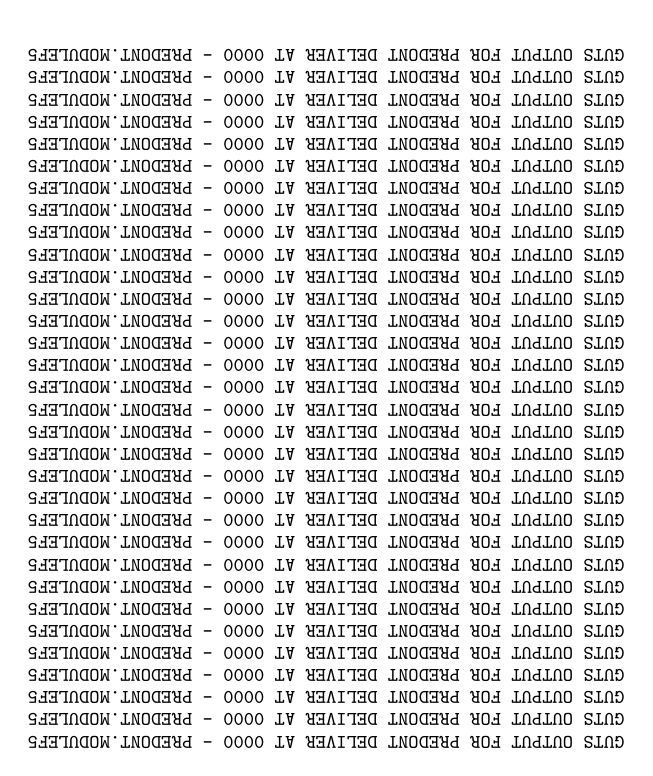
\begin{tikzpicture}
\node[rotate=180,align=left,font=\scriptsize,inner sep=0pt] {
\texttt{GUTS OUTPUT FOR PREDONT DELIVER AT 0000 - PREDONT.MODULEF5}\\
\texttt{GUTS OUTPUT FOR PREDONT DELIVER AT 0000 - PREDONT.MODULEF5}\\
\texttt{GUTS OUTPUT FOR PREDONT DELIVER AT 0000 - PREDONT.MODULEF5}\\
\texttt{GUTS OUTPUT FOR PREDONT DELIVER AT 0000 - PREDONT.MODULEF5}\\
\texttt{GUTS OUTPUT FOR PREDONT DELIVER AT 0000 - PREDONT.MODULEF5}\\
\texttt{GUTS OUTPUT FOR PREDONT DELIVER AT 0000 - PREDONT.MODULEF5}\\
\texttt{GUTS OUTPUT FOR PREDONT DELIVER AT 0000 - PREDONT.MODULEF5}\\
\texttt{GUTS OUTPUT FOR PREDONT DELIVER AT 0000 - PREDONT.MODULEF5}\\
\texttt{GUTS OUTPUT FOR PREDONT DELIVER AT 0000 - PREDONT.MODULEF5}\\
\texttt{GUTS OUTPUT FOR PREDONT DELIVER AT 0000 - PREDONT.MODULEF5}\\
\texttt{GUTS OUTPUT FOR PREDONT DELIVER AT 0000 - PREDONT.MODULEF5}\\
\texttt{GUTS OUTPUT FOR PREDONT DELIVER AT 0000 - PREDONT.MODULEF5}\\
\texttt{GUTS OUTPUT FOR PREDONT DELIVER AT 0000 - PREDONT.MODULEF5}\\
\texttt{GUTS OUTPUT FOR PREDONT DELIVER AT 0000 - PREDONT.MODULEF5}\\
\texttt{GUTS OUTPUT FOR PREDONT DELIVER AT 0000 - PREDONT.MODULEF5}\\
\texttt{GUTS OUTPUT FOR PREDONT DELIVER AT 0000 - PREDONT.MODULEF5}\\
\texttt{GUTS OUTPUT FOR PREDONT DELIVER AT 0000 - PREDONT.MODULEF5}\\
\texttt{GUTS OUTPUT FOR PREDONT DELIVER AT 0000 - PREDONT.MODULEF5}\\
\texttt{GUTS OUTPUT FOR PREDONT DELIVER AT 0000 - PREDONT.MODULEF5}\\
\texttt{GUTS OUTPUT FOR PREDONT DELIVER AT 0000 - PREDONT.MODULEF5}\\
\texttt{GUTS OUTPUT FOR PREDONT DELIVER AT 0000 - PREDONT.MODULEF5}\\
\texttt{GUTS OUTPUT FOR PREDONT DELIVER AT 0000 - PREDONT.MODULEF5}\\
\texttt{GUTS OUTPUT FOR PREDONT DELIVER AT 0000 - PREDONT.MODULEF5}\\
\texttt{GUTS OUTPUT FOR PREDONT DELIVER AT 0000 - PREDONT.MODULEF5}\\
\texttt{GUTS OUTPUT FOR PREDONT DELIVER AT 0000 - PREDONT.MODULEF5}\\
\texttt{GUTS OUTPUT FOR PREDONT DELIVER AT 0000 - PREDONT.MODULEF5}\\
\texttt{GUTS OUTPUT FOR PREDONT DELIVER AT 0000 - PREDONT.MODULEF5}\\
\texttt{GUTS OUTPUT FOR PREDONT DELIVER AT 0000 - PREDONT.MODULEF5}\\
\texttt{GUTS OUTPUT FOR PREDONT DELIVER AT 0000 - PREDONT.MODULEF5}\\
\texttt{GUTS OUTPUT FOR PREDONT DELIVER AT 0000 - PREDONT.MODULEF5}\\
\texttt{GUTS OUTPUT FOR PREDONT DELIVER AT 0000 - PREDONT.MODULEF5}\\
\texttt{GUTS OUTPUT FOR PREDONT DELIVER AT 0000 - PREDONT.MODULEF5}\\
};
\end{tikzpicture}}
\margin{31}

\scanpage{33}

\diagram{\[
\begin{array}{rll}
180 &
\left\{\begin{array}{l}
60=3\times20=2\times30\\
120=4\times30=2\times60
\end{array}\right. &
\begin{array}{l}f_{B,s}\\f_{\vec Q,a}\end{array}\\[1em]
420 &
\left\{\begin{array}{l}
60=1\times60=4\times60\\
\inserted{120=1\times120=1\times\unsure{220|120}}\\
60=1\times60=5\times12\\
60=1\times60=3\times20\\
120=1\times120=6\times20
\end{array}\right. &
\begin{array}{l}
\tau_{\pi,s}\\
\inserted{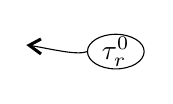
\begin{tikzpicture}[baseline=(z.base),x=1cm,y=1cm]
\node (z) at (.7,0) {$\tau_r^0$};
\draw (.7,0) ellipse (.36 and .22);
\draw (-.4,.08)..controls(-.1,.03)and(.2,-.05)..(.34,0);
\draw[line width=1.1pt](-.25,.16)--(-.4,.08)--(-.25,-.03);
\end{tikzpicture}}\\
\gamma_{\pi,s}\\
\gamma'_{\pi,s}\\
\gamma_r^0
\end{array}\\[1em]
\begin{array}{r}\inserted{1020}\\\deleted{\unsure{900|780}}\end{array} &
\left\{\begin{array}{l}
120=2\times60=1\times120\\
120=\unsure{2\times60|\deleted{1\times120}\inserted{2\times60}}=2\times60\\
120=\unsure{1\times120|\deleted{2\times60}\inserted{1\times120}}=2\times60\\
120=1\times120=2\times60\\
\inserted{3\times}120=\deleted{\unsure{1\times120=2\times60|2\times60=2\times60}}\inserted{3\times40=3\times40}\\
120=2\times60=2\times60\\
60=1\times60=2\times30
\end{array}\right. &
\begin{array}{l}
\tau_{\pi,\rho}\\
\gamma_{\pi,\rho}\\
\left.\begin{array}{l}
\unsure{\tau'|\tau}_{\deleted{\unsure{\pi,\rho}}\inserted{r}}\\
\gamma_r^1\\
\gamma_r^{1'}\\
\gamma_r^2\\
\gamma_r^{2'}
\end{array}\right\}
\end{array}
\end{array}
\]}

\[
\begin{array}{r}
\overline{\overline{\deleted{\unsure{1580|1380}}}}\\
\inserted{1620}
\end{array}
=5\times60+\deleted{\unsure{9|12}}\inserted{11}\times120
\]

\[
\begin{array}{l}
\tau=\text{``twist''}\\
\gamma=\text{``gommage''}
\end{array}
\]

Programme de travail :

1) déterminer \unsure{un|les} syst. fondamental de
relations entre les \(1620\) flèches
du diagramme, se partageant
\deleted{entre} \(14\) \deleted{\unsure{paquets} de}\inserted{orbites} sous \(\unsure{\mathfrak G_K|\mathfrak S_K}\) (\unsure{aux|avec} \(542\)
sommets, se partageant \deleted{entre} \(9\) orbites)

\margin{\figure{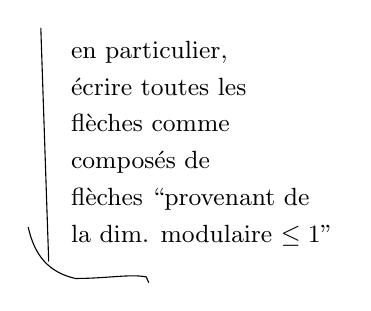
\begin{tikzpicture}[x=.01cm,y=-.01cm,line cap=round,line join=round]
\node[anchor=north west,align=left,font=\small] at (42,15) {
en particulier,\\[.08cm]
écrire toutes les\\[.08cm]
flèches comme\\[.08cm]
composés de\\[.08cm]
flèches ``provenant de\\[.08cm]
la dim. modulaire \(\leq1\)''
};
\draw[line width=.4pt] (16,11)--(26,307);
\draw[line width=.4pt] (0,264)..controls(8,299)and(25,321)..(60,329)..controls(100,329)and(130,323)..(150,327)--(153,334);
\end{tikzpicture}}}

\deleted{2) \unsure{Éli.|Réduire}}

2) Reprendre la question, en éliminant
les sommets \unsure{du|de} niveau \(0\) (sauf
peut-être ceux de type \(\mathrm I_{\unsure{20|10}}\) ?),
\deleted{et \(\mathrm{II}_1\) \deleted{\unsure{ceux}} (\unsure{ceux|qui} de type \(\mathrm{II}_1\) (qui \unsure{reviennent|revient}
à ceux de type \(\mathrm{III}_1\).) --- mais - Attention
au twist \inserted{\(\mathrm{tw}_{1/6}\)} \unsure{relativement|relationnel|relèvement} : \(\mathrm{II}_1\) (qui donne
\unsure{un Autom.} de \(=\) type))}

3) Eliminer de plus les pièces
\deleted{``\unsure{gauches}} \inserted{``tétraédrales''} \(\mathrm{II}_1\) --- et toutes
les pièces qui ne semblent pas
simplifier la présentation des relations.

\figure{\begin{tikzpicture}[x=.006cm,y=-.006cm,line cap=round,line join=round,
ink/.style={draw=black,line width=.6pt},
fine/.style={draw=black,line width=.35pt},
pencil/.style={draw=gray,line width=.35pt},
cut/.style={draw=green!40!black,line width=.8pt,dash pattern=on 1.2pt off 1.3pt},
cutsolid/.style={draw=green!40!black,line width=.8pt}]
% S033 pants
\draw[ink] (2343,133)..controls(2347,181)and(2338,216)..(2317,242);
\draw[ink] (2406,130)..controls(2413,177)and(2430,182)..(2480,180);
\draw[ink] (2482,232)..controls(2428,229)and(2400,244)..(2366,270);
\draw[ink] (2342,129)..controls(2336,117)and(2360,109)..(2380,113)..controls(2402,112)and(2415,118)..(2407,128)..controls(2390,141)and(2354,143)..cycle;
\draw[ink] (2317,242)..controls(2332,231)and(2344,237)..(2356,245)..controls(2370,254)and(2376,266)..(2366,273)..controls(2348,274)and(2328,261)..cycle;
\draw[ink] (2483,180)..controls(2497,176)and(2508,195)..(2504,215)..controls(2502,240)and(2483,243)..(2478,224)..controls(2472,208)and(2476,190)..cycle;
\draw[ink] (2341,239)..controls(2370,210)and(2391,174)..(2411,164)--(2418,170);
\draw[fine,dash pattern=on 1.1pt off 1.3pt] (2346,271)..controls(2382,244)and(2409,209)..(2425,178);
\draw[pencil] (2355,141)..controls(2350,178)and(2351,219)..(2342,240);
\draw[pencil] (2388,142)..controls(2420,172)and(2451,198)..(2481,202);
\draw[pencil] (2285,206)--(2308,145);
\draw[pencil] (2483,275)--(2517,244);
% S033 four_top
\draw[ink] (2649,129)..controls(2675,142)and(2702,145)..(2720,147);
\draw[ink] (2737,145)..controls(2752,142)and(2765,136)..(2766,131);
\draw[ink] (2798,152)..controls(2794,184)and(2794,213)..(2811,236);
\draw[ink] (2790,270)..controls(2768,233)and(2727,234)..(2684,283);
\draw[ink] (2634,260)..controls(2643,244)and(2649,234)..(2648,225);
\draw[ink] (2648,207)..controls(2652,191)and(2641,162)..(2632,153);
\draw[ink] (2616,149)..controls(2611,140)and(2636,118)..(2646,121)..controls(2660,124)and(2650,145)..(2624,155)..controls(2617,156)and(2615,154)..cycle;
\draw[ink] (2764,131)..controls(2773,115)and(2809,138)..(2807,149)..controls(2806,166)and(2774,152)..cycle;
\draw[ink] (2634,260)..controls(2649,251)and(2678,270)..(2683,284)..controls(2660,289)and(2633,278)..cycle;
\draw[ink] (2810,236)..controls(2819,246)and(2811,269)..(2799,275)..controls(2787,275)and(2786,265)..(2793,253)..controls(2799,243)and(2807,237)..cycle;
\draw[fine,dash pattern=on 1.2pt off 1.4pt] (2648,205)..controls(2699,188)and(2755,187)..(2797,200);
\draw[cut] (2648,205)..controls(2698,190)and(2756,191)..(2797,201);
\draw[fine,dash pattern=on 1.2pt off 1.4pt] (2725,147)..controls(2742.68,166.72)and(2743.7136,191.064)..(2737.53376,213.74336);
\draw[fine] (2737.53376,213.74336)..controls(2734.6256,224.416)and(2730.12,234.72)..(2725,244);
\draw[cut] (2728,150)..controls(2752,182)and(2741,219)..(2729,243);
\draw[fine] (2676,274)--(2674,284)--(2679,284);
\draw[fine] (2595,141)--(2610,105);
% S033 four_middle
\draw[ink] (2442,359)--(2390,448);
\draw[ink] (2487,361)..controls(2508,372)and(2534,376)..(2543,392)..controls(2546,414)and(2543,440)..(2540,456);
\draw[ink] (2410,468)..controls(2440,465)and(2496,466)..(2517,464);
\draw[ink] (2442,358)..controls(2449,343)and(2476,342)..(2487,356)..controls(2492,374)and(2447,380)..cycle;
\draw[ink] (2390,448)..controls(2397,442)and(2409,446)..(2413,457)..controls(2419,471)and(2408,475)..(2398,469)..controls(2389,463)and(2385,455)..cycle;
\draw[ink] (2521,445)..controls(2532,435)and(2543,444)..(2541,456)..controls(2540,468)and(2524,473)..(2518,460)..controls(2515,453)and(2518,449)..cycle;
\draw[ink] (2533,383)..controls(2544,386)and(2545,398)..(2535,403)..controls(2528,405)and(2526,397)..(2528,390)..cycle;
\draw[fine] (2450,367)--(2451,373) (2458,369)--(2459,374) (2467,369)--(2468,374);
\draw[ink] (2482,372)..controls(2496,395)and(2514,423)..(2530,442);
\draw[ink] (2394,458)--(2408,455);
\draw[fine,dash pattern=on 1.1pt off 1.4pt] (2414,451)..controls(2450,436)and(2492,422)..(2530,404);
\draw[fine,dash pattern=on 1.2pt off 1.3pt] (2408,408)..controls(2450,404)and(2480,409)..(2508,415);
\draw[cut] (2408,408)..controls(2446,399)and(2488,402)..(2543,420);
\draw[cut] (2420,416)--(2447,464)--(2508,415)--(2507,373);
\draw[cut] (2507,373)--(2543,420);
% S033 cancelled_drawing
% Cancellation is represented by the actual crossed strokes, with no abstract strike.
\begin{scope}[shift={(2621,369)}]
\definecolor{inkgreen}{RGB}{63,84,35}
\clip (0,0) rectangle (226,151);
\draw[line width=0.252631579pt] (69,54) -- (75,33);
\draw[line width=0.252631579pt] (119,14) .. controls (128,32) and (163,35) .. (184,27);
\draw[line width=0.221052632pt] (144,28) .. controls (151,58) and (144,70) .. (132,82);
\draw[line width=0.236842105pt] (55,67) .. controls (91,60) and (136,57) .. (187,82)
 .. controls (184,92) and (189,100) .. (195,104);
\draw[gray,line width=0.110526316pt] (184,27) .. controls (212,31) and (214,62) .. (187,82);
\draw[line width=0.221052632pt,dash pattern=on 2.210526316pt off 1.578947368pt] (16,107) -- (57,75);
\draw[line width=0.221052632pt,dash pattern=on 2.210526316pt off 1.578947368pt] (40,128) .. controls (72,123) and (95,111) .. (110,122) -- (164,134);
\draw[line width=0.189473684pt,dash pattern=on 1.894736842pt off 1.578947368pt] (110,122) -- (137,79);
\draw[inkgreen,line width=0.315789474pt,dash pattern=on 1.263157895pt off 1.578947368pt] (144,28) -- (143,65);
\draw[inkgreen,line width=0.315789474pt,dash pattern=on 1.263157895pt off 1.578947368pt] (55,67) .. controls (91,60) and (136,57) .. (187,82);
\draw[inkgreen,line width=0.315789474pt,dash pattern=on 1.263157895pt off 1.578947368pt] (143,65) .. controls (135,90) and (120,113) .. (110,122);
\draw[black!65,line width=0.252631579pt] (0,81) -- (145,0);
\draw[black!65,line width=0.284210526pt] (52,66) -- (163,17) -- (43,105) -- (163,54)
 .. controls (105,92) and (39,135) .. (128,97) -- (185,82)
 -- (112,123) -- (181,112);
\draw[black!60,line width=0.221052632pt] (72,57) -- (120,20);
\end{scope}
% S033 five_holes
\draw[ink] (2370,565)..controls(2356,599)and(2335,622)..(2296,632);
\draw[ink] (2450,570)..controls(2463,620)and(2485,642)..(2522,645);
\draw[ink] (2522,698)..controls(2487,725)and(2491,760)..(2493,787);
\draw[ink] (2458,812)..controls(2418,789)and(2386,799)..(2353,807);
\draw[ink] (2310,788)..controls(2315,736)and(2300,706)..(2276,683);
\draw[ink] (2370,565)..controls(2375,553)and(2437,551)..(2450,563)..controls(2458,579)and(2383,585)..cycle;
\draw[ink] (2296,632)..controls(2276,627)and(2265,666)..(2276,683)..controls(2295,681)and(2312,642)..cycle;
\draw[ink] (2522,645)..controls(2538,652)and(2540,692)..(2522,701)..controls(2510,697)and(2507,654)..cycle;
\draw[ink] (2310,788)..controls(2328,783)and(2360,798)..(2353,809)..controls(2338,822)and(2299,805)..cycle;
\draw[ink] (2493,787)..controls(2505,798)and(2494,813)..(2474,816)..controls(2457,819)and(2450,808)..(2464,798)..controls(2478,788)and(2487,785)..cycle;
\draw[cut] (2357,588)..controls(2394,631)and(2455,690)..(2507,706);
\draw[cut] (2317,621)..controls(2347,640)and(2355,676)..(2366,720);
\draw[cutsolid] (2366,720)..controls(2372,748)and(2393,775)..(2387,803);
\draw[cut] (2300,692)..controls(2340,659)and(2411,627)..(2460,604);
\draw[cut] (2478,642)..controls(2464,684)and(2449,707)..(2445,728);
\draw[cutsolid] (2444,729)..controls(2441,751)and(2438,773)..(2434,791);
\draw[cut] (2315,746)..controls(2336,738)and(2353,729)..(2363,726);
\draw[cutsolid] (2392,725)..controls(2408,726)and(2432,728)..(2444,729);
\draw[cut] (2454,738)..controls(2470,739)and(2478,744)..(2482,749);
\draw[pencil] (2296,632)..controls(2338,589)and(2362,558)..(2410,558)..controls(2470,561)and(2504,601)..(2516,646);
\draw[pencil] (2276,683)..controls(2276,748)and(2278,778)..(2310,788);
\draw[pencil] (2308,650)..controls(2380,638)and(2429,615)..(2460,604);
\draw[pencil] (2356,655)..controls(2411,641)and(2430,637)..(2478,642);
\draw[pencil] (2386,803)..controls(2410,781)and(2428,796)..(2463,811);
\draw[pencil] (2391,647)--(2364,653)--(2391,791);
\draw[pencil] (2252,587)--(2294,548);
% S033 sphere_left
\draw[ink] (2259,980)..controls(2222,1010)and(2146,1022)..(2134,1117)..controls(2123,1190)and(2159,1226)..(2252,1249)..controls(2262,1253)and(2262,1264)..(2266,1268);
\draw[ink] (2338,982)..controls(2366,1015)and(2429,1017)..(2441,1093)..controls(2454,1194)and(2417,1230)..(2342,1251)..controls(2331,1260)and(2340,1267)..(2327,1270);
\draw[ink] (2259,977)..controls(2252,963)and(2329,960)..(2338,975)..controls(2343,988)and(2266,991)..cycle;
\draw[ink] (2266,1268)..controls(2284,1278)and(2314,1276)..(2327,1270);
\draw[fine,dash pattern=on 1.3pt off 1.3pt] (2267,1256)..controls(2279,1244)and(2318,1244)..(2332,1254);
\draw[ink] (2174,1141)..controls(2175,1113)and(2210,1110)..(2233,1140)..controls(2246,1168)and(2226,1191)..(2198,1183)..controls(2176,1179)and(2167,1162)..cycle;
\draw[ink] (2366,1146)..controls(2356,1120)and(2387,1102)..(2406,1115)..controls(2431,1133)and(2423,1166)..(2401,1174)..controls(2379,1182)and(2363,1171)..cycle;
\draw[fine,dash pattern=on 1.4pt off .7pt] (2261,1093)..controls(2262,1071)and(2288,1055)..(2309,1062)..controls(2328,1071)and(2338,1114)..(2319,1120)..controls(2297,1134)and(2261,1124)..cycle;
\draw[ink] (2132,1130)..controls(2143,1142)and(2160,1144)..(2172,1151);
\draw[ink] (2238,1157)..controls(2277,1166)and(2326,1162)..(2365,1152);
\draw[ink] (2423,1139)..controls(2432,1135)and(2437,1128)..(2442,1125);
\draw[fine,dash pattern=on .8pt off 1.1pt] (2135,1113)..controls(2176,1094)and(2219,1095)..(2261,1093);
\draw[fine] (2329,1090)..controls(2365,1094)and(2397,1089)..(2418,1097);
\draw[fine] (2426,1101)..controls(2434,1103)and(2439,1110)..(2442,1116);
\draw[pencil] (2250,992)..controls(2243,1048)and(2254,1115)..(2243,1173)..controls(2237,1216)and(2235,1230)..(2246,1248);
\draw[pencil] (2348,994)..controls(2357,1034)and(2328,1087)..(2340,1134)..controls(2346,1177)and(2370,1210)..(2351,1255);
\draw[pencil,line width=.5pt] (2155,1048)..controls(2190,1050)and(2232,1090)..(2267,1128)..controls(2306,1179)and(2335,1228)..(2351,1255);
\draw[pencil,dash pattern=on 1.1pt off 1.1pt] (2155,1048)..controls(2173,1101)and(2225,1155)..(2269,1202)..controls(2300,1230)and(2324,1243)..(2344,1255);
\draw[pencil,dash pattern=on 1pt off 1.1pt] (2245,1249)..controls(2273,1224)and(2302,1230)..(2346,1252);
\draw[pencil] (2243,1087)..controls(2240,1049)and(2317,1031)..(2400,1035)..controls(2444,1032)and(2442,1081)..(2422,1088);
\draw[pencil] (2330,1092)..controls(2365,1095)and(2401,1099)..(2422,1088);
\draw[pencil] (2357,1148)..controls(2351,1108)and(2395,1106)..(2426,1121)..controls(2449,1161)and(2426,1211)..(2387,1208)..controls(2355,1207)and(2348,1173)..cycle;
\draw[pencil] (2364,1145)..controls(2360,1118)and(2399,1114)..(2422,1131);
\draw[pencil] (2383,1126)..controls(2417,1127)and(2431,1148)..(2403,1143);
\draw[fine] (2132,1135)..controls(2129,1144)and(2133,1154)..(2127,1165)--(2134,1159);
% S033 sphere_right
\draw[ink] (2701,990)..controls(2686,1021)and(2595,1034)..(2564,1115)..controls(2547,1190)and(2590,1275)..(2668,1301)..controls(2730,1325)and(2854,1304)..(2880,1239)..controls(2916,1160)and(2913,1081)..(2878,1048)..controls(2854,1028)and(2816,1021)..(2810,997);
\draw[ink] (2701,986)..controls(2724,966)and(2785,976)..(2810,990)..controls(2825,1007)and(2736,1008)..cycle;
\draw[pencil] (2703,985)..controls(2735,980)and(2782,988)..(2805,999);
\draw[ink] (2619,1172)..controls(2611,1144)and(2642,1132)..(2664,1156)..controls(2688,1182)and(2660,1219)..(2635,1211)..controls(2622,1206)and(2616,1187)..cycle;
\draw[fine,line width=.6pt] (2813,1181)..controls(2817,1155)and(2841,1156)..(2856,1185)..controls(2872,1220)and(2846,1231)..(2825,1219)..controls(2812,1210)and(2810,1198)..cycle;
\draw[fine] (2660,1105)..controls(2660,1102)and(2661,1100)..(2662,1098);
\draw[fine] (2666,1092)..controls(2680,1080)and(2691,1080)..(2702,1093);
\draw[fine] (2660,1119)..controls(2664,1135)and(2688,1146)..(2699,1140)..controls(2706,1135)and(2708,1127)..(2709,1121);
\draw[fine] (2825,1112) .. controls (2826,1092) and (2849,1090) .. (2864,1104)
 -- (2872,1110) -- (2871,1130);
\draw[fine] (2868,1138) .. controls (2857,1149) and (2837,1139) .. (2826,1135);
\draw[ink] (2564,1146)..controls(2572,1158)and(2598,1164)..(2618,1169);
\draw[ink] (2673,1190)..controls(2728,1190)and(2778,1202)..(2814,1198);
\draw[ink] (2860,1193)..controls(2880,1173)and(2887,1176)..(2898,1161);
\draw[fine,dash pattern=on 1.5pt off .9pt] (2568,1132)..controls(2597,1115)and(2629,1118)..(2651,1109);
\draw[fine] (2711,1108)--(2741,1114);
\draw[fine] (2776,1114)--(2822,1116);
\draw[fine] (2870,1130)..controls(2884,1130)and(2895,1139)..(2900,1142);
\draw[pencil,line width=.65pt] (2669,1028)..controls(2629,1069)and(2597,1135)..(2596,1200)..controls(2599,1260)and(2635,1270)..(2670,1234)..controls(2728,1170)and(2775,1073)..(2809,1020);
\draw[pencil,line width=.6pt] (2812,1022)..controls(2778,1093)and(2744,1163)..(2675,1237);
\draw[pencil] (2671,1026)..controls(2663,1079)and(2661,1154)..(2674,1237)..controls(2684,1277)and(2701,1300)..(2714,1308);
\draw[pencil,dash pattern=on 1.4pt off 1.1pt] (2673,1024)..controls(2722,1037)and(2723,1104)..(2729,1176)..controls(2730,1257)and(2725,1289)..(2714,1308);
\draw[pencil,line width=.5pt] (2816,1021)..controls(2808,1072)and(2785,1142)..(2770,1214)..controls(2764,1263)and(2751,1301)..(2758,1309);
\draw[pencil,dash pattern=on 1.4pt off 1.2pt] (2820,1027)..controls(2830,1092)and(2809,1170)..(2795,1243)..controls(2784,1285)and(2769,1302)..(2758,1309);
\draw[fine,line width=.65pt] (2745,1310)--(2715,1310)--(2737,1320);
\draw[fine,line width=.65pt] (2783,1304)--(2808,1296)--(2796,1308);
\draw[fine,line width=.35pt,dash pattern=on 1.4pt off 1.1pt] (2826,1032)--(2817,1128);
\draw[fine,line width=.35pt,dash pattern=on 1.4pt off 1.1pt] (2807,1139)--(2801,1172);
% S033 isolated_arc
\draw[pencil,line width=.35pt] (1980,717)..controls(1982,744)and(1997,756)..(2019,753)..controls(2036,753)and(2047,749)..(2053,737);
\draw[lightgray,line width=.2pt] (2054,734)--(2057,720);
% S033 grouping
\draw[pencil] (2309,139)..controls(2279,178)and(2264,271)..(2304,298)..controls(2379,315)and(2497,283)..(2561,210)..controls(2612,157)and(2605,118)..(2615,82);
\draw[pencil] (2615,82)..controls(2653,40)and(2674,27)..(2710,18);
\draw[pencil] (2770,20)..controls(2843,58)and(2926,134)..(2898,217)..controls(2862,326)and(2767,392)..(2647,455)..controls(2538,514)and(2416,540)..(2361,498)..controls(2321,465)and(2319,403)..(2352,365);
\draw[pencil] (2154,854)..controls(2205,703)and(2244,570)..(2322,532)..controls(2408,498)and(2569,512)..(2642,564)..controls(2701,608)and(2713,758)..(2768,808)..controls(2855,871)and(2915,1014)..(2919,1161)..controls(2916,1312)and(2909,1375)..(2812,1379)..controls(2669,1376)and(2556,1364)..(2456,1374)..controls(2303,1385)and(2133,1356)..(2084,1306)..controls(2029,1247)and(2048,1086)..(2079,977)..controls(2098,920)and(2135,897)..(2154,854);
\draw[pencil] (1950,1406)..controls(1978,1421)and(2014,1410)..(2059,1414)--(2855,1418);
% S033 large_surface
\draw[pencil] (2048,1682)..controls(1996,1624)and(2047,1571)..(2168,1504)..controls(2211,1479)and(2250,1473)..(2276,1491)..controls(2314,1540)and(2249,1631)..(2168,1672)..controls(2109,1701)and(2055,1707)..(2048,1682);
\draw[fine,line width=.55pt] (2276,1491)..controls(2302,1534)and(2264,1597)..(2227,1635)..controls(2178,1673)and(2098,1709)..(2048,1682);
\draw[pencil] (2044,1685)..controls(2124,1717)and(2246,1660)..(2288,1570)..controls(2305,1530)and(2292,1504)..(2276,1491);
\foreach \x/\y in {2276/1491,2257/1600,2168/1672,2048/1682,2069/1585,2168/1504}{
\draw[fine,line width=.7pt] (\x-8,\y)--(\x+8,\y) (\x,\y-8)--(\x,\y+8) (\x-5,\y-7)--(\x+5,\y+7) (\x-5,\y+7)--(\x+5,\y-7);
}
\foreach \x/\y in {2285/1549,2227/1635,2110/1690,2048/1627,2110/1543,2218/1485}{\fill (\x,\y) circle[radius=.7pt];}
\draw[fine,line width=.6pt] (2284,1517)--(2296,1512)
(2261,1573)--(2289,1584)
(2241,1613)--(2249,1618)
(2196,1648)--(2204,1655)
(2137,1671)--(2148,1694)
(2080,1688)--(2080,1697)
(2035,1652)--(2043,1652)
(2047,1603)--(2069,1612)
(2085,1561)--(2094,1567)
(2132,1522)--(2138,1528)
(2185,1487)--(2193,1504)
(2246,1478)--(2246,1486);
\draw[fine] (2048,1682)..controls(2091,1781)and(2164,1879)..(2154,1982)..controls(2156,2084)and(2068,2184)..(2019,2219);
\draw[pencil] (2048,1682)..controls(2108,1802)and(2182,1889)..(2174,1987)..controls(2156,2064)and(2076,2111)..(2003,2154);
\draw[pencil] (2048,1682)..controls(2070,1734)and(2090,1752)..(2115,1775);
\draw[fine] (2276,1491)..controls(2340,1613)and(2472,1700)..(2575,1745)..controls(2701,1793)and(2855,1734)..(2968,1721)..controls(2980,1717)and(2989,1723)..(2995,1731);
\draw[pencil] (2281,1505)..controls(2334,1620)and(2499,1704)..(2583,1741)..controls(2719,1773)and(2856,1724)..(2963,1719);
\draw[pencil] (2291,1518)..controls(2338,1582)and(2401,1634)..(2489,1677);
\draw[pencil] (2973,1727)..controls(2940,1802)and(2924,1949)..(2936,2026)..controls(2939,2050)and(2952,2057)..(2962,2064);
\draw[fine] (2962,1734)..controls(2930,1812)and(2920,1944)..(2927,2017)..controls(2931,2043)and(2950,2060)..(2961,2066);
\draw[pencil] (2980,1733)..controls(2963,1805)and(2964,1899)..(2970,1938);
\draw[pencil] (2955,2071)..controls(2823,2099)and(2721,2150)..(2630,2217);
\draw[pencil] (2949,2066)..controls(2818,2097)and(2688,2160)..(2625,2228);
\draw[pencil] (2940,2051)..controls(2897,2050)and(2847,2083)..(2821,2102);
\draw[pencil] (2019,2219)..controls(2015,2201)and(2058,2209)..(2080,2228);
\end{tikzpicture}}

\margin{32}

\scanpage{34}
\mspage{1}
Systèmes spéciaux de cinq points sur une sphère complexe (plus gén.\textsuperscript{t} sur une \deleted{\unsure{courbe}} droite projective sur un corps alg clos \(k\) \unsure{de} car. \(0\))

Ce sont les systèmes \((\Sigma,K)\) avec \(K\subset\Sigma\), \(\operatorname{Card}K=5\), et tels qu’il existe un autom. non trivial de \((\Sigma,K)\) --- i.e. le groupe \inserted{\(G\)} des automorphismes de \((\Sigma,K)\) n’est pas réduit \unsure{à|;} \(1\). On fait la classification suivant la structure de ce groupe.

Soit \(g\in G\) d’ordre maximal. On peut identifier \(g\) à une permutation de \(I\), et la discussion se fait suivant la structure de celle-ci. Notons que \deleted{l’ordre de \(g\ne1\) est} tout autom. d’ordre fini de \(\Sigma\) \deleted{\(\unsure{\forall|\nu}\,g\) d’ordre \(5\)} a exactement deux pts fixes, et que \deleted{\unsure{il est}} \inserted{si l’ordre est \(\nu\)}, \(\mathbb Z/\nu\mathbb Z\) opère librement sur \(\Sigma\setminus\Sigma^g\). Cela montre que
\[
K=K^g\amalg\text{orbites d’ordre }\nu,\quad\text{donc }2\leq\nu\leq5.
\]
\margin{l’opération \unsure{est celle|usuelle} de \(\mu_\nu\) sur \(\widehat{\mathbb G_m}\)}

\textcircled{1} \(\nu=5\), alors \(K\) est une orbite --- OPS que c’est l’orbite \(\mu_5(k)\) de \(\mu_5\) opérant sur \(\mathbb P^1_k\). Le groupe total des autom. est \tikz[baseline=(d.base),x=.007cm,y=-.007cm,line cap=round,line join=round]{
\node (d) at (421,66) {$\mathbb D_5$};
\draw[line width=.5pt] (375,30)
 .. controls (393,4) and (444,7) .. (466,26)
 .. controls (493,48) and (489,97) .. (467,116)
 .. controls (443,139) and (398,139) .. (370,119)
 .. controls (344,102) and (341,65) .. (354,44);
}. À isom près, il y a un seul tel cas.

\margin{Structure \unsure{pentagon.le|pentagonale} sur \(I\) (``pentagone'')}
\figure{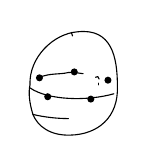
\begin{tikzpicture}[scale=.75,line cap=round,line join=round]
\draw (-.73,-.03) .. controls (-.75,.43) and (-.34,.84) .. (.08,.87)
 .. controls (.65,.93) and (.75,.45) .. (.75,-.05)
 .. controls (.77,-.58) and (.42,-.87) .. (-.05,-.88)
 .. controls (-.39,-.89) and (-.60,-.73) .. (-.68,-.53)
 .. controls (-.74,-.34) and (-.76,-.16) .. (-.73,-.03);
\draw (-.73,-.08) .. controls (-.43,-.29) and (.23,-.31) .. (.69,-.18);
\draw (-.60,.09) .. controls (-.36,.18) and (-.25,.14) .. (-.08,.18)
 .. controls (.01,.19) and (.09,.17) .. (.17,.16);
\draw (.38,.10)--(.42,.11)--(.44,.07);
\draw (.43,0)--(.43,-.03);
\draw (.59,.07)--(.61,.02);
\foreach \x/\y in {-.57/.09,.02/.19,.59/.05,-.43/-.23,.30/-.27}
 {\fill (\x,\y) circle(1.7pt);}
\draw (-.68,-.53) .. controls (-.47,-.58) and (-.25,-.60) .. (-.08,-.60);
\draw (-.03,.86)--(-.01,.80);
\end{tikzpicture}}

\textcircled{2} \(\nu=4\) alors \deleted{\(K=\operatorname{Card}I^g=1\)} \inserted{\(K^g=\{P\}\)}, et \(I\setminus\{P\}\) est une orbite. OPS que c’est \(\mu_4\), sur lequel \(\mu_4\) opère, et \(P\) est un pôle : \(\unsure{\infty|0}\). Le groupe total des autom est \(\mathbb Z/4\mathbb Z\simeq\mu_4(k)\).

La catégorie de ces configurations est équivalente à celle des carrés orientés.

\margin{``pyramide carrée''}
\figure{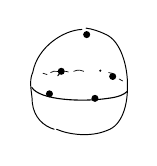
\begin{tikzpicture}[x=.0075cm,y=-.00818cm,line cap=round,line join=round]
\draw[line width=.35pt] (102,14)
 .. controls (71,15) and (27,41) .. (19,80)
 .. controls (11,96) and (18,112) .. (18,128)
 .. controls (21,151) and (37,164) .. (55,169);
\draw[line width=.35pt] (59,169)
 .. controls (79,177) and (115,182) .. (144,171)
 .. controls (171,163) and (179,130) .. (179,104)
 .. controls (180,70) and (167,32) .. (143,22)
 .. controls (132,17) and (119,13) .. (109,12);
\draw[line width=.4pt] (17,104)
 .. controls (31,124) and (102,127) .. (146,121)
 .. controls (163,119) and (172,116) .. (179,110);
\draw[line width=.25pt] (36,82) -- (43,84);
\draw[line width=.25pt] (49,81)
 .. controls (56,76) and (62,82) .. (69,78);
\draw[line width=.25pt] (74,79) -- (79,80);
\draw[line width=.25pt] (88,79)
 .. controls (96,76) and (101,77) .. (105,79);
\draw[line width=.25pt] (147,81) -- (153,82);
\draw[line width=.25pt] (165,91) -- (171,94);
\draw[line width=.35pt] (67,79)--(61,86);
\fill (133,78) circle[radius=.425pt];
\fill (110,22) circle[radius=1.275pt];
\fill (67,79) circle[radius=1.275pt];
\fill (154,87) circle[radius=1.275pt];
\fill (47,114) circle[radius=1.275pt];
\fill (124,121) circle[radius=1.275pt];
\end{tikzpicture}}

\textcircled{3} \(\nu=3\), Alors \deleted{\(\unsure{\Sigma|K}_{\unsure{2}}\)} \(\operatorname{Card}K^g=2\), \inserted{donc \(K^g=\Sigma^g\),} et \(I\setminus K^g\) \inserted{\(=J\)} est une orbite,
\deleted{Le groupe \unsure{total est|des auto}}
\inserted{qu’on peut supposer \(\mu_3\).} La catégorie de ces configurations est équivalente : celle des triangles combinatoires i.e. celle \(\mathrm{Ens}(3)\) des ens \(J\) de Card \(3\).

A \(J\) on associe \(\Sigma_J\unsure{\deleted{\Sigma}|\deleted{g}\Omega|\deleted{G}\Omega}\) avec \(J\cup P_J\) (\(P_J\subset\Sigma_J^{\unsure{g}}\) ens des deux pôles de \(\Sigma_J\) pour corr. \(1\)-\(1\) avec l’ens \(\omega(\unsure{I|J})\) des or. de \(J\), si \(\unsure{k|K}=\mathbb C\)). Groupe des autom. est \(\mathbb D_3\).

\margin{\unsure{Partition|Une partition} \(2\) et \(3\) (par ordre de richesse en symétries)}
\margin{``bitétraèdre''}
\figure{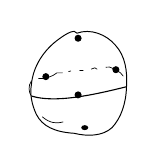
\begin{tikzpicture}[x=.00706cm,y=-.0080cm,line cap=round,line join=round]
\draw[line width=.35pt] (104,16)
 .. controls (128,8) and (157,18) .. (173,35)
 .. controls (191,52) and (195,77) .. (193,102)
 .. controls (192,128) and (183,151) .. (167,166)
 .. controls (150,180) and (122,180) .. (99,175)
 .. controls (64,173) and (42,164) .. (31,145)
 .. controls (23,130) and (19,113) .. (22,98)
 .. controls (25,68) and (45,42) .. (72,25)
 .. controls (86,16) and (100,9) .. (104,16);
\draw[line width=.4pt] (23,116)
 .. controls (64,127) and (130,115) .. (193,101);
\draw[line width=.25pt] (35,88)
 .. controls (46,89) and (60,85) .. (68,79)
 -- (78,79);
\draw[line width=.25pt] (89,77) -- (93,76);
\draw[line width=.25pt] (109,75) -- (115,75);
\draw[line width=.25pt] (130,73) -- (136,71) -- (140,73);
\draw[line width=.25pt] (156,70)
 .. controls (166,68) and (170,74) .. (174,75)
 .. controls (181,77) and (185,81) .. (187,84);
\draw[line width=.25pt] (42,149)
 .. controls (55,159) and (68,160) .. (79,157);
\draw[line width=.25pt] (22,92)..controls(16,99)and(17,110)..(22,116);
\fill (106,24) circle[radius=1.275pt];
\fill (48,85) circle[radius=1.275pt];
\fill (174,74) circle[radius=1.275pt];
\fill (106,114) circle[radius=1.275pt];
\fill (118,166) ellipse[x radius=1.275pt,y radius=.9pt];
\end{tikzpicture}}
\margin{33}

\scanpage{35}
\mspage{2}
\textcircled{4} \(\nu=2\). \deleted{Il y a \unsure{deux cas}} \inserted{\unsure{Dans ce cas|Dans les}} \(K^g=\{P\}\), et \(K\setminus K^g\) \inserted{\(=I\)} est réunion de deux orbites. Ainsi, \(g\) est un autom. \deleted{\unsure{de}} ``universel'' de \(\Sigma\setminus I\) (\(g\in V(\unsure{D_I|\mathbb D_I})\)) et \(P\) est \inserted{\unsure{un de|un|un aut.}} \unsure{\deleted{un}|un} p\textsuperscript{t} fixe. \deleted{\unsure{De|Ce}} Cette fois, la situation \unsure{a} des ``modules'', p.ex. en choisissant une des deux orbites,

\deleted{\unsure{OPS} \unsure{que|pour} l’opération de \(\unsure{g|\langle g\rangle}\) sur elle est celle de \(\mu_2\) \inserted{\(=\{\pm1\}\)} sur \(\mu_2\) \inserted{\(=\unsure{\{\pm1\}|(\pm1)}\)}, et \(P=0\), l’autre orbite est \deleted{\unsure{donnée par}} \unsure{un|une} \(\{t,-t\}\), avec \(\lambda=t^2\ne1,\lambda\in k^\times\) ---
donc \deleted{\(\lambda=\)} \(J=(0,\pm1,\pm\unsure{\sqrt\lambda|t})\) \deleted{\(\unsure{\sqrt\lambda,\sqrt\lambda)|\sqrt\lambda,-\sqrt\lambda)}\)}, avec \(\lambda\in\Sigma(k)\setminus\{0,1,\infty\}\),
\unsure{Si on|en} \deleted{\unsure{change}} change le choix de l’orbite, on trouve
\[
(0,\pm1,\pm\sqrt{1/\lambda}).
\]
Prenons le paramètre \(\rho=\lambda+\frac1\lambda\), \inserted{\(\ne2\)}, donc \(\lambda^2-\rho\lambda+1=0\);
\deleted{\(\lambda=\frac12(\rho\pm\sqrt{\rho^2-4})\)},
on trouve \((0,\pm1,\pm\sqrt{\frac12(\rho\pm\sqrt{\rho^2\unsure{-4}})})\).
\unsure{Eliminer|Comme} \(0,\infty\), et \unsure{deux|les} \unsure{discriminant} \(\lambda\longrightarrow1\), ou --- \unsure{comme} \deleted{\(\unsure{f^\circ|\rho}\)} \(\lambda\), et
\(g(z)=\frac{\lambda}{z}\), p\textsuperscript{ts} fixes}

Cas moins intéressant que les précédents, \unsure{du|de} notre point de vue, car il y a des modules. Quand la structure \((\Sigma,I)\) est une structure carrée, on retrouve soit le cas \(2^\circ\) (si \(g\) laisse stables les deux diagonales), soit le cas \inserted{des sommets} d’un \deleted{\unsure{carré|cas|cube}} carré sphérique équilatéral, et du milieu de l’une des arêtes. \inserted{Est-ce le cas \(1^\circ\) ?} Quand c’est une structure tétraédrale, \(P\) est un des \inserted{\(6\)} sommets de l’octaèdre associé.

\figure{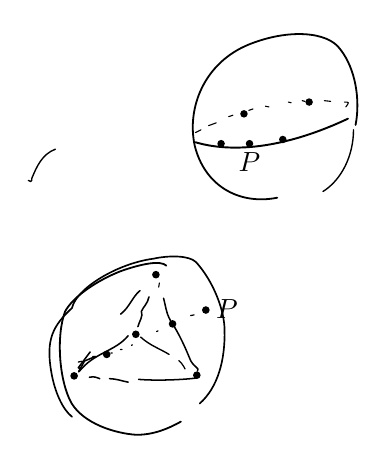
\begin{tikzpicture}[x=.0088cm,y=-.0088cm,line cap=round,line join=round]
% Upper sphere: the contour is open at lower right and has a short right-side gap.
\draw[line width=.65pt] (383,249)
 .. controls (327,260) and (278,231) .. (264,174)
 .. controls (252,119) and (278,54) .. (342,28)
 .. controls (399,5) and (456,9) .. (474,35)
 .. controls (496,63) and (503,108) .. (496,144);
\draw[line width=.5pt] (493,151)
 .. controls (493,188) and (476,223) .. (449,240);
\draw[line width=.7pt] (265,169)
 .. controls (323,186) and (400,175) .. (485,135);
% Rear equatorial arc, with the irregular short dashes visible on the sheet.
\draw[line width=.4pt] (265,155)--(273,151)
 (284,145)--(295,141) (313,132)--(319,130)
 (342,123)--(348,121) (366,117)--(371,118)
 (399,111)--(403,112) (419,109)--(423,110)
 (451,109)--(460,110) (480,111)..controls(487,111)..(482,118);
\foreach \x/\y in {302/171,343/171,391/165,335/128,429/111}
 {\fill (\x,\y) circle[radius=5.4];}
\node[below,inner sep=1pt] at (343,179) {$P$};
% Detached curved stroke at the left, without a supplied arrowhead.
\draw[line width=.5pt] (63,179)..controls(44,186)and(36,204)..(29,221)
 ..controls(30,227)and(25,226)..(24,224);
\begin{scope}[shift={(25,305)}]
% Lower sphere: the two left-hand contours and the open lower-right contour.
\draw[line width=.65pt] (198,42)
 ..controls(190,34)and(163,39)..(132,50)
 ..controls(99,63)and(64,86)..(52,108)
 ..controls(39,143)and(43,207)..(61,240)
 ..controls(79,270)and(124,284)..(155,286)
 ..controls(180,286)and(201,277)..(219,267);
\draw[line width=.6pt] (62,103)
 ..controls(34,129)and(24,149)..(32,195)
 ..controls(37,225)and(49,250)..(62,260);
\draw[line width=.6pt] (62,103)
 ..controls(68,75)and(127,39)..(179,32)
 ..controls(202,27)and(231,27)..(241,37)
 ..controls(267,66)and(282,108)..(282,135)
 ..controls(283,179)and(272,218)..(246,241);
% Broken outer triangular sides and rear branches, preserving their gaps.
\draw[line width=.55pt] (160,78)..controls(149,87)and(145,102)..(132,112);
\draw[line width=.55pt] (88.1778,166.4)--(71.1111,189.1556)--(74.6667,191.6444);
\draw[line width=.55pt] (71.4667,194.8444)--(80,179.5556)--(95.2889,173.1556);
\draw[line width=.55pt] (194,89)..controls(198,104)and(198,113)..(207,126)
 ..controls(216,140)and(224,157)..(231,174)
 ..controls(236,189)and(247,189)..(243,194);
\draw[line width=.55pt] (87,203)..controls(94,201)and(99,204)..(102,205)
 (116,205)..controls(126,205)and(136,209)..(143,210)
 (158,206)..controls(180,208)and(219,207)..(242,204);
\draw[line width=.55pt] (173,87)..controls(171,97)and(165,101)..(162,108)
 ..controls(165,115)and(159,122)..(157,130);
\draw[line width=.55pt] (143,143)..controls(124,166)and(94,167)..(72,195);
\draw[line width=.5pt] (161,145)..controls(174,157)and(189,162)..(202,170);
\draw[line width=.45pt] (216,179)..controls(220,182)and(223,187)..(225,191);
% Dotted oblique slant, including the short dash next to P.
\draw[line width=.45pt] (71,181)--(76,180) (92,173)--(97,173)
 (118,168)--(120,168) (132,163)--(134,163)
 (148,157)--(149,156) (184,137)--(186,136)
 (233,114)--(238,113);
\draw[line width=.4pt] (188,67)--(187,73);
\foreach \x/\y in {183/55,65/201,242/200,154/141,112/170,207/126,255/106}
 {\fill (\x,\y) circle[radius=5.5];}
\node[right,inner sep=2pt] at (261,105) {$P$};
\end{scope}
\end{tikzpicture}}

\uline{Cas des antiautomorphismes \inserted{\(\sigma\)} de} \(\Sigma\) laissant \uline{stables} \(K\). \inserted{\unsure{(}Cas \(k=\mathbb C\))} Comme \unsure{il|\(\sigma\)} est d’ordre pair, on voit qu’il \deleted{\unsure{et|a}} \unsure{a|.} un p\textsuperscript{t} fixe au moins dans \(K\), donc dans \(\Sigma\), et étant d’ordre fini, on sait qu’il est d’ordre \(2\), il correspond à une structure réelle sur \(\Sigma\), \deleted{\unsure{et}}
On distingue suivant le cardinal de \(K^\sigma\), qui est \(1,3\), ou \(\unsure{6|5}\).
\margin{34}

\scanpage{36}
\mspage{3}

a) \(K^\sigma=K\) --- on trouve ess.\textsuperscript{t} les points réels de
\(M_{0,\unsure{5|\bar I}}^{!}\simeq\mathrm{Sym}_2^*(U_{0,3})\),
\deleted{\unsure{Le cas|un cas}} de dim réelle \(2\) : contient le cas \(1^\circ\) (pentagonal)

b) \(\operatorname{Card}K^\sigma=3\), En prenant un repère \(0,1,\infty\) dans \(K^\sigma\), on trouve que
\[
K=\{0,1,\infty,\lambda,\bar\lambda\},\quad
\lambda\in\text{demi-plan de Poincaré},\quad\text{dim réelle }2.
\]
Contient le cas \(3^\circ\) (bitétraédral)
\margin{OPS \(\sigma z=\bar z\) \deleted{\unsure{pour} \(\sigma z=\bar z\)}}

c) \(\operatorname{Card}K^\sigma=1\), i.e. \deleted{\unsure{?}} \(K^\sigma=\{P\}\),
\inserted{\unsure{Soit} \(K\setminus K^\sigma=I\), donc}
\deleted{On \unsure{prend comme repère|prend pour coordonnées|peut prendre comme points} \(\unsure{t_0|\infty}\), et on choisit un p\textsuperscript{t} \(0\) tel que \(0=\sigma0\). \unsure{OP|\(\sigma P\)}}

\((\Sigma,I)\) est un syst. de \(4\) pts sur une sphère complexe,
\deleted{muni d’} \inserted{\unsure{admettant}} un \unsure{antiautomorphisme|anti-isomorphisme}
\deleted{\(\unsure{\sigma}\)} involutif (``conjugaison''), ils sont bien connus et de dim
modulaire \uline{réelle} \(1\), de plus le choix d’un p\textsuperscript{t}
réel supplémentaire \(P\) fait une dim. de
plus, soit dim réelle totale \(2\) encore.
(Contient le cas pyramidal carré, \(2^\circ\))

\figure{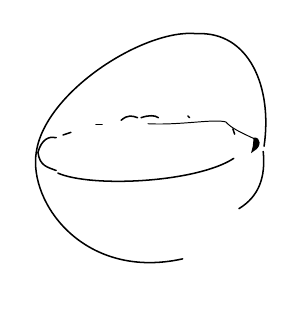
\begin{tikzpicture}[x=.011cm,y=-.011cm,line width=.55pt,line cap=round,line join=round]
\draw (289,1180) .. controls (176,1205) and (111,1116) .. (120,1057)
 .. controls (130,987) and (245,914) .. (305,920)
 .. controls (366,917) and (393,982) .. (383,1050);
\draw (382,1056) .. controls (385,1086) and (377,1108) .. (354,1122);
\draw (122,1057) .. controls (126,1042) and (135,1038) .. (143,1040);
\draw (151,1037)--(160,1034);
\draw (189,1025)--(196,1025);
\draw (218,1020) .. controls (226,1013) and (231,1015) .. (237,1017);
\draw (241,1017) .. controls (250,1014) and (257,1014) .. (261,1017);
\draw (295,1015)--(297,1017);
\draw[line width=.35pt] (249,1024) .. controls (286,1026) and (326,1018) .. (339,1022)
 .. controls (345,1029) and (356,1034) .. (371,1041);
\draw (347,1030)--(349,1036);
\draw (122,1057) .. controls (124,1073) and (133,1074) .. (143,1078);
\draw (145,1081) .. controls (184,1098) and (305,1092) .. (348,1064);
\fill (371,1040) .. controls (380,1039) and (380,1051) .. (372,1055)
 --(368,1058)--(370,1050)--cycle;
\end{tikzpicture}}

\figure{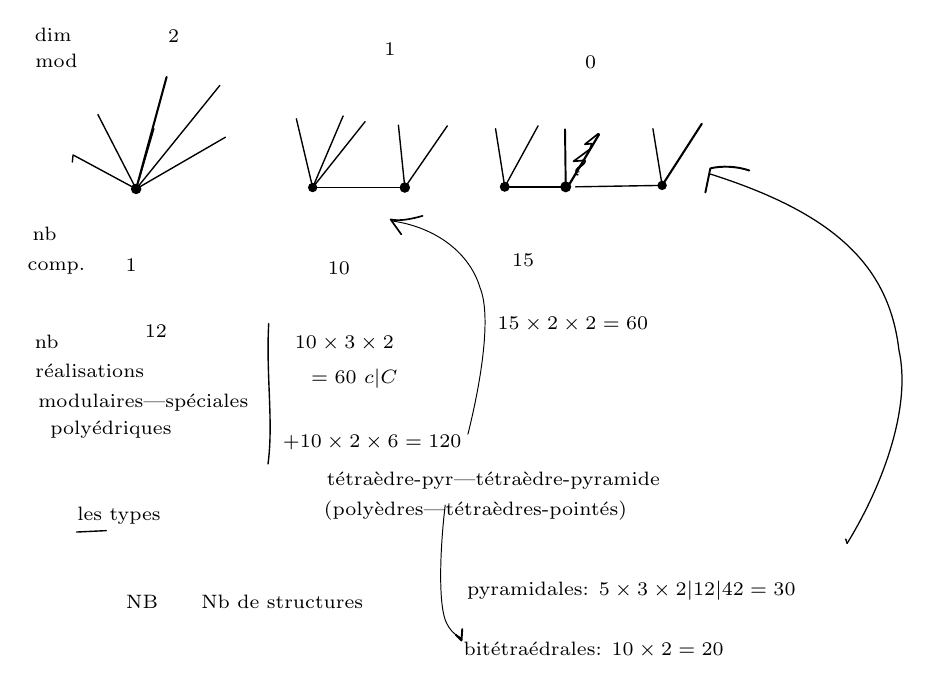
\begin{tikzpicture}[x=.009cm,y=-.009cm,line width=.5pt,line cap=round,line join=round,font=\scriptsize,inner sep=0pt]
\node[anchor=west] at (30,1535) {dim};
\node[anchor=west] at (31,1572) {mod};
\node at (227,1538) {$2$};
\node at (532,1556) {$1$};
\node at (815,1575) {$0$};
% Five free branches at a single vertex.
\draw (174,1753)--(85,1705)--(84,1715);
\draw (174,1753)--(120,1648);
\draw[line width=.75pt] (174,1753)--(217,1595);
\draw (178,1740)--(199,1668);
\draw (174,1753)--(292,1607);
\draw (174,1753)--(300,1680);
\fill (174,1753) circle (1.9pt);
% Two joined vertices and their three plus two branches.
\draw (423,1751)--(553,1751);
\draw (423,1751)--(400,1654);
\draw (423,1751)--(466,1650);
\draw (423,1751)--(497,1658);
\draw (553,1751)--(544,1663);
\draw (553,1751)--(613,1664);
\fill (423,1751) circle (1.7pt);
\fill (553,1751) circle (1.9pt);
% The sloping extra middle branch is crossed out; the upright remains.
\draw (694,1750)--(780,1750);
\draw (794,1750)--(916,1748);
\draw (694,1750)--(681,1668);
\draw (694,1750)--(741,1664);
\draw[line width=.7pt] (780,1750)--(779,1669);
\draw[line width=.8pt] (783,1750)--(827,1676);
\begin{scope}[shift={(760,1645)}]
\draw[line width=.6pt] (37,88) .. controls (32,89) and (33,81) .. (44,74)
 .. controls (50,69) and (47,65) .. (43,68)
 -- (31,69) -- (54,52) -- (57,44) -- (47,45) -- (66,30);
\draw[line width=.35pt] (39,84) .. controls (31,85) and (33,79) .. (43,74);
\end{scope}
\draw (916,1748)--(903,1668);
\draw[line width=.75pt] (916,1748)--(972,1661);
\fill (694,1750) circle (1.8pt);
\fill (780,1750) circle (2pt);
\fill (916,1748) circle (1.7pt);
\node[anchor=west] at (27,1816) {nb};
\node[anchor=west] at (20,1865) {comp.};
\node at (167,1860) {$1$};
\node at (460,1865) {$10$};
\node at (720,1854) {$15$};
\node at (202,1954) {$12$};
\node[anchor=west] at (30,1968) {nb};
\node[anchor=west] at (31,2010) {réalisations};
\node[anchor=west] at (35,2054) {\unsure{modulaires|spéciales}};
\node[anchor=west] at (52,2092) {\deleted{\unsure{polyédriques}}};
\draw (361,1943) .. controls (357,2015) and (368,2082) .. (360,2141);
\node[anchor=west] at (397,1971) {$10\times3\times2$};
\node[anchor=west] at (420,2020) {$=60\ \unsure{c|C}$};
\node[anchor=west] at (380,2110) {$+10\times2\times6=120$};
\node[anchor=west] at (683,1944) {$15\times2\times2=60$};
\node[anchor=west] at (442,2164) {\deleted{\unsure{tétraèdre-pyr|tétraèdre-pyramide}}};
\node[anchor=west] at (438,2207) {\inserted{(\unsure{polyèdres|tétraèdres}-pointés)}};
\node[anchor=west] at (90,2214) {\deleted{\unsure{les types}}};
\draw (90,2237)--(132,2235);
\node[anchor=west] at (159,2335) {\uline{NB}};
\node[anchor=west] at (265,2335) {Nb de structures};
\node[anchor=west] at (640,2320) {pyramidales: $5\times3\times\unsure{2|\deleted{1}\inserted{2}|\deleted{4}\inserted{2}}=30$};
\node[anchor=west] at (635,2404) {bitétraédrales: $10\times2=20$};
% Open upper heads, a hooked right tail, and a separate lower arrow.
\begin{scope}[shift={(525,1695)}]
\draw[line width=.35pt] (117,404) .. controls (137,324) and (150,235) .. (134,197)
 .. controls (120,150) and (74,112) .. (9,103);
\draw[line width=.6pt] (23,122) -- (8,101) .. controls (21,104) and (39,100) .. (53,96);
\draw[line width=.45pt] (652,558) .. controls (703,475) and (743,365) .. (725,285)
 .. controls (711,165) and (632,92) .. (459,37);
\draw[line width=.7pt] (452,63) -- (459,29)
 .. controls (475,25) and (497,26) .. (514,32);
\draw[line width=.5pt] (652,558) -- (650,552);
\draw[line width=.35pt] (85,504) .. controls (78,562) and (75,637) .. (85,666)
 .. controls (91,681) and (99,687) .. (107,691);
\draw[line width=.68pt] (100,687) -- (108,695) -- (109,679);
\end{scope}
\end{tikzpicture}}

\figure{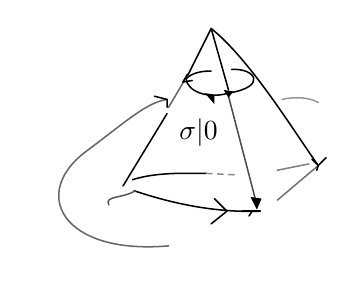
\begin{tikzpicture}[x=.02cm,y=-.02cm,line width=.55pt,line cap=round,line join=round]
\draw (1235,2700)--(1220,2730);
\draw[black!60] (1218,2733)--(1208,2750);
\draw (1207,2754)--(1179,2800);
\draw (1235,2700) .. controls (1260,2720) and (1288,2766) .. (1303,2787);
\draw (1235,2700)--(1246,2739);
\draw[black!70] (1246,2743)--(1264,2812);
\fill (1260,2807)--(1264,2815)--(1267,2808)--cycle;
\draw (1185,2796) .. controls (1201,2791) and (1219,2792) .. (1232,2792);
\draw[black!45,dash pattern=on 2pt off 2pt] (1232,2792)--(1252,2793);
\draw[black!50] (1277,2790)--(1297,2786);
\draw[black!55] (1277,2809)--(1303,2787);
\draw (1303,2787)--(1308,2782);
\draw (1299,2783)--(1303,2787)--(1302,2790);
\draw (1186,2803) .. controls (1210,2811) and (1237,2817) .. (1266,2816);
\draw (1237,2808)--(1245,2816)--(1235,2824);
\draw[line width=.9pt] (1255,2816)--(1266,2816);
\draw (1261,2816)--(1259,2819);
\draw[black!65] (1170,2812) .. controls (1167,2806) and (1179,2808) .. (1187,2803);
% Outer loop, with the visible head at its upper end.
\draw[black!60] (1208,2838) .. controls (1140,2844) and (1119,2804) .. (1157,2777)
 .. controls (1181,2759) and (1194,2747) .. (1207,2745);
\draw (1199,2743)--(1207,2745)--(1207,2750);
\draw[black!40] (1280,2745) .. controls (1289,2743) and (1298,2744) .. (1303,2747);
% Small upper circuit, its breaks and dark directional contacts.
\draw (1219,2732) .. controls (1223,2728) and (1229,2727) .. (1235,2727);
\draw (1248,2726) .. controls (1263,2725) and (1271,2737) .. (1246,2741)
 .. controls (1233,2745) and (1220,2740) .. (1219,2732);
\draw (1220,2729)--(1217,2734)--(1223,2733);
\fill (1231,2741)--(1237,2748)--(1237,2742)--cycle;
\fill (1243,2739)--(1246,2744)--(1249,2740)--cycle;
\node at (1227,2766) {$\unsure{\sigma|0}$};
\end{tikzpicture}}

\margin{35}

\scanpage{37}
\margin{36}
le carré est
\[
 \lambda=\frac{(\xi+\eta)^2}{\xi\wedge\eta}
 =\deleted{\unsure{\frac{\xi}{\eta}}}\frac{\xi}{\eta}+\frac{\eta}{\xi}+2
\]
et dont la connaissance nous permet de retrouver la situation de départ à iso.
\uline{\unsure{un|aux}} \uline{unique} près. La condition à mettre sur
$\lambda$ est que $\lambda-4\ne0$ i.e.
\[
 \lambda'\overset{\unsure{\mathrm{df}}}{=}\lambda-
 2= \frac{\xi}{\eta}+\frac{\eta}{\xi}\ne2
\]
En termes d'une base \deleted{\unsure{de}} $e_1$ de $L_1$,
satisfaisant $e_1^4=e=\xi\wedge\eta$, donnant une base $e_1^2$ de $L_2$,
la situation est déterminée par \inserted{la paire d'éléments distincts}
$\xi_0,\eta_0\in\mathbb C$ $(\xi=\xi_0e_1^2,\ \eta=\eta_0e_1^2)$,
satisfaisant $\xi_0\eta_0=1$, ou encore par
$\mu=\xi_0+\eta_0\inserted{\in\mathbb C}$, satisfaisant $\mu^2-4\ne0$,
$\xi_0$ et $\eta_0$ se récupérant comme solutions de l'équation
\[
 z^2-\mu z+1=0,
\]
l'équation \tikz[baseline=(ineq.base)]{
\node[inner sep=1pt] (ineq) {$\mu^2-4\ne0\quad\text{i.e.}\quad\unsure{\mu^2|\mu}\ne\pm2$};
\draw ([xshift=-2pt,yshift=4pt]ineq.south west)
 .. controls ([xshift=-2pt,yshift=-2pt]ineq.south west) and
 ([xshift=-1pt,yshift=-3pt]ineq.south west) .. ([xshift=2pt,yshift=-3pt]ineq.south west)
 -- ([xshift=-2pt,yshift=-3pt]ineq.south east)
 .. controls ([xshift=1pt,yshift=-3pt]ineq.south east) and
 ([xshift=2pt,yshift=-1pt]ineq.south east) .. ([xshift=2pt,yshift=1pt]ineq.south east);
\draw ([xshift=5pt,yshift=2pt]ineq.south east) -- ([xshift=5pt,yshift=2pt]ineq.north east);
}
s'exprime par les \inserted{2} solutions sont distinctes (néc\textsuperscript{t} non nulles car leur
produit est $1$). \deleted{\unsure{Les}} On récupère $I$ comme l'ens des solutions de
\[
 z^4-\mu z^2+1=0
\]
\[
 I=\left\{\pm\sqrt{\tfrac12\left(\mu\pm\sqrt{\mu^2-4}\right.}\right\}
 =\left\{\pm\sqrt{\mu'\pm\sqrt{\mu'^2-1}}\right\}
\]
\margin{\begin{tikzpicture}[baseline=(eq.base)]
\node[inner sep=1pt] (eq) {où $\mu'=\tfrac12\mu$};
\node[anchor=west,inner sep=1pt] (ie) at (eq.east) {i.e.};
\draw ([xshift=-2pt]eq.west)
 .. controls ([xshift=2pt,yshift=3pt]eq.north west) and
 ([xshift=-4pt,yshift=4pt]eq.north east) .. ([xshift=0pt,yshift=2pt]eq.north east)
 .. controls ([xshift=2pt]eq.north east) and
 ([xshift=-2pt,yshift=-2pt]ie.south west) .. ([xshift=2pt,yshift=-2pt]ie.south west)
 -- ([yshift=-2pt]ie.south east);
\end{tikzpicture}}

\scanpage{38}
\uline{Autom d'ordre deux d'une sphère holomorphe} \inserted{$\Sigma$}
\uline{\unsure{à|:}} \inserted{un $K$ de} $5$ \uline{pts marqués} : Un pt fixe exactement dans $K$,
soit $K=\{P\}\amalg I$, et $\Sigma$ est munie de $I$ et d'un autom
\inserted{$\sigma$} d'ordre $2$, stabilisant $I$,
\inserted{$I$ ne contenant pas de pt fixe de $\sigma$.}
Donc cel. revient à la donnée

a) D'une sphère hol. $\Sigma$, un autom \inserted{$\sigma$} d'ordre $2$
et un pt fixe marqué --- appelant celui-ci $\infty$, et l'autre pt fixe $0$,
cela revient à la donnée d'un torseur $T_1\ (= \Sigma\setminus\{0,\infty\})$
sous $\mathbb C^*$, i.e. d'une droite vectorielle complexe $L_1$
$(T_1=L_1^*)$

b) D'une paire d'orbites \inserted{(distinctes)} de
$\{\pm1\}\subset\mathbb C^*$ opérant sur $T_1=L_1^*$.
Introduisant $T_2=T^{\wedge2}$\inserted{$\simeq L_2^*$, où
$L_2=L_1^{\otimes2}$,}, cel revient à la donnée d'une paire de pts
\inserted{$\{\xi,\eta\}$} (distincts) de $T_2$.
Considérons alors le pt
\[
 e=\xi\wedge\eta=\eta\wedge\xi
 \in T_4=T^{\wedge4}\simeq L_4^*
 \quad(\text{où }L_4=L_1^{\otimes4})
\]
on a donc un
\[
 \mathrm{iso}\quad T^{\wedge4}\simeq\mathbf1_{\mathbb C^*}
\]
d'où une réduction du groupe structural \inserted{de $T$}
de $\mathbb C^*$ : $\mu_4(\mathbb C_*)\simeq\mathbb Z/4\mathbb Z$.
On peut dire que la donnée de $\{\xi,\eta\}$ revient à celle de
$e=\xi\wedge\eta\inserted{\in T_4}$ et de
$\xi+\eta\in\unsure{t_2|T_2}$, soumis à la condition que
$(\xi\unsure{\wedge|+}\eta)^2-4\xi\wedge\eta\ne0$ \deleted{\unsure{un}}.
Notons \deleted{$\unsure{\xi^2+\eta^2-2\xi\wedge\eta\ne}$}
que $T_2$ admet une réduction du groupe structural $\mathbb C^*$ :
$\{\pm1\}$, par la bibase $\pm\sqrt e$, donc $\xi+\eta$
définit un \unsure{élt} de $\mathbb C$ à un signe près, dont
\deleted{$\unsure{(\xi+\eta)^2}$}
\margin{37}

\scanpage{39}

Changer la base \unsure{\deleted{\illegible{1}}|---} \(e_1\) en \(\zeta e_1\) (où \(\zeta^4=1\))
\deleted{revient à} change\deleted{\unsure{r}} \deleted{\unsure{par}}
\(\{\xi,\eta\}\) en \(\{\zeta^2\xi,\zeta^2\eta\}\),
donc \(\mu\) en \(\zeta^2\mu\), qui est donc
égal à \(\mu\) si \(\zeta\in\{\pm1\}\), égal à \(-\mu\) si
\(\zeta\in\{\pm i\}\).

La multiplicité modulaire pour les
structures envisagées, \uline{rigidifiées} par la
donnée de \(e_1\), est donc \(\mathbb P^1\setminus\{0,\pm2,\infty\}\)
Elle s'envoie dans la multiplicité
\(M_{0,5}\) --- il y a lieu de regarder l'effet
sur les groupoïdes fondamentaux.

\margin{38}

\scanpage{41}
\texttt{/*JOB=CRAY2;ACCT=*********,ALL=M06}\qquad\texttt{J0231CNU}

\texttt{// JOB MSGLEVEL=(0,0),MSGCLASS=Z}

\texttt{// EXEC \unsure{CSS3ATCH|CSSBATCH}}

\texttt{//CRAYIN DD *}

\figure{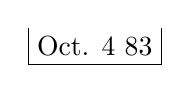
\begin{tikzpicture}[x=1cm,y=1cm]
\node[anchor=base west,inner sep=0pt] (date) at (0,0) {Oct. 4 83};
\draw ([xshift=-3pt,yshift=3pt]date.north west)--([xshift=-3pt,yshift=-3pt]date.south west)--([xshift=3pt,yshift=-3pt]date.south east)--([xshift=3pt,yshift=3pt]date.north east);
\end{tikzpicture}}

\diagram{\begin{tikzcd}[ampersand replacement=\&,column sep=large,row sep=large]
R=RR/\sigma_1\arrow[d]\&
\overset{\sigma_0,\sigma_1}{RR}\arrow[l]\arrow[d,"\mathrm{supp}"]\\
A=\vec A/\sigma\&
\underset{\sigma}{\vec A}\arrow[l]\&
\vec A_0\arrow[l,hook]\arrow[d,"\sigma"]\\
\&\&S\arrow[r,"g"]\&\mathbb N
\end{tikzcd}}

a) $\unsure{\vec\sigma|\bar\sigma}^{2}=\mathrm{id}$, $\sigma$ ss p\textsuperscript{t} fixe

b) supp Compatible avec $\mathbb D_\infty\longrightarrow\{\pm1\}$

c) $RR/D_\infty\underset{\substack{\unsure{\mathrm{bij}}\\[-.4ex]\unsure{\exists}}}{\lhook\joinrel\longrightarrow}
 A=\vec A/\{\pm1\}$

d) (\unsure{évt.}) condition anabélienne (\unsure{ou hyperbolique|cs hyperboliques}) :
$\forall s\in S$, on a
$\deleted{\unsure{2g(s)}}\unsure{:}\ 2g(s)+\nu_s\ge3$
\margin{\[
3\unsure{g_p|g_s}-3+\nu_s\ge0
\]
\[
2\unsure{g_p|g_s}-2+\nu_s\ge\unsure{1}
\]
\[
2g_s+\nu_s\ge3
\]}

1) Somme \unsure{$+$}

\figure{\begin{tikzpicture}[x=1cm,y=.65cm]
\node[anchor=base east,inner sep=0pt] at (.25,0) {4)};
\node[anchor=base west,inner sep=0pt] at (.85,0) {amalgamation (\uline{sans} gommage)};
\node[anchor=base east,inner sep=0pt] at (.25,-1) {5)};
\node[anchor=base west,inner sep=0pt] at (.85,-1) {découpage (en gardant données de recollement)};
\draw (.68,.35) .. controls (.43,.35) and (.52,-.15) .. (.43,-.30)
 .. controls (.32,-.40) and (.32,-.45) .. (.43,-.52)
 .. controls (.52,-.65) and (.43,-1.12) .. (.68,-1.15);
\node[anchor=base east,inner sep=0pt] at (.25,-2.2) {2)};
\node[anchor=base west,inner sep=0pt] at (.85,-2.2) {gommage de \deleted{\unsure{repères}} sommets de marquage.};
\node[anchor=base east,inner sep=0pt] at (.25,-3.2) {3)};
\node[anchor=base west,inner sep=0pt] at (.85,-3.2) {surmarquage};
\draw (.68,-1.85) .. controls (.43,-1.85) and (.52,-2.35) .. (.43,-2.50)
 .. controls (.32,-2.60) and (.32,-2.65) .. (.43,-2.72)
 .. controls (.52,-2.85) and (.43,-3.32) .. (.68,-3.35);
\draw (-.15,-3.86)--(6.2,-3.69);
\draw (-.15,-3.99)--(6.2,-3.82);
\node[anchor=base east,inner sep=0pt] at (.25,-4.8) {6)};
\node[anchor=base west,inner sep=0pt] at (.85,-4.8) {Bouchage des trous (gommage des cercles de raccord)};
\node[anchor=base east,inner sep=0pt] at (.25,-5.9) {7)};
\node[anchor=base west,inner sep=0pt] at (.85,-5.9) {gommage de cercles de découpage};
\draw (-.55,-6.19)--(1.04,-6.09);
\draw (-.55,-6.31)--(1.04,-6.22);
\end{tikzpicture}}

\margin{\unsure{4,5} inverses l'un de l'autre (à condition que l'on ne découpe que par
des cercles \uline{marqués})}

\margin{\uline{Cercles de découpage}

\uline{Cercles de raccord}

Sommets de marquage \inserted{ou de rigidification}
$\left\{\begin{array}{l}\text{périphériques}\\\text{intérieurs}\end{array}\right.$

Cercles marqués (non marqués)}
\margin{\begin{tabular}{|l}
\uline{graphes} \uline{pondérés}\\[.7ex]
graphes \unsure{bipondérés|bipondéré} \deleted{\uuline{\unsure{marqués|marqué}}}\\[.7ex]
graphes pondérés marqués
\end{tabular}}

Le \deleted{\unsure{point|foncteur}} \uline{twist}
\inserted{\unsure{\uline{relatif}|\deleted{relatif}}}
$\tau_r$ \deleted{$(r\in\mathbb Q)$} à un cercle de
découpage marqué, est défini en termes de 4) 5), avec
$\tau_r=\mathrm{id}$ si $r\in\mathbb Z$.
\diagram{\begin{tikzpicture}
\node[inner sep=8pt] (boxed) {\begin{tikzcd}[ampersand replacement=\&]
S_1\mathcal T_{g,\nu}^{\pm1}\arrow[r]\&
\mathcal T_{g,\nu}^{\pm1}\arrow[r]\&
\mathrm{Ens}(\unsure{\nu|\omega})\times[\pm1]
\end{tikzcd}};
\draw ([yshift=-9pt]boxed.north west)--(boxed.south west)--(boxed.south east)--([yshift=-9pt]boxed.north east);
\draw (boxed.north west)--(boxed.north east)--([yshift=-4pt]boxed.north east);
\end{tikzpicture}}
\deleted{$\unsure{\mathcal T_{g,\nu}^{\pm}\ \mathcal T_{\mathrm{top}}\
(TSR)_{g,\nu}|\mathcal T_{g,\nu}^{\pm}\ \mathcal T_{\mathrm{top}}\
(TSD)_{g,\nu}}$} :
$T_{g,\nu}S_\alpha$

Mais l'\uline{iso} de \uline{twist} \deleted{\unsure{est un}} relatif à
un cercle (de découpage ou de raccord, marqué ou pas):
\inserted{\unsure{ou de recollement}}
$\tau_r$ (pour un cercle de découpage marqué) est
\begin{tikzpicture}[baseline=(une.base)]
\node[anchor=base west,inner sep=0pt] (une) at (0,0) {une nouvelle};
\draw ([xshift=2pt,yshift=-1pt]une.south west)--([yshift=-1pt]une.south east);
\end{tikzpicture}
\uline{structure} \unsure{importante}

\margin{type combinatoire d'un objet de
$\deleted{\unsure{\mathcal T}}\unsure{,}\ SD\mathcal T_{\mathrm{top}}$

Catégorie des types combinatoires}

\figure{\begin{tikzpicture}[x=1cm,y=1cm]
\node at (0,0) {$\deleted{\mathcal T S}$};
\node at (2,0) {$\deleted{\mathcal T D}$};
\node at (1,-.9) {$\deleted{\mathcal T SD}$};
\node at (1,-2.2) {$\deleted{\unsure{\mathcal T^*(\Gamma)}}$};
\draw (3.3,.15)--(3.3,-1.95);
\node[anchor=west,inner sep=0pt] at (3.5,-.9) {\unsure{avec $\omega^L$|avec inv}\qquad$\pm$};
\node[anchor=west,inner sep=0pt] at (3.5,-2.05) {$\mathcal T$};
\node[anchor=north west,inner sep=0pt] at (3.5,-2.5) {$\begin{array}{c|c}
S\mathcal T&ST\\
SD\mathcal T&SDT\\
D\mathcal T&DT
\end{array}$};
\end{tikzpicture}}

\diagram{\begin{tikzcd}[ampersand replacement=\&,column sep=small,row sep=small]
\&\&\mathcal T\arrow[dl,dash]\arrow[dr,dash]\&\begin{array}{l}\text{graphes pond.}\\\text{discrets}\end{array}\&\\
\text{graphes b}\&S\mathcal T\arrow[dr,dash]\&\&D\mathcal T\arrow[dl,dash]\&\text{graphes pondérés}\\
\&\&SD\mathcal T\&\text{graphes}\&
\end{tikzcd}}

\diagram{\begin{tikzcd}[ampersand replacement=\&,column sep=small,row sep=small]
\&\unsure{t|\mathbb L}\arrow[dl,dash,bend right=5]\arrow[dr,dash,bend right=10]\&\\
s\unsure{t|\mathbb L}\arrow[dr,dash,bend left=10]\&\&d\unsure{t|\mathbb L}\arrow[dl,dash,bend right=8]\\
\&sd\unsure{t|\mathbb L}\&
\end{tikzcd}}
\margin{40}

\scanpage{42}
opérations de recollage / sommes

\figure{\begin{tikzpicture}[x=1cm,y=1cm,every node/.style={anchor=west,inner sep=0pt,outer sep=0pt}]
\node at (1.65,0) {objets; diagrammes};
\node at (0.75,-0.62) {cercles de raccord (ou de recollage)};
\node at (0.75,-1.02) {cercles de découpage};
\node at (0.78,-1.47) {Sommets de \uline{marquage}};
\node[align=left] at (5.65,-1.47) {(périphériques\\intérieurs};
\node at (0.51,-2.08) {cercles marqués et non marqués};
\draw (0.24,0.31) .. controls (0.03,0.32) and (0.12,-0.53) .. (0.03,-0.84)
  .. controls (0.00,-0.95) and (-0.04,-0.96) .. (-0.10,-0.96)
  .. controls (0.13,-0.93) and (0.12,-1.12) .. (0.10,-1.31)
  .. controls (0.08,-1.87) and (0.07,-2.20) .. (0.29,-2.24);
\draw (0.55,-0.45) .. controls (0.48,-0.50) and (0.56,-0.69) .. (0.54,-0.78)
  .. controls (0.53,-0.82) and (0.49,-0.83) .. (0.46,-0.81)
  .. controls (0.56,-0.83) and (0.50,-1.02) .. (0.57,-1.15);
\end{tikzpicture}}

\begin{tabular}{@{}l@{}}
[condition \deleted{\unsure{de}} ``anabélienne''\\
\hspace{1.4em}ou de ``stabilité'']
\end{tabular}

\diagram{\begin{tikzcd}[ampersand replacement=\&,column sep=small,row sep=small]
\&\makebox[0pt][r]{\(\deleted{\unsure{SD}}\)\,}\mathcal T\arrow[dl,dash]\arrow[dr,dash]\arrow[rrrr]\&\&\&\&\unsure{t|\mathbb L}\arrow[dl,dash]\arrow[dr,dash]\&\\
S\mathcal T\arrow[dr,dash]\arrow[rr,dash]\&\&D\mathcal T\arrow[dl,dash]\arrow[rr,bend left=15]\arrow[rrrr,bend right=20]\&\&s\unsure{t|\mathbb L}\arrow[dr,dash]\&\&d\unsure{t|\mathbb L}\arrow[dl,dash]\\
\&SD\mathcal T\arrow[rrrr]\&\&\&\&sd\unsure{t|\mathbb L}\&\\
\&\&\&\&\&\text{\makebox[0pt]{types combinatoires}}\&
\end{tikzcd}}

Catalogue opérations $+$ structures

\figure{\begin{tikzpicture}[x=1cm,y=1cm,every node/.style={anchor=west,inner sep=0pt,outer sep=0pt}]
\node at (0,0) {1)};
\node at (0.90,0) {Somme};
\node at (0,-0.85) {2)};
\node at (0.90,-0.85) {gommage (partiel) \unsure{de|du} marquage};
\node at (0,-1.65) {3)};
\node at (0.90,-1.65) {surmarquage};
\draw (0.48,0.22) .. controls (0.38,-0.05) and (0.44,-0.55) .. (0.46,-1.10)
  .. controls (0.52,-1.72) and (0.50,-1.95) .. (0.28,-1.97);
\draw[<->] (9.10,-0.72) -- (9.10,-1.24);
\node at (0,-2.55) {4)};
\node at (0.90,-2.55) {découpage (partiel)\unsure{,}};
\node at (0,-3.40) {5)};
\node at (0.90,-3.40) {amalgamation ou recollage};
\draw (0.70,-3.63) -- (2.62,-3.60);
\node at (6.95,-3.40) {\deleted{\unsure{avec (données de}}};
\node at (7.06,-2.96) {\inserted{sans gommage!}};
\node at (10.66,-3.24) {)};
\draw[<->] (12.00,-2.49) -- (12.00,-3.18);
\node at (0,-4.50) {6)};
\node at (0.90,-4.50) {bouchage de trous (= gommage de cercles de raccord)};
\draw (0.29,-2.02) .. controls (0.48,-2.03) and (0.47,-2.20) .. (0.46,-2.59)
  -- (0.47,-4.61) .. controls (0.48,-4.79) and (0.57,-4.83) .. (0.68,-4.95);
\node at (0,-5.30) {7)};
\node at (0.90,-5.30) {gommage de cercles intérieurs};
\end{tikzpicture}}

foncteurs et iso ``twist''
\margin{41}

\scanpage{43}
\unsure{les|Les} douze avatars principaux de la
\unsure{Tours|Tour} de Teichmüller :
\deleted{\unsure{systèmes|système} de groupoïdes}

groupoïde $\mathrm{RTD}\ldots$ avec structures
\inserted{(``les 10 opérations''), \unsure{réalis.}}
diverses dans un groupoïde
dont le \deleted{\unsure{représentant}} le plus élémentaire est
$\deleted{\unsure{\mathrm{RTD}}},\ \mathbb T_{\mathrm{top}}$

\diagram{\begin{tikzcd}[ampersand replacement=\&,row sep=1.5em,column sep=1em]
\&\mathbb T_{\mathrm{top}}\&
\begin{gathered}
\text{cas topologique (à bord \deleted{\unsure{géod.}} toriques}
\end{gathered}\&
\begin{gathered}\text{découpage}\\\text{top.}\end{gathered}\\
\mathbb T'_{\mathrm{diff}}\arrow[r,shift left]\arrow[from=r,shift left]\&
\mathbb T_{\mathrm{diff}}\arrow[u]\&
\begin{gathered}
\text{cas différentiable (à \deleted{pts \unsure{trous} pointés)}}\\
\text{\inserted{bord toriques)}}\\
\text{\deleted{(avec \unsure{peu de|presque} pts marqués)}}
\end{gathered}\&\text{déc. diff}\\
\begin{gathered}\uparrow\\\text{à pts marqués}\\
\text{et \unsure{drs.|dirs.} tangts}\\\text{complexes}\\\text{\unsure{qconq.|qcq.}}\end{gathered}\&
\mathbb T_{\mathrm{an}}\arrow[u]\&
\begin{gathered}
\text{cas }\inserted{\mathbb C\text{-}}\text{analytique (à bord \unsure{\deleted{g}|g}toriques)}
\end{gathered}\&
\begin{gathered}\text{déc. en}\\\unsure{\mathbb C^\infty?}\end{gathered}\\
\mathbb T'_{\mathrm{an}}\arrow[ur,shift left]\arrow[from=ur,shift left]\&\&\&\\
\&\mathbb T_{\mathrm{hyp}}\arrow[uu]\&
\begin{gathered}\text{cas hyperbolique (à bord géodésique)}\end{gathered}\&
\text{déc. hyp.}\\
\mathbb T'_{\mathrm{hyp}}\arrow[uu]\arrow[ur,shift left]\arrow[from=ur,shift left]\&\&\&\\
\&\mathbb T_{\mathbb C\mathrm{alg}}\arrow[uu]\&
\begin{gathered}
\text{cas }\mathbb C\text{-algébrique (courbes MD,}\\
\text{munies d'une \deleted{rigidification} de}\\
\text{propagation \unsure{de cercles|des cercles|du cercle} aux pts}\\
\text{doubles, plus pts marqués}
\end{gathered}\&\\
\&\mathbb T_{\overline{\mathbb Q}\text{-}\mathrm{alg}}\arrow[u]\&
\begin{gathered}
\text{cas }\overline{\mathbb Q}\text{-alg. (\unsure{propagation}}\\
\text{\unsure{descente|descendant}}\ 
\unsure{\mathrm{Gal}|\deleted{\mathrm G}\mathrm{al}}/\overline{\mathbb Q}\text{)}
\end{gathered}\&\\
\&\mathbb T_{\mathrm{comb}}\arrow[u]\&
\begin{gathered}
\text{cas combinatoire, via cartes orientées}\\
\text{\uline{à bord} \unsure{quadr.|qcq.}, avec sommets marqués}
\end{gathered}\&\\
\&\mathbb T_{\mathrm{L\acute ego}}\arrow[u]\&
\begin{gathered}\text{cas combinatoire ``Légo'', avec}\\
\text{les 10 pièces du jeu}\end{gathered}\&\\
\&\mathbb T_{\mathbb P}\arrow[u]\&
\begin{gathered}\text{cas combinatoire ``pantalonique'',}\\
\text{avec comme seules pièces les}\\
\text{\deleted{``\unsure{pantalon|pantalons}''} \unsure{triades|triade}.}\end{gathered}\&
\end{tikzcd}}
\margin{42}

\scanpage{44}
\mspage{1}
\uline{Groupoïdes de Teichmüller}.

\textcircled{1} Cas topologique.

La variante la plus simple est
\[
\mathcal T^+_{\mathrm{top}}\quad\text{ou}\quad\mathcal T_{\mathrm{top}}
\]
(\uline{groupoïde de Teichmüller} \uuline{orienté} \uline{topologique})

\uline{objets} : surfaces \uline{à bord} compactes orientées $(\Sigma)$\unsure{,|.}

\uline{flèches} : classes d'isotopie d'iso (conservant l'orientation)

\margin{Finalement, tant qu'on ne travaille pas au point de vue
arithmétique, il semble que c'est le gros $\mathcal T^\pm$ qui sera
le plus utilisé; \deleted{\unsure{tout|d'où}} c'est lui qui
mérite donc ici la notation la plus simple $\mathcal T$,
et le \unsure{gr.\ or.} orienté de s'appeler $\mathcal T^+$.}

Variante immédiate
\[
\mathcal T_{\mathrm{top}}^\pm
\]
(\uline{groupoïde de Teichmüller} \uuline{biorienté} \uline{topologique}) :
mêmes objets, flèches sont les classes d'isotopie d'homéomorphismes
(ne conservant pas néc\textsuperscript{t}. l'orientation).

Soit $[\pm1]$ le groupoïde ayant un seul objet $e$ (par exemple $e=\varnothing$)
et comme groupe d'autom $\pm1$. On a un morphisme de signature
\diagram{\begin{tikzcd}[ampersand replacement=\&]
\mathcal T^\pm_{\mathrm{top}}\arrow[r,"\chi"]\&{[\pm1]}
\end{tikzcd}}
dont la \uline{fibre} \deleted{\unsure{est}} (ou noyau) est
$\mathcal T_{\mathrm{top}}^+=\mathcal T_{\mathrm{top}}$.
\margin{\figure{\begin{tikzpicture}[x=0.27cm,y=0.30cm,every node/.style={anchor=west,inner sep=0pt,outer sep=0pt,font=\tiny}]
\node at (1.2,0) {\unsure{Canulé|Cautèle},};
\node at (0,-1.05) {si on ne se borne};
\node at (-0.1,-2.12) {à des surfaces};
\node at (-0.1,-3.18) {connexes};
\node at (7.8,-2.72) {!};
\draw (7.18,-1.46) -- (7.12,-3.02)
  .. controls (7.13,-3.47) and (6.28,-3.30) .. (5.64,-3.08);
\end{tikzpicture}}}

La variante la plus complexe est
\[
S_*\mathcal TD_{\mathrm{top}}^+\quad\text{ou}\quad
S_*\mathcal TD_{\mathrm{top}},
\]
``\uline{groupoïde de Teichmüller} \inserted{\uline{orienté}}
\uline{spécial dévissé topologique}''
\margin{43}

\scanpage{46}
\mspage{2}
\uline{objets} : Triples $(X,\widetilde\Sigma,
\deleted{\unsure{S}}\inserted{R})$, \unsure{où|ou}

$X$ surface à bord compacte orientée

$\widetilde\Sigma$ sous-variété compacte de $X$
\deleted{\unsure{close}}, $\widetilde\Sigma\supset\partial X$

\begin{tikzpicture}[x=.13cm,y=.13cm,baseline=-.1ex,line width=.5pt]
\draw (.08,.05) .. controls (-.03,.42) and (.24,.67) .. (.62,.89)
 .. controls (.97,.97) and (1.02,.7) .. (.72,.48)
 .. controls (.47,.28) and (.3,.08) .. (.08,.05);
\draw (.12,.15)--(.81,1.08);
\draw (.32,.04)--(.98,.78);
\draw (.11,.62)--(.83,.13);
\end{tikzpicture}
$\deleted{\unsure{S}}R\subset\Sigma\deleted{\unsure{\widetilde\Sigma}}$,
partie finie

\margin{$X,\deleted{\partial X},\Sigma,S$}
\margin{$\widetilde\Sigma=\partial X\amalg\Sigma$

On peut considérer que $R$ rigidifie, \unsure{mais} aussi $\widetilde\Sigma$\ldots{}
que $R$ ``découpe''}

\uline{flèches} : classes d'isotopie d'homéom. conservant l'orientation

\deleted{Variante \unsure{de}}
Les compos. connexes de $\widetilde\Sigma\setminus\partial X
\inserted{=\Sigma}$ sont les \uline{cercles de découpage},
\inserted{celles de $\partial X$ sont les cercles de raccord},
les éléments de $\deleted{\unsure{S}}R$ sont les
\deleted{\unsure{pts de marquage}} \uline{sommets de}
\deleted{\uline{marquage}}\inserted{rigidification},
\deleted{(ou de rigidification)},
\deleted{les \unsure{composantes} connexes de $\partial X$ sont les ``\uline{trous}''}.
Les composantes connexes de $X$ sont les
\deleted{connexes}\inserted{\uline{composants}}
de l'objet envisagé.

Variante $S_*\mathcal TD_{\mathrm{top}}^\pm$, avec
\diagram{\begin{tikzcd}[ampersand replacement=\&,column sep=large]
S_*\mathcal TD_{\mathrm{top}}
\arrow[r,phantom,"{\begin{tikzpicture}[x=1cm,y=1cm,baseline=-.15ex]
\draw (.23,.16) .. controls (-.05,.16) and (-.08,-.02) .. (.15,-.02)--(1.15,.02);
\end{tikzpicture}}" description]\&
S_*\mathcal TD_{\mathrm{top}}^\pm\arrow[r]\&{[\pm1]}
\end{tikzcd}}
comme tantôt.

On a des sous-groupoïdes pleins
\diagram{\(\begin{array}{ccl}
R=\varnothing,\ \Sigma=\unsure{\varnothing}&
\mathcal T_{\mathrm{top}}\quad\text{et}\quad\mathcal T^\pm_{\mathrm{top}}&\\
\deleted{\unsure{R=\widetilde\Sigma=\varnothing}}&&\\
\Sigma=\deleted{\unsure{\partial X}}\unsure{\partial X|\varnothing\deleted{X}}&
S_*\mathcal T_{\mathrm{top}}\quad\text{et}\quad S_*\mathcal T^\pm_{\mathrm{top}}&
\begin{gathered}
\text{(groupoïdes de Teich-}\\
\text{müller \uline{spéciaux}}\\[-.1ex]
\text{\inserted{\begin{tikzpicture}[baseline=(rig.base)]
\node[anchor=base west,inner sep=0pt] (rig) at (0,0) {ou \uline{rigidifiés}};
\draw ([xshift=-2pt,yshift=2pt]rig.west)
 .. controls ([xshift=-6pt,yshift=-3pt]rig.west) and ([xshift=-2pt,yshift=-5pt]rig.south west) .. ([yshift=-5pt]rig.south west)
 --([yshift=-5pt]rig.south east)
 .. controls ([xshift=4pt,yshift=-5pt]rig.south east) and ([xshift=5pt,yshift=-1pt]rig.east) .. ([xshift=5pt,yshift=3pt]rig.east);
\end{tikzpicture}}}\\
\text{(topologiques orientés)}
\end{gathered}\\
R\text{ quelconque}&&\\
R=\varnothing&
\mathcal T_{\deleted{\unsure{\mathrm{top}}}}D_{\mathrm{top}}\quad\text{et}\quad\mathcal TD^\pm_{\mathrm{top}}&
\end{array}\)}
(Cas pas intéressant je crois, sauf pour $\Sigma=\unsure{\varnothing}$
également)

\margin{MD = ``modulaire'' ou \unsure{Mumford}--Deligne}

\deleted{\unsure{Dé}} \uline{Détermination} du
$\pi_0(S_*\mathcal TD_{\mathrm{top}})
 \xrightarrow{\sim}\pi_0(S_*\mathcal TD^\pm_{\mathrm{top}})$.

On introduit les \uline{graphes} \deleted{\unsure{MD}} bipondérés
\margin{45}

\scanpage{47}
\mspage{3)}
qui forment un groupoïde $\deleted{\unsure{\mathrm{MD}}}.\ \mathrm{Grbip}$
ou $(\mathrm{Grabipond})$

Objets : graphes \inserted{finis} $(S,\vec A,\sigma,o)$
\inserted{$+$ structures suppl.}
(pouvant avoir des sommets isolés, des boucles fermées, a fortiori
plusieurs arêtes entre deux sommets, et aussi des ``\uline{arêtes} libres''
\inserted{(``sommets'', ``arcs'')}
correspondant aux pts fixes de $\sigma$)
$S,\inserted{\vec A}$ ens. finis, $\sigma:\vec A\longrightarrow\vec A$ involution,
$o:\vec A\longrightarrow S$ appl. ``origine''.
On se donne de plus
\diagram{\begin{tikzcd}[ampersand replacement=\&]
S\arrow[r,"\deleted{\unsure{g}}\inserted{\gamma}"]\&\mathbb N
\end{tikzcd}}
(application ``genre'' ou ``poids'')

\diagram{\begin{tikzcd}[ampersand replacement=\&]
\deleted{\unsure{\vec A^{\sigma}|\vec A}}=A_\ell
\arrow[r,"r\,\deleted{\unsure{\rho}}\,2"]\&\mathbb N
\end{tikzcd}}
(application \deleted{\unsure{rigi}} \deleted{\unsure{rigidification}}
``indice de rigidification'')

\deleted{``\unsure{arêtes libres}''}
\deleted{$\unsure{A_\ell}\overset{\mathrm{def}}{\subset}\vec A/\sigma$
``ens. des \unsure{sommets supplémentaires}''}

\margin{pas assez précis comme donnée. \unsure{La|la} pondération d'une arête doit être
remplacée par celle d'un pol. comb. $T_a$ avec
$\omega(\unsure{T|T_a})\simeq\omega(a)$}

\margin{\begin{tikzpicture}[x=1cm,y=1cm]
\node[anchor=north west,align=left,inner sep=0pt] at (0,0)
{J'ai indiqué une pondé-\\ration des sommets,\\mais pas des arêtes};
\draw (2.65,.22) .. controls (3.85,.35) and (4.08,.15) .. (4.08,-.38)
.. controls (4.02,-.98) and (1.45,-1.08) .. (.15,-1.22)
.. controls (-.20,-1.26) and (-.34,-1.45) .. (-.36,-1.62);
\end{tikzpicture}}

\figure{\begin{tikzpicture}[x=.013cm,y=-.013cm,line width=.55pt]
\coordinate (a) at (73,199); \coordinate (b) at (227,200);
\coordinate (c) at (361,196); \coordinate (d) at (300,104);
\coordinate (e) at (201,103); \coordinate (f) at (243,282);
\coordinate (g) at (471,177);
\draw (a) .. controls (122,173) and (205,164) .. (b);
\draw (a) .. controls (130,201) and (190,193) .. (b);
\draw (a) .. controls (130,231) and (195,237) .. (b);
\draw (a) .. controls (24,234) and (10,327) .. (30,329)
.. controls (60,326) and (75,259) .. (a);
\draw (a)--(51,65);
\draw (a)--(87,155);
\draw[black!30,line width=.35pt] (89,149)--(103,107) (106,98)--(118,63);
\draw (118,63)--(120,55);
\draw (b) .. controls (270,205) and (318,204) .. (c);
\draw (b)--(d) (d)--(c);
\draw (b) .. controls (237,216) and (241,261) .. (f);
\draw (b) .. controls (237,164) and (215,121) .. (e);
\draw (e)--(d);
\draw (e) .. controls (231,85) and (282,78) .. (d);
\draw (d)--(335,4) (d)--(387,57)
(d) .. controls (334,109) and (365,115) .. (387,115);
\draw (c) .. controls (350,235) and (332,302) .. (330,339);
\draw (c) .. controls (397,171) and (430,179) .. (g);
\foreach \p in {a,b,c,d,e,f,g}{\fill (\p) circle[radius=5];}
\fill[white] (226,201) circle[radius=1.5];
\fill[white] (244,281) circle[radius=1.6];
\node[left] at (65,195) {$0$};
\node[above right] at (239,204) {$2$};
\node[above right] at (360,191) {$0$};
\node[above left] at (297,97) {$4$};
\node[above] at (201,96) {$13$};
\node[right] at (249,280) {$1$};
\node[above right] at (472,175) {$3$};
\fill (130,303) circle[radius=4.5];
\node[below left] at (126,305) {$2$};
\fill (132,424) circle[radius=5];
\node[left] at (122,426) {$0$};
\draw (132,424) .. controls (140,402) and (143,375) .. (138,360);
\draw (132,424)--(168,384);
\draw[black!35,line width=.35pt] (168,384)--(196,350);
\draw (196,350)--(203,342);
\draw (132,424) .. controls (181,401) and (213,428) .. (259,440);
\fill (51,520) ellipse[x radius=7,y radius=5];
\fill[white] (51,520) ellipse[x radius=3.4,y radius=1.2];
\node[left] at (42,518) {$3$};
\draw (51,520) .. controls (105,487) and (187,484) .. (190,527)
.. controls (195,578) and (119,564) .. (51,520);
\end{tikzpicture}}

\deleted{Ou encore, posons $\widetilde S=S\amalg A_\ell$, (identif.
à l'ens de \uline{tous} les ``sommets'',
\inserted{\unsure{apparents|marqués}} \deleted{\unsure{marqués}} et
``\uline{marqués}'' (i.e. $\in S$) et ``\unsure{libres}''
\inserted{(i.e. correspondant à $\unsure{\alpha|a}\in A_\ell$)}
du graphe), l'on donne
\diagram{\begin{tikzcd}[ampersand replacement=\&]
\widetilde S\arrow[r,"\pi"]\&\mathbb N
\end{tikzcd}}}
(\uline{pondération} du graphe)

\margin{\diagram{\begin{tikzpicture}[x=1cm,y=1cm]
\node at (0,0) {$\widetilde S=S\amalg$};
\node at (1.55,0) {$\deleted{\unsure{S_\ell}}$};
\node at (3.05,0) {\deleted{\unsure{apparents}}};
\node at (1.47,-.85) {$\inserted{A_\ell}$};
\draw (1.34,-.37) .. controls (1.12,-.40) and (1.18,-.25) .. (1.25,-.13);
\draw (1.33,-.18)--(1.35,-.48);
\end{tikzpicture}}
\[
\widetilde A=\vec A/\sigma=A\amalg A_\ell
\]
\diagram{\begin{tikzpicture}[x=1cm,y=1cm,>=stealth]
\node (va) at (0,0) {$\vec A$};
\node at (.55,0) {$=$};
\node (a0) at (1.25,0) {$\vec A_0$};
\node at (1.96,0) {$\amalg$};
\node (al) at (2.65,0) {$\vec A_\ell$};
\draw (.88,-.27) .. controls (.91,-.52) and (1.12,-.48) .. (1.25,-.43)
.. controls (1.39,-.55) and (1.55,-.47) .. (1.63,-.43);
\node at (1.25,-.78) {$\vec A\setminus\vec A^\sigma$};
\draw (2.28,-.28)--(2.28,-.44)--(3.02,-.44)--(3.02,-.28);
\node at (2.65,-.78) {$\vec A^\sigma$};
\draw[->] (.18,-.77)--(.18,-2.42);
\draw[thin] (-.02,-.28)--(-.15,-.42)--(-.20,-1.27)--(-.10,-1.22)
--(-.21,-1.76)--(-.34,-2.08);
\draw[thin] (-.10,-.38)--(-.03,-1.15)--(-.14,-1.51)--(.01,-1.95)
--(-.08,-2.04)--(-.16,-1.80)--(-.25,-2.10);
\draw[thin] (-.23,-1.86)--(-.02,-1.83) (-.25,-1.91)--(-.06,-2.00)
(-.15,-1.25)--(-.01,-1.16);
\draw[->] (1.25,-1.04)--(1.25,-2.32);
\node[right] at (1.27,-1.51) {$\mathrm{deg}\,2$};
\draw[->] (2.65,-1.04)--(2.65,-2.32);
\node[right] at (2.67,-1.51) {$\mathrm{deg}\,1$};
\node at (0,-2.75) {$\widetilde A$};
\node at (.55,-2.75) {$=$};
\node at (1.25,-2.75) {$A$};
\node at (1.96,-2.75) {$\amalg$};
\node at (2.65,-2.75) {$A_\ell$};
\end{tikzpicture}}
Ordre d'un sommet
\diagram{\begin{tikzpicture}[x=1cm,y=1cm]
\node[anchor=east] at (0,0) {$\sigma(s)=$};
\node at (.65,0) {$\sigma_\ell(s)$};
\node[anchor=west] at (1.31,0) {$+\sigma_0(s)$};
\draw (.12,-.22)--(.12,-.37)--(1.18,-.37)--(1.18,-.22);
\node[anchor=north,align=left,inner sep=0pt] at (.90,-.50)
{correspond\\aux ``trous''\\ou cercles\\de recollage};
\end{tikzpicture}}}

La donnée du \uline{graphe} sous-jacent à un graphe
$\deleted{\mathrm{MD}}\inserted{\mathrm{bip.}}$ revient à celle d'un graphe
``ordinaire'' correspondant (sans arêtes libres,
i.e. où $\sigma$ opère ss pts fixes), i.e.
\[
\left(S,(\vec A\setminus\vec A^\sigma),
\sigma|(\vec A\setminus\vec A^\sigma),
o|(\vec A\setminus\vec A^\sigma)\right),
\]
\uline{plus} un ensemble \inserted{fini} $A_\ell$
(\uline{arêtes \deleted{\illegible{1}}} libres)
\deleted{ou ``sommets-trous)} et une application
\diagram{\begin{tikzcd}[ampersand replacement=\&]A_\ell\arrow[r]\&S\end{tikzcd}}

\uline{Flèches} Les iso. de telles structures
\margin{46}
